\documentclass[envcountsect,aspectratio=43]{beamer}


\usepackage{pythontex} 
\usepackage{etex}
\usefonttheme[onlymath]{serif}
\usepackage[utf8x]{inputenc}
\usepackage[brazilian]{babel}
\usepackage{amsthm,amssymb}
%\usepackage{graphicx}
\usepackage{wrapfig}

\usepackage{color}

\usepackage{multicol}
\usepackage{makecell}
\usepackage{syntonly}
\hypersetup{colorlinks,linkcolor=,urlcolor=blue}


\usepackage{pgf,tikz}
\usetikzlibrary{calc}
\usetikzlibrary{positioning}
\usetikzlibrary{decorations.pathreplacing}
\usepackage{tkz-euclide,tikz-3dplot}

%---------------- tabu package 
\usepackage{xcolor}
\usepackage{colortbl}
\usepackage{tabu}

%-------------------------------

%\newcommand{\code}[1]{{\colorbox{gray}{\texttt{#1}}}

%\syntaxonly
%\includeonly{determinantes}
%\includeonlyframes{conicas,comp} 



\usepackage[labelformat=empty]{caption}
\setbeamertemplate{caption}[numbered]{}


\usetheme{Madrid}
\usecolortheme{beaver}

\setbeamertemplate{theorems}[numbered]


\setbeamertemplate{enumerate items}[circle]
\newtheorem{nada}{Nada}


\theoremstyle{definition}
\newtheorem{defin}[nada]{Defini\c c\~ao}
\newtheorem{prop}[nada]{Proposi\c c\~ao}

\newtheorem{corol}[nada]{Corol\'ario}

\newtheorem{teo}[nada]{Teorema}

\newtheorem{lema}[nada]{Lema}



\newtheorem{outline}{\timesbold outline rem proof}

\newtheorem{obs}[nada]{Observação}
\newtheorem{afir}{Afirmação}





\makeatletter
\def\th@exercicio{%
	\normalfont % body font
	\def\inserttheoremblockenv{alertblock}  
}
\theoremstyle{exercicio}
\newtheorem*{exer}{
\includegraphics[scale=0.06]{w-brainb.png} Exercício}
\makeatother

\newtheorem{casa}{
\includegraphics[scale=0.035]{w-homework.png} Para Casa}
\makeatother




\makeatletter
\def\th@something{%
	\normalfont % body font
	\def\inserttheoremblockenv{exampleblock}  
}
\theoremstyle{something}
\newtheorem*{exe}{
\includegraphics[scale=0.3]{exemplo.png} Exemplo }
\makeatother

%\setbeamercolor{block title}{bg=cyan, fg=white}

\newtheorem*{casa-comp}{
\includegraphics[scale=0.035]{w-homework-comp.png} Tarefa Computacional}
\makeatother

\makeatletter
\def\th@resp{%
	\normalfont % body font
	\def\inserttheoremblockenv{block}  
}
\theoremstyle{resp}
\newtheorem*{resp}{
\includegraphics[scale=0.01]{White_check.png} Resposta}
\makeatother


\makeatletter
\def\th@desafio{%
	\normalfont % body font
	\def\inserttheoremblockenv{alertblock}  
}

\theoremstyle{desafio}
\newtheorem*{desafio}{\includegraphics[scale=0.02]{desafio-branco.png} Desafio}
\makeatother


%%%%%%%%%%%%%%%%%%%%%%%%%%%%%%%%%%%%%%%%%%%%%%%%%%%%%%%%%%%%%%%%%%%%%%%%%%%%%%%%%%%%%%%

\newcommand{\cqd}{\hfill \framebox[7pt]{} \mbox{} \medskip}
\newcommand{\dem}{\noindent {\bf Demonstra\c c\~ao:}}
\newcommand{\dest}{\textcolor{blue}}
\newcommand{\R}{\mathbb{R}}
\newcommand{\vect}[1]{\overrightarrow{#1}}
\newcommand{\vt}[1]{\overrightarrow{#1}}
\newcommand{\dt}[1]{\textcolor{blue}{#1}}
\newcommand{\ang}{\widehat}
\newcommand{\n}[1]{\|#1\|}
\newcommand{\pe}[2]{\langle #1,#2\rangle}
\newcommand{\sen}{\operatorname{sen}} 
\newcommand{\tg}{\operatorname{tg}}     
\newcommand{\proj}{\operatorname{proj}}
\newcommand{\pv}[2]{#1\times #2}
\newcommand{\pmt}[3]{[{#1},{#2},{#3}]}
\newcommand{\ex}{\textcolor{structure}{\large{Exemplo\ \ }}}
\newcommand{\dps}{\displaystyle}
\newcommand{\senh}{\operatorname{senh}}
\newcommand{\tgh}{\operatorname{tgh}}
\newcommand{\sech}{\operatorname{sech}}
\newcommand{\mc}{\textordmasculine\ }
\newcommand{\fm}{\textordfeminine\ }

\newcommand{\pyl}[1]{\py{sp.latex(#1)}}

%%%%%%%%%%%%%%%%%%%%%%%%%%%%%%%%%%%%%%%%%%%%%%%%%%%%%%%%%%%%%%%%%%%%%%%%%%%%%%%%%%%%%%%


\begin{document}

%\setbeamercovered{transparent}
\title[GAAL]{Geometria Analítica e Álgebra Linear\\
	\normalsize{GAAL}}
\author[Reginaldo Demarque]{
\[
{\footnotesize {\color{blue} \underbrace{\begin{bmatrix}
 a_{11}  & a_{12}  & \cdots &  a_{1n}  \\
 a_{21} & a_{22}  & \cdots  & a_{2n} \\
 \vdots & \vdots & \cdots & \vdots \\
 a_{m1} & a_{m2}  & \cdots  & a_{mn} 
\end{bmatrix}}_{A}}\ \
{\color{red}
\underbrace{\begin{bmatrix}
x_1\\ x_2\\ \vdots \\ x_n
\end{bmatrix}}_{X}
}
=
\underbrace{\begin{bmatrix}
b_1 \\ b_2\\ \vdots \\ b_n
\end{bmatrix}}_{B}.}
\]
%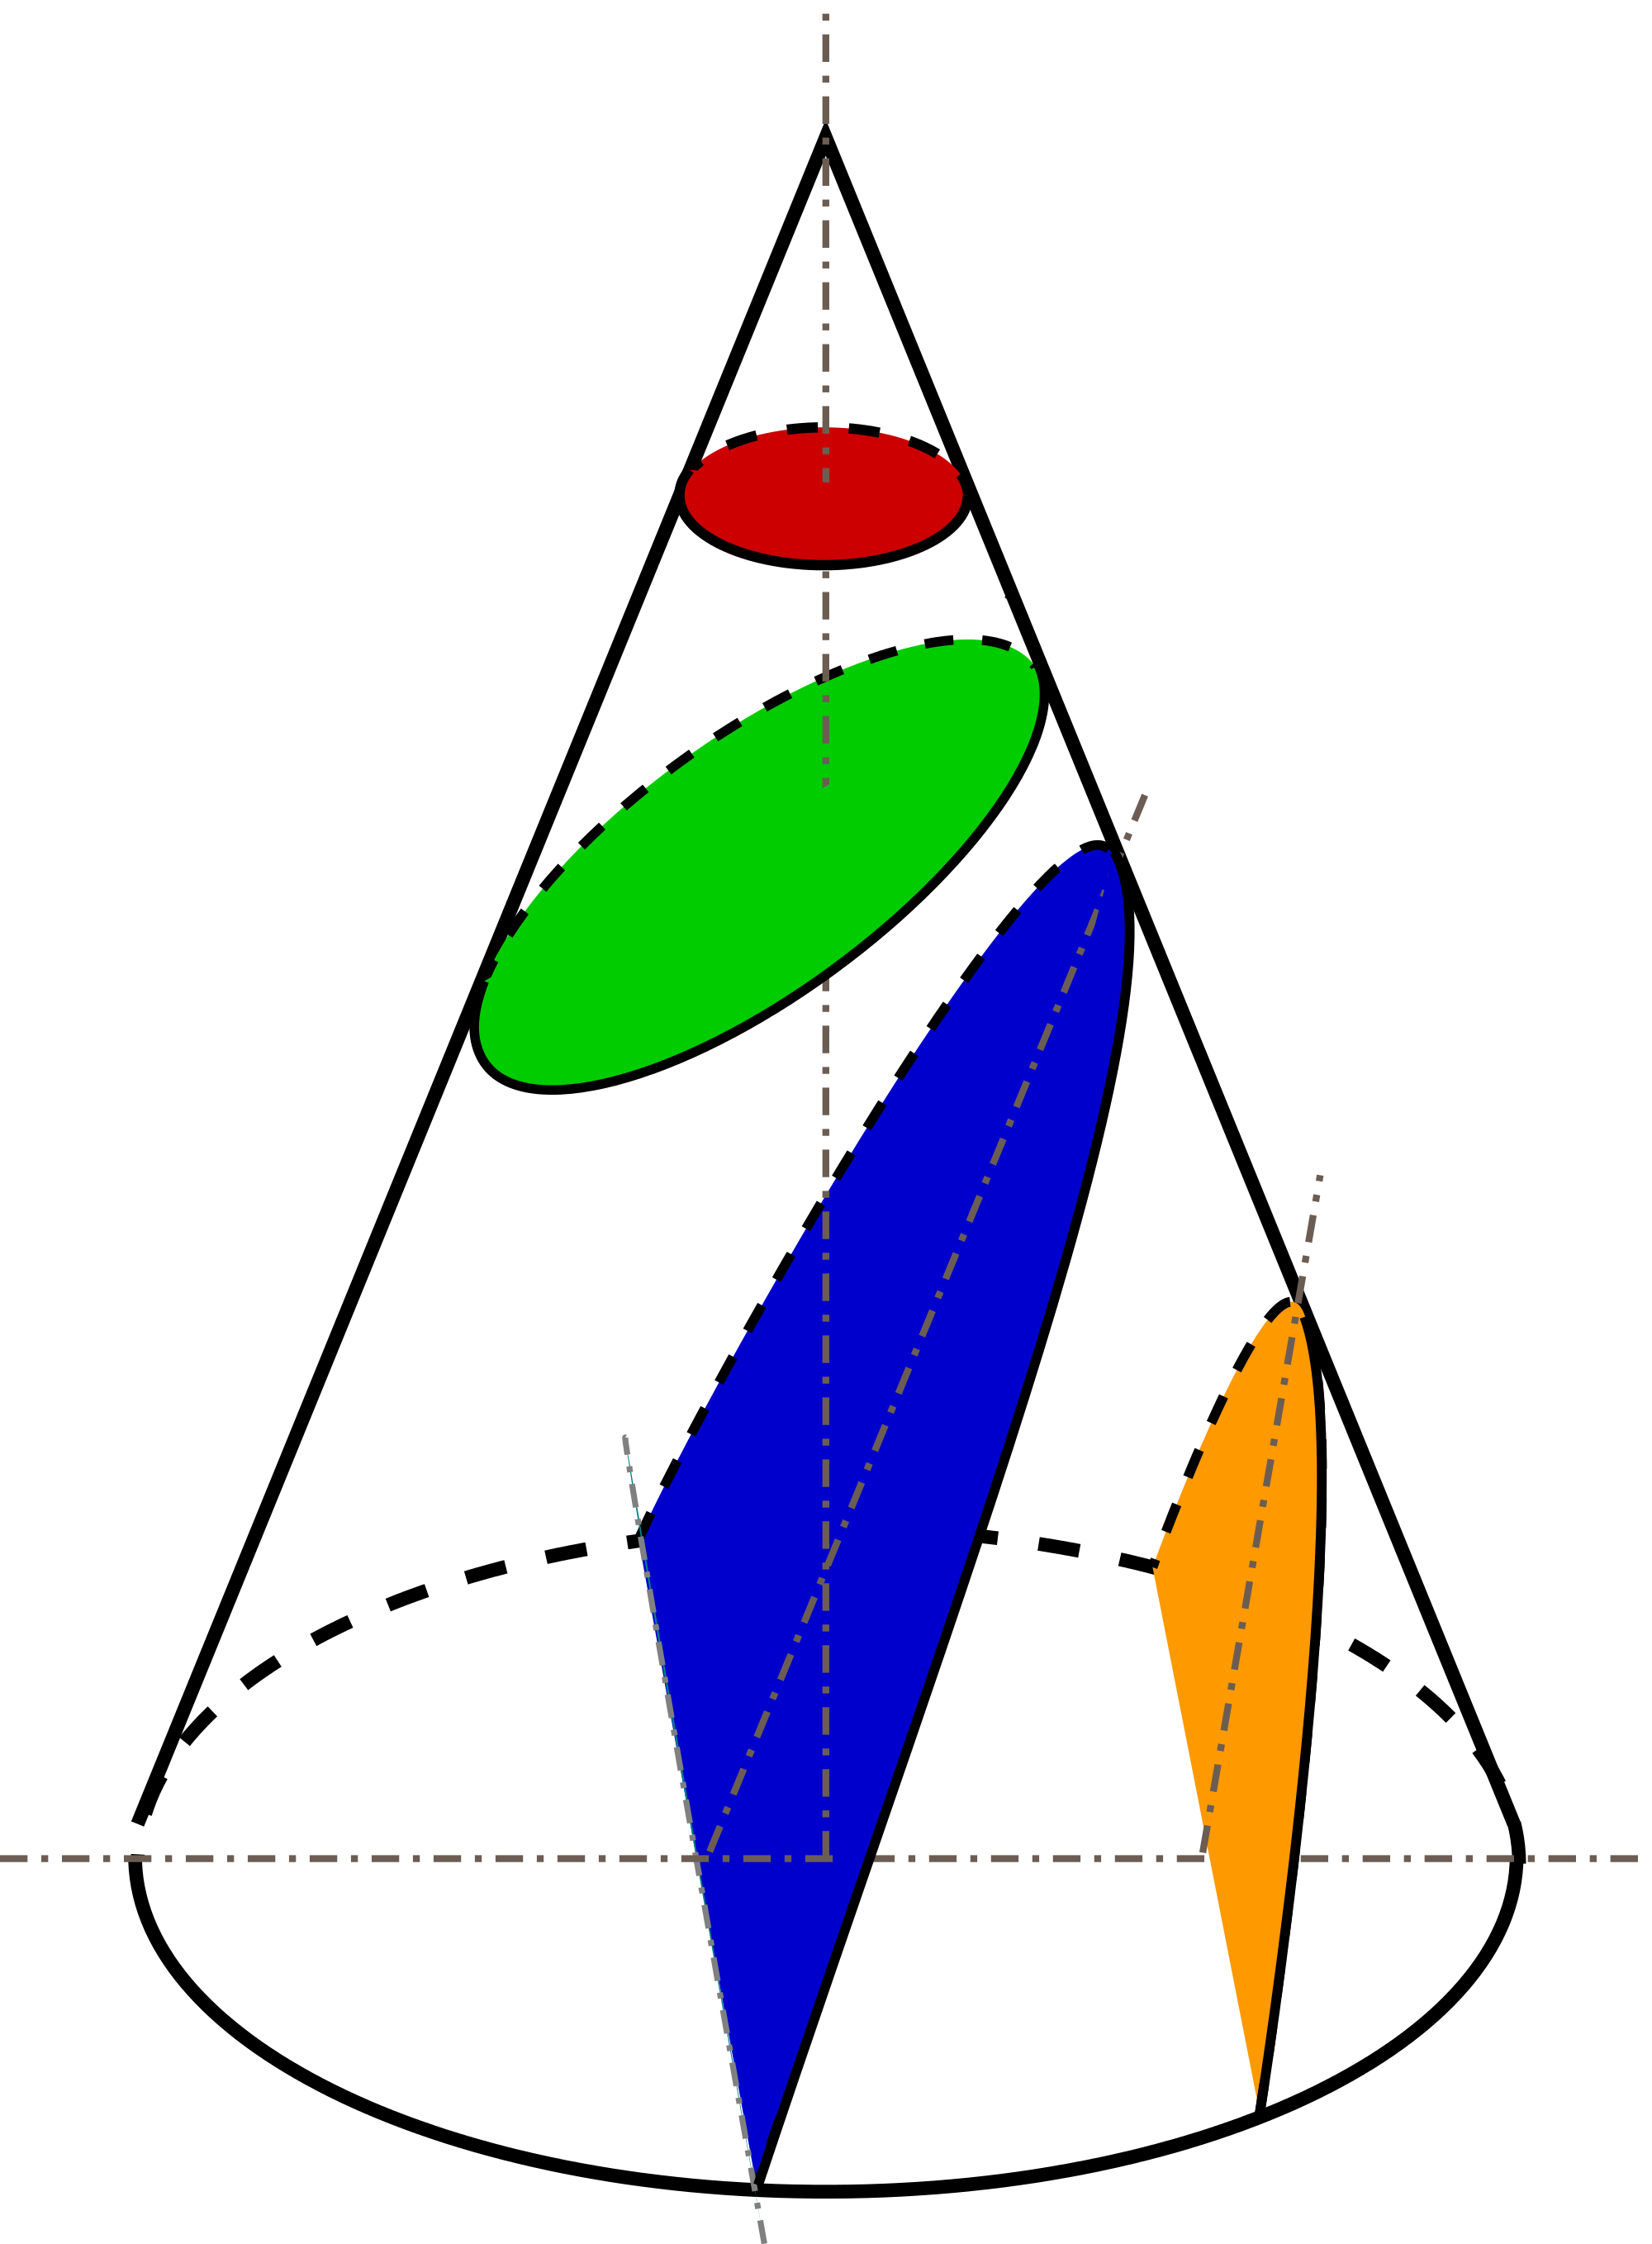
\includegraphics[scale=0.03]{capa.png}\\
	Prof. Reginaldo Demarque}



%%%%%%%%%%%%%%%%%%%%%%%%%%%%%%%%%%%%%%%%%%%%%%%%%%%%%%%%%%%%%%%%%%%%%%%%%%%%

\logo{
\includegraphics[scale=0.03]{UFF_brasao.png}}

\institute[RCN/UFF]{Universidade Federal Fluminense\\
Instituto de Humanidades e Saúde -- RHS\\
Departamento de Ciências da Natureza -- RCN  \\
}
\date{{\color{orange} \today}}


\frame{\titlepage}

%%%%%%%%%%%%%%%%%%%%%%%%%% sumario  %%%%%%%%%%%%%%%%%%%%%%%%%%%%%%%%

\frame{
 \frametitle{Sumário}
 \tableofcontents
}



\AtBeginSection[]
{
 \begin{frame}

  \frametitle{Sumário}
  \tableofcontents[currentsection]

 \end{frame}
}

\section{Vetores}

\subsection*{Plano Cartesiano}
\begin{frame}[label=vetores]{O conjunto $\R^2$}

Denotamos por   $\R^2$ o conjunto formado pelos {\color{blue}pares ordenados} $(x,y)$ tais $x$ $y$ são números reais. O número $x$ chama-se {\color{blue}primeira coordenada ou abcissa} e o número $y$ chama-se {\color{blue}segunda coordenada ou ordenada}. 
\medskip

Podemos representar geometricamente os elementos de $\R^2$ usando um {\color{blue}sistema de coordenadas cartesianas}, que consiste em um plano com um par de eixos perpendiculares $OX$ e $OY$ e que tem a mesma origem.

\begin{exe}
Em um plano, fixado um sistema de coordenadas cartesianas, represente:
\begin{enumerate}
\item Os pontos $P=(1,0)$, $Q=(2,1)$ e $R=(-3,-2)$.
\item Os conjuntos $A=\{(x,y)\in \R^2;\ x=1\}$ e $B=\{(x,y)\in \R^2;\ x=y\}$.
\end{enumerate}
\end{exe}

\end{frame}

\subsection*{Espaços Vetoriais}

\begin{frame}[label=vetores]{Espaços Vetoriais Reais}

Um {\color{blue}espaço vetorial real} $V$ é um conjunto, cujos elementos são chamados {\color{blue} vetores}, no qual estão definidas duas operações:

\begin{itemize}
\item A {\color{blue} adição}, que a cada par de vetores $\vec{u}$,$\vec{v}\in V$ faz corresponder um novo vetor $\vec{u}+\vec{v}$, chamado {\color{blue}vetor soma} de $\vec{u}$ e $\vec{v}$.

\item A {\color{blue} multiplicação por escalar}, que a cada número $\alpha\in \R$ e a cada vetor $\vec{v}\in V$ faz corresponder um vetor $\alpha \vec{v}$, chamado {\color{blue}produto de $\alpha$ por $\vec{v}$}.
\end{itemize}
Além disso, essas operações devem satisfazer, para quaisquer $\vec{u},\vec{v},\vec{w}\in V$ e $\alpha,\beta \in \R$, as seguintes condições:
%\begin{enumerate}
%\item $\vec{u}+\vec{v}=\vec{v}+\vec{u}$ (comutatividade)
%\item $(\vec{u}+\vec{v})+\vec{w}=\vec{u}+(\vec{v}+\vec{w})$ (associatividade)
%\item Existe um vetor $\vec{0}\in V$, chamado {\color{blue}vetor nulo}, tal que
%\[\vec{u}+\vec{0}=\vec{u} \text{ para todo } \vec{u}\in V.\]
%\end{enumerate}
\end{frame}


\begin{frame}[label=vetores]{Espaços Vetoriais Reais}

\begin{enumerate}

\item $\vec{u}+\vec{v}\in V$. (fechamento em relação à adição)
\item $\vec{u}+\vec{v}=\vec{v}+\vec{u}$ (comutatividade)
\item $(\vec{u}+\vec{v})+\vec{w}=\vec{u}+(\vec{v}+\vec{w})$ (associatividade)
\item Existe um vetor $\vec{0}\in V$, chamado {\color{blue}vetor nulo}, tal que
\[\vec{u}+\vec{0}=\vec{u} \text{ para todo } \vec{u}\in V.\]

\item Para cada $\vec{v}\in V$, existe um vetor $\vec{-v}\in E$, chamado {\color{blue}inverso aditivo}, ou {\color{blue}simétrico} de $\vec{v}$, tal que
\[-\vec{v}+\vec{v}=\vec{0}.\]

\item $\alpha \vec{v}\in V$. (fechamento em relação à multiplicação por escalar)

\item $(\alpha+\beta)\vec{v}=\alpha \vec{v}+\beta \vec{v}$ e $\alpha(\vec{u}+\vec{v})=\alpha\vec{v}+\alpha\vec{v}$. (distributividade)

\item $1\cdot \vec{v}=\vec{v}$.
\end{enumerate}
\end{frame}

\subsection*{Vetores no $\R^2$}

\begin{frame}[label=vetores]{O Espaço Vetorial $\R^2$}

O conjunto $\R^2$ torna-se um espaço vetorial quando o munimos com as seguintes  operações: Se $\vec{u}=(u_1,u_2)$,  $\vec{v}=(v_1,v_2)$ e $\alpha\in \R$ então
\[\vec{u}+\vec{v}=(u_1+v_1,u_2+v_2),\]
\[\alpha \vec{v}=(\alpha v_1,\alpha v_2).\]
Neste caso, o {\color{blue}vetor nulo} é $\vec{0}=(0,0)$ e o {\color{blue}simétrico} de $\vec{v}$ é  $-\vec{v}=(-v_1,-v_2)$.


\end{frame}


\begin{frame}[label=vetores]{Representação Geométrica}

Representamos um vetor $\vec{u}=(u_1,u_2)$ de $\R^2$ usando um {\color{blue}segmento orientado} com {\color{blue}ponto inicial} na origem do sistema de coordenadas e {\color{blue}extremidade} no ponto $P=(u_1,u_2)$.

\begin{center}
		\begin{tikzpicture}[scale=1]
		\tikzset{>=latex}
	\draw[help lines, color=gray!30, dashed] (0,0) grid (6,4);
	\draw[->,thick] (0,0)--(6,0) node[right]{$x$};
	\draw[->,thick] (0,0)--(0,4) node[above]{$y$};
%	\foreach \i in {1,...,7}
%	\node[below,scale=0.7] at (\i,0) {$\i$};
%	\foreach \i in {1,...,4}
%	\node[left,scale=0.7] at (0,\i) {$\i$};


\coordinate (O) at (0,0);
\coordinate (E) at (4,2);
\node[left,scale=1] at (0,2) {$u_2$};
\node[below,scale=1] at (4,0) {$u_1$};

	\node[blue] at (O) {\textbullet};
\node[blue,below left] at (O) {$O$};
	
\node[blue] at (E) {\textbullet};
\node[blue,right] at (E) {$P=(u_1,u_2)$};

\node[above] at (2,1) {$\vec{u}$};

\draw[->,ultra thick] (O) -- (E);
	
	\end{tikzpicture}
\end{center}

Neste caso, escrevemos $\vec{u}=\overrightarrow{OP}$. 

\end{frame}

\subsection*{Norma de um vetor}
\begin{frame}[label=vetores]{Norma de um vetor}

O {\color{blue}comprimento} de vetor $\vec{u}$, também chamado de {\color{blue}norma}, é dado por:

\begin{center}
\begin{minipage}{0.5\textwidth}
\begin{block}{}
\[\|\vec{u}\|=\sqrt{u_1^2+u_2^2}.\]
\end{block}
\end{minipage}
\end{center}


\begin{exe}
Represente no plano o vetor $\vec{u}=(1,1)$ e calcule seu comprimento.
\end{exe}
\end{frame}

\subsection*{Lei do Paralelogramo}

\begin{frame}[label=vetores]{Representação Geométrica da Soma}

Dados dois vetores ${\color{red}\vec{u}=(u_1,u_2)}$ e ${\color{blue}\vec{v}=(v_1,v_2)}$ de $\R^2$  o vetor soma 
\[\vec{u}+\vec{v}=(u_1+v_1,u_2+v_2)\]
é obtido pela chamada {\color{blue}lei do paralelogramo}.

\begin{center}
		\begin{tikzpicture}[scale=0.8]
		\tikzset{>=latex}
	\draw[help lines, color=gray!30, dashed] (0,0) grid (6,4);
	\draw[->,thick] (0,0)--(6,0) node[right]{$x$};
	\draw[->,thick] (0,0)--(0,4) node[above]{$y$};



\coordinate (O) at (0,0);
\coordinate (A) at (1,2);
\coordinate (B) at (4,1);
\coordinate (C) at (5,3);
\node[left,scale=.7] at (0,1) {$u_2$};
\node[below,scale=.7] at (4,0) {$u_1$};

\node[left,scale=0.7] at (0,2) {$v_2$};
\node[below,scale=0.7] at (1,0) {$v_1$};

\node[left,scale=.7] at (0,3) {$u_2+v_2$};
\node[below,scale=.7] at (5,0) {$u_1+v_1$};

\node at (2,0.8) {${\color{red}\vec{u}}$};
\node<1> at (0.5,1.5) {${\color{blue}\vec{v}}$};
\node<2> at (4.5,1.5) {${\color{blue}\vec{v}}$};
\node at (2,1.8) {$\vec{u}+\vec{v}$};
\node[blue] at (O) {\textbullet};
\node[blue,below left] at (O) {$O$};
	
\draw<1>[->,ultra thick,blue] (O) -- (A);
\draw[->,ultra thick,red] (O) -- (B);
\draw[->,ultra thick] (O) -- (C);

\draw<1>[dashed,thick] (A) -- (C);
\draw<1>[dashed,thick] (B) -- (C);
\draw<2>[->,ultra thick,blue] (B) -- (C);
	
	\end{tikzpicture}
\end{center}



\end{frame}

\subsection*{Coordenadas de um Vetor}

\begin{frame}[label=vetores]

Dizemos que um segmento de reta orientado {\color{red}$\overrightarrow{AB}$} também representa um vetor ${\color{blue}\vec{u}}$ quando os dois têm mesmo {\color{blue}comprimento, direção e sentido}. Neste caso, escrevemos ${\color{blue}\vec{u}}={\color{red}\overrightarrow{AB}}$.



\begin{center}
		\begin{tikzpicture}[scale=0.8]
		\tikzset{>=latex}
	\draw[help lines, color=gray!30, dashed] (0,0) grid (6,4);
	\draw[->,thick] (0,0)--(6,0) node[right]{$x$};
	\draw[->,thick] (0,0)--(0,4) node[above]{$y$};



\coordinate (O) at (0,0);
\coordinate (A) at (1,2);
\coordinate (B) at (4,1);
\coordinate (C) at (5,3);

\node at (2,0.8) {${\color{blue}\vec{u}}$};
\node[blue,below left] at (O) {$O$};
\node[red,left] at (A) {$A$};
\node[red,right] at (C) {$B$};
	
\draw<1>[->,ultra thick,blue] (O) -- (B);

\draw[->,ultra thick,red] (A) -- (C);
	\end{tikzpicture}
\end{center}

\begin{center}
\begin{minipage}{0.7\textwidth}
\begin{block}{}
Se {\color{red}$A=(a_1,a_2)$} e {\color{red}$B=(b_1,b_2)$} então
\[{\color{red}\overrightarrow{AB}}={\color{blue}\vec{u}=(b_1-a_1,b_2-a_2)}.\]
\end{block}
\end{minipage}
\end{center}

\end{frame}

\begin{frame}[label=vetores]
De uma forma geral temos que 
\begin{center}
\begin{minipage}{0.7\textwidth}
\begin{block}{}
\[\|{\color{red}\overrightarrow{AB}}\|=\sqrt{{\color{blue}(b_1-a_1)^2+(b_2-a_2)^2}}.\]
\end{block}
\end{minipage}
\end{center}


\begin{exe}
Dados $A=(1,1)$, $B=(2,2)$, $C=(-1,0)$ e $D=(0,1)$. Mostre que $\overrightarrow{AB}=\overrightarrow{CD}$ e calcule sua norma.
\end{exe}

\end{frame}




\begin{frame}[label=vetores]


Basta usar a lei do paralelogramo. 

\begin{center}
		\begin{tikzpicture}[scale=0.8]
		\tikzset{>=latex}
	\draw[help lines, color=gray!30, dashed] (0,0) grid (6,4);
	\draw[->,thick] (0,0)--(6,0) node[right]{$x$};
	\draw[->,thick] (0,0)--(0,4) node[above]{$y$};



\coordinate (O) at (0,0);
\coordinate (A) at (1,2);
\coordinate (B) at (4,1);
\coordinate (C) at (5,3);

\node at (2,0.8) {${\color{blue}\vec{u}}$};
\node[blue,below left] at (O) {$O$};
\node[red,left] at (A) {$A$};
\node[red,right] at (C) {$B$};
	
\draw<1>[->,ultra thick,blue] (O) -- (B);

\draw[->,ultra thick,red] (A) -- (C);
\draw[->,ultra thick] (O) -- (A);
\draw[->,ultra thick] (O) -- (C);
\draw[dashed,thick] (B) -- (C);
	\end{tikzpicture}
\end{center}



Se {\color{blue}$\vec{u}=(x,y)$}, então
\[\overrightarrow{OA}+{\color{blue}\vec{u}}=\overrightarrow{OB}\Rightarrow (a_1+{\color{blue}x},a_2+{\color{blue}y})=(b_1,b_2),\]
donde
\[\begin{cases}
{\color{blue}x}=b_1-a_1\\
{\color{blue}y}=b_2-a_2.
\end{cases}\]

\end{frame}


\begin{frame}[label=vetores]

Em resumo, dados $A=(a_1,a_2)$ e $B=(b_1,b_2)$, escrevemos
\[\overrightarrow{AB}=(b_1-a_1,b_2-a_2).\]

Além disso, se tomarmos vetores $\overrightarrow{AB}$ e $\overrightarrow{BC}$, podemos escrever a soma da seguinte forma:
\[{\color{blue}\overrightarrow{AB}}+{\color{red}\overrightarrow{BC}}=\overrightarrow{AC}.\]

\begin{center}
		\begin{tikzpicture}[scale=0.8]
		\tikzset{>=latex}
	\draw[help lines, color=gray!30, dashed] (0,0) grid (6,4);
	\draw[->,thick] (0,0)--(6,0) node[right]{$x$};
	\draw[->,thick] (0,0)--(0,4) node[above]{$y$};



\coordinate (O) at (1,1);
\coordinate (A) at (2,3);
\coordinate (B) at (4,1);
\coordinate (C) at (5,4);

\node[below left] at (O) {$A$};
\node[left] at (A) {$B$};
\node[right] at (C) {$C$};
	
\draw<1>[->,ultra thick,blue] (O) -- (A);

\draw[->,ultra thick,red] (A) -- (C);
\draw[->,ultra thick] (O) -- (C);

	\end{tikzpicture}
\end{center}


\end{frame}



\begin{frame}[label=vetores]


\begin{casa}
Localize os pontos $A=(1,1)$, $B=(-3,0)$, $C=(4,1)$, $D=(2,-3)$ e $E=(3,-2)$ no plano cartesiano. Determine as coordenadas dos vetores abaixo e esboce um de seus representantes.
			
\begin{enumerate}
\item $\vt{u}=\vt{AB}+\vt{AC}+\vt{AD}$
				
\item $\vec{v}=2(\vt{BC}-\vt{EC})+3\vt{EF}-2\vt{AD}$
	
\end{enumerate}
\end{casa}

\end{frame}


\begin{frame}[label=vetores]{Representação Geométrica do Produto por Escalar}
Geometricamente, a {\color{blue}multiplicação escalar} estica, contrai ou troca de sentido um vetor.


	\begin{center}
		\begin{tikzpicture}
		\tikzset{>=latex}
%			
	\onslide<2->{\draw<1->[->, thick,blue] (0,0) -- (4,1);}
\onslide<2->{	\node[above ,blue] at (4,1) {$2\vect{u}$};}
\onslide<1->{\draw<1->[->,ultra thick] (0,0) -- (2,.5);
		\node[above ] at (2,0.5) {$\vect{u}$};}

	\onslide<3->{\draw[->, thick,red] (0,0) -- (-4,-1);}
	\onslide<3->{\node[above left ,red] at (-4,-1) {$-2\vect{u}$};}
	\onslide<4->{\draw[->, ultra thick,green] (0,0) -- (1,.25);
	\node[above,green ] at (1,0.25) {$\frac{1}{2}\vect{u}$};	}
		\end{tikzpicture}
	\end{center}

\end{frame}

\subsection*{Vetores no $\R^3$}
\begin{frame}[label=vetores]{O conjunto  $\R^3$}
Denotamos por   $\R^3$ o conjunto formado pelas {\color{blue}triplas ordenadas} $(x,y,z)$ tais $x$, $y$ e $z$ são números reais.
\medskip

Podemos representar geometricamente os elementos de $\R^3$ usando um {\color{blue}sistema de coordenadas cartesianas}, que consiste na escolha de três  eixos com a mesma origem, $OX$, $OY$ e $OZ$, mutuamente perpendiculares e que a orientação positiva é escolhida de acordo com a {\color{blue} regra da mão direita}.

\begin{center}
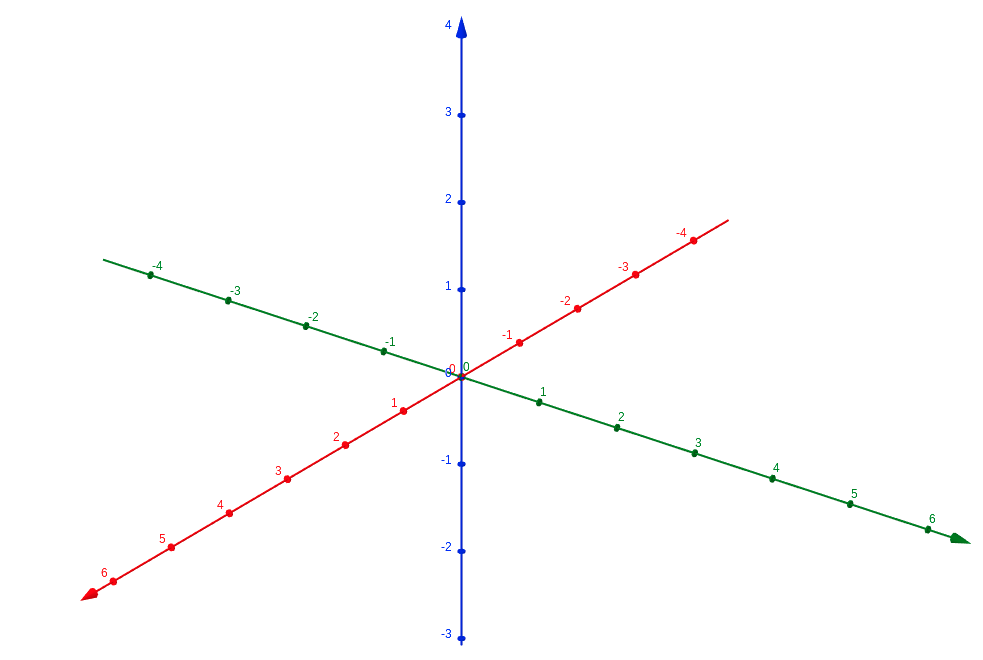
\includegraphics[scale=0.2]{figuras/eixos3d2.png}
\end{center}
\end{frame}


\begin{frame}[label=vetores]

\begin{exe}
\begin{enumerate}
\item Determine os pontos $(1,3,1)$ e $(3,-2,2)$ no sistema cartesiano.
\item Esboce o conjunto dos pontos que satisfazem a equação $z=3$.
\end{enumerate}
\end{exe}


\end{frame}


\begin{frame}[label=vetores]{Vetores no $\R^3$}
O conjunto $\R^3$ torna-se um espaço vetorial quando o munimos com as seguintes  operações: Se $\vec{u}=(u_1,u_2,u_3)$,  $\vec{v}=(v_1,v_2,v_2)$ e $\alpha\in \R$ então
\[\vec{u}+\vec{v}=(u_1+v_1,u_2+v_2,u_3+v_3),\]
\[\alpha \vec{v}=(\alpha v_1,\alpha v_2,\alpha v_3).\]
Neste caso, o {\color{blue}vetor nulo} é $\vec{0}=(0,0,0)$ e o {\color{blue}simétrico} de $\vec{v}$ é  $-\vec{v}=(-v_1,-v_2,-v_3)$.

\begin{center}
\begin{minipage}{0.7\textwidth}
\begin{block}{}
Se {\color{red}$A=(a_1,a_2,a_3)$} e {\color{red}$B=(b_1,b_2,b_3)$} então
\[{\color{red}\overrightarrow{AB}}={\color{blue}\vec{u}=(b_1-a_1,b_2-a_2,b_3-a_3)}.\]
\end{block}
\end{minipage}
\end{center}
\end{frame}


\begin{frame}[label=vetores]
Do mesmo modo,
\begin{center}
\begin{minipage}{0.7\textwidth}
\begin{block}{}
\[\|{\color{red}\overrightarrow{AB}}\|=\sqrt{{\color{blue}(b_1-a_1)^2+(b_2-a_2)^2 +(b_3-a_3)^2}}.\]
\end{block}
\end{minipage}
\end{center}


\begin{exe}
Dados $A=(0,3,1)$, $B=(2,3-1)$ e $C=(0,1,0)$ determine $2\vt{AB}+\vt{AC}$.
\end{exe}


\end{frame}

\subsection*{Vetores no $\R^n$}
\begin{frame}[label=vetores]{Vetores no $\R^n$}

De modo geral, denotamos por   $\R^n$ o conjunto formado pelas {\color{blue} $n$-uplas ordenadas} $(x_1,x_2,\ldots,x_n)$ tais $x_i\in \R$ para todo $i=1,2,\ldots,n$.
\medskip

O conjunto $\R^n$ torna-se um espaço vetorial quando o munimos com as seguintes  operações: Se $\vec{u}=(u_1,u_2,\ldots,u_n)$,  $\vec{v}=(v_1,v_2,\ldots,v_n)$ e $\alpha\in \R$ então
\[\vec{u}+\vec{v}=(u_1+v_1,u_2+v_2,\ldots,u_n+v_n),\]
\[\alpha \vec{v}=(\alpha v_1,\alpha v_2,\ldots,\alpha v_n).\]
Neste caso, o {\color{blue}vetor nulo} é $\vec{0}=(0,0,\ldots,0)$ e o {\color{blue}simétrico} de $\vec{v}$ é  $-\vec{v}=(-v_1,-v_2,\ldots,-v_n)$.

\begin{center}
\begin{minipage}{0.7\textwidth}
\begin{block}{}
Se {\color{red}$A=(a_1,a_2,\ldots,a_n)$} e {\color{red}$B=(b_1,b_2,\ldots,b_n)$} então
\[{\color{red}\overrightarrow{AB}}={\color{blue}\vec{u}=(b_1-a_1,b_2-a_2,\ldots,b_n-a_n)}.\]
\end{block}
\end{minipage}
\end{center}

\end{frame}

\begin{frame}[label=vetores]
De forma análoga, também definimos a {\color{blue} norma (ou comprimento)} de um vetor do $\R^n$ por
\begin{center}
\begin{minipage}{0.7\textwidth}
\begin{block}{}
Se {\color{blue}$\vec{u}=(u_1,u_2,\ldots,u_n)$} então
\[{\color{blue}\vec{u}=\sqrt{u_1^2+u_2^2+\ldots+u_n^2}}.\]
\end{block}
\end{minipage}
\end{center}

Um {\color{blue} vetor unitário} é um vetor que tem norma 1. Dado qualquer vetor não nulo $\vec{v}$, sempre podemos obter um {\color{blue}vetor unitário} $\vec{u}$ com mesmo sentido de $\vec{v}$, basta fazer
\[\vec{u}=\frac{1}{\|\vec{v}\|}\vec{v}.\]
Esse processo é chamada de {\color{blue} normalização} de $\vec{v}$. Alguns textos usam a notação $\hat{v}$ e o chamam de {\color{blue}versor}.


\end{frame}

\begin{frame}[label=vetores]


\begin{exe}
Normalize o vetor $\vec{v}=(2,-1,3)$.
\end{exe}


\begin{casa}
Normalize os vetores $\vec{u}=(1,\sqrt{2},\sqrt{3},0)$ e $\vec{v}=(4,-\sqrt{2},0,-5)$.
\end{casa}
\end{frame}

\begin{frame}[label=vetores]
Um nutricionista forneceu uma tabela que especifica a {\color{blue} quantidade mínima de cada tipo de vitamina que deve ser ingerida diariamente}.

\begin{center}

\begin{tabu}{|l|c|c|c|c|}
\hline
Tipo de vitamina & A & B & C & E\\ \hline
 Quantidade  mínima (mg) & 3 & 1.1 & 60 & 11\\ \hline
\end{tabu} 
\end{center}

Ele também forneceu uma tabela com a quantidade (em mg) de vitaminas em cada 100 gramas de 4 tipos de alimentos diferentes,
\begin{center}
\begin{tabu}{|c|c|c|c|c|}
\hline
& \multicolumn{4}{c|}{Alimento} \\ \hline
Vitamina & 1 & 2 & 3 & 4  \\ \hline
 \rowfont{\color{blue}} A &  0.140 & 0.580  & 0.150 & 0 \\ \hline
 \rowfont{\color{blue}} B &  0.08  & 0      & 1.30  & 0.08  \\ \hline
 \rowfont{\color{blue}} C &  0     & 0      & 26    & 38  \\ \hline
 \rowfont{\color{blue}} E & 1.60  & 0      & 6.90    & 0.2 \\ \hline
\end{tabu}
\end{center}

 Cada alimento é uma {\color{red}variável}, ou seja, 
\begin{center}
 $x_i$ representa a quantidade (em ``pacotes'' de 100g) do alimento $i$ que deve ser consumido diariamente, com $i=1,\ldots,4$. 
 \end{center}\bigskip

\end{frame}

\begin{frame}[label=vetores]
Com isso, se quisermos saber qual a quantidade de cada alimentos devemos consumir, para se ter a quantidade mínima de cada vitamina, devemos resolver o sistema:
\[
\begin{cases}
{\color{blue}0.14 } {\color{red}x_1}+ {\color{blue}0.58}{\color{red}x_2}+ {\color{blue}0.15}{\color{red}x_3}= 3,\\
{\color{blue}0.08}{\color{red}x_1}+{\color{blue}1.3}{\color{red}x_3}+{\color{blue}0.08}{\color{red}x_4}= 1.1,\\
{\color{blue}26}{\color{red}x_3}+{\color{blue}38}{\color{red}x_4}=  60,\\
{\color{blue}1.6}{\color{red}x_1}+{\color{blue}6.9}{\color{red}x_3}+{\color{blue}0.2}{\color{red}x_4}=  11,
\end{cases} 
\]
Usando a notação vetorial, temos:

\[
{\color{blue}
\begin{bmatrix}
0.14 \\ 0.08 \\ 0 \\ 1.60
\end{bmatrix}} {\color{red}x_1}+
{\color{blue}
\begin{bmatrix}
0.58 \\ 0 \\ 0 \\ 0
\end{bmatrix}} {\color{red}x_2}+
{\color{blue}
\begin{bmatrix}
0.150 \\ 1.30 \\ 26 \\ 6.90
\end{bmatrix}} {\color{red}x_3}+
{\color{blue}
\begin{bmatrix}
0\\ 0.08 \\ 38 \\ 0.2
\end{bmatrix}} {\color{red}x_4}=
\begin{bmatrix}
3 \\ 1.1\\ 60 \\ 11
\end{bmatrix}
\]
\end{frame}

\begin{frame}[label=vetores,fragile=singleslide]
\begin{pycode} 
import sympy as sp

x1,x2,x3,x4=sp.symbols('x_1 x_2 x_3 x_4',real=True)
X=sp.Matrix([x1,x2,x3,x4])
def pt(Y):
 return((Y[0],Y[1]))

v1=sp.Matrix([0.14,0.08,0,1.6])
v2=sp.Matrix([0.58,0,0,0])
v3=sp.Matrix([0.15,1.3,26,6.9])
v4=sp.Matrix([0,0.08,38,0.2])
B=sp.Matrix([3,1.1,60,11])

A=sp.Matrix.hstack(v1,v2,v3,v4)

AX=A*X
sol=sp.solve(sp.Eq(AX,B),(x1,x2,x3,x4))
\end{pycode} 
Aprenderemos mais à frente que este sistema tem a seguinte solução
\[x_1 \approx\pyl{sp.N(sol[x1],3)},\ x_2 \approx\pyl{sp.N(sol[x2],3)},\ x_3 \approx\pyl{sp.N(sol[x3],3)}\ \text{ e }\ x_4 \approx\pyl{sp.N(sol[x4],3)}.\]
Isto é, para se {\color{blue}ingerir a quantidade mínima de cada tipo de vitamina} devemos consumir:
\begin{center}

$\pyl{sp.N(sol[x1]*100,3)}$ gramas do alimento 1\\
$\pyl{sp.N(sol[x2]*100,3)}$ gramas do alimento 2\\
$\pyl{sp.N(sol[x3]*100,3)}$ gramas do alimento 3\\
$\pyl{sp.N(sol[x4]*100,3)}$ gramas do alimento 4
\end{center}
\end{frame}


\begin{frame}[label=vetores,fragile=singleslide]{Combinação Linear}

\begin{defin}
Um vetor $\vec{v}\in \R^n$ é uma {\color{blue} combinação linear} de vetores $\vec{v}_1, \vec{v}_2, \ldots, \vec{v}_k$ se existem escalares $\alpha_1,\alpha_2,\ldots, \alpha_k$ tais que
\[\vec{v}=\alpha_1\vec{v}_1+\alpha_2\vec{v}_2+\cdots +\alpha_k\vec{v}_k.\]
\end{defin}

\begin{pycode} 
import sympy as sp

x1,x2,x3,x4=sp.symbols('x_1 x_2 x_3 x_4',real=True)
X=sp.Matrix([x1,x2,x3,x4])
def pt(Y):
 return((Y[0],Y[1],Y[2],Y[3]))

v1=sp.Matrix([0.14,0.08,0,1.6])
v2=sp.Matrix([0.58,0,0,0])
v3=sp.Matrix([0.15,1.3,26,6.9])
v4=sp.Matrix([0,0.08,38,0.2])
B=sp.Matrix([3,1.1,60,11])
\end{pycode} 

No exemplo anterior, escrevemos  o vetor $\vec{v}=\pyl{B}$ como combinação linear dos vetores
\[\vec{v}_1=\pyl{v1},\ \vec{v}_2=\pyl{v2},\ \vec{v}_3=\pyl{v3},\ \text{ e } \vec{v}_4=\pyl{v4}. \]

\end{frame}

\section{Matrizes}

\subsection*{Matrizes}

\begin{frame}[label=matrizes]{Matrizes}

Uma {\color{blue} matriz} $A$, de tamanho $m\times n$, é uma tabela de $mn$ números dispostos em $m$ linhas e $n$ colunas, e será representada como:
\[
A=(a_{ij})_{m\times n}=\left[\begin{array}{cccc}
 a_{11}  & a_{12}  & \cdots &  a_{1n}  \\
 a_{21} & a_{22}  & \cdots  & a_{2n} \\
 \vdots & \vdots & \cdots & \vdots \\
 a_{m1} & a_{m2}  & \cdots  & a_{mn} \\
\end{array}\right]
\]

Dizemos que $a_{ij}$ é o {\color{blue} elemento} ou a {\color{blue} entrada} de posição $i,j$ da matriz $A$. Denotamos por $\mathbb{M}_{m\times n}(\R)$ o conjunto de todas as matrizes $m\times n$ cujos elementos são números reais.
\medskip

Quando $m=n$, dizemos que $A$ é uma {\color{blue} matriz quadrada de ordem n}. Neste caso, os elementos da $a_{11}, a_{22}, \ldots, a_{nn}$ formam {\color{blue}diagornal principal} de $A$.

\end{frame}

\begin{frame}[label=matrizes,fragile=singleslide]{Matrizes}
\begin{pycode}
import sympy as sp

A=sp.Matrix([[0, -1],[1, 0]])
B=sp.Matrix([[1,3,0],[2,-1,-3]])
\end{pycode}


\begin{exe} São exemplos de matrizes:
\[A=\py{sp.latex(A)},\ B=\py{sp.latex(B)}.\] 
\end{exe}


\end{frame}

\subsection*{Operações com matrizes}


\begin{frame}[label=matrizes,fragile=singleslide]{Soma de Matrizes}
\begin{pycode}
import sympy as sp

A=sp.Matrix([[1, 2,-3],[3, 4,0]])
B=sp.Matrix([[-2,1,5],[0,3,-4]])
C=A+B
\end{pycode}

A {\color{blue} soma} de duas matrizes de {\color{blue} mesmo tamanho} $A=(a_{ij})_{m\times n}$ e $B=(b_{ij})_{m\times n}$ é definida como sendo a matriz $m\times n$ $C=A+B$, obtida somando-se os elementos correspondentes de $A$ e $B$, ou seja, 
\[c_{ij}=a_{ij}+b_{ij},\]
para cada $i=1,\ldots,m$ e $j=1,\ldots,n$.

\begin{exe}
A soma das matrizes \[
A=\py{sp.latex(A)} \text{ e } \ 
B=\py{sp.latex(B)}
\]
é a matriz 
\[C=\py{sp.latex(C)}\]
\end{exe}
\end{frame}


\begin{frame}[label=matrizes,fragile=singleslide]{Multiplicação por escalar}
\begin{pycode}
import sympy as sp

A=sp.Matrix([[-2,1],[0,3],[5,-4]])
a=-3
B=a*A
\end{pycode}

A {\color{blue} multiplicação de uma matriz} $A=(a_{ij})_{m\times n}$  {\color{blue} por um escalar} $\alpha\in \R$ é definida como sendo a matriz $m\times n$, $B=\alpha A$, obtida multiplicando-se cada elemento da matriz $A$ pelo escalar $\alpha$, isto é,
\[b_{ij}=\alpha a_{ij},\]
para cada $i=1,\ldots,m$ e $j=1,\ldots,n$.



\end{frame}

\begin{frame}[label=matrizes]

\begin{exe}
A multiplicação  da matriz $A=\py{sp.latex(A)} $ pelo escalar $\alpha=\py{sp.latex(a)}$ é a matriz
\[B=\py{sp.latex(a)} A=\py{sp.latex(B)}.\]
\end{exe}

\begin{block}{}
Com a soma e a multiplicação por escalar, {\color{blue}o conjunto das matrizes $\mathbb{M}_{m\times n}(\R)$ forma um espaço vetorial}!
\medskip

Em particular, o conjunto das  matrizes linha ou das matrizes coluna formam o espaço vetorial $\R^n$.
\medskip

De agora em diante, não usaremos mais a notação $\vec{v}$ para representar um vetor. Escreveremos simplesmente $v$ e no contexto ficará claro que se trata de um vetor de $\R^n$.
\end{block}

\end{frame}

\begin{frame}[label=matrizes]{Produto de Matrizes}

Dadas duas matrizes $A=(a_{ij})_{{\color{blue}m}\times {\color{red}p}}$ e $B=(b_{ij})_{{\color{red}p}\times {\color{blue}n}}$, definimos o {\color{blue} produto de $A$ por $B$} como sendo a matriz $C=(c_{ij})_{{\color{blue}m\times n}}$, definida por
\[c_{ij}=\sum_{{\color{red}k=1}}^{n} a_{i{\color{red}k}}b_{{\color{red}k}j}
=a_{i{\color{red}1}}b_{{\color{red}1}j} +a_{i{\color{red}2}}b_{{\color{red}2}j} +\cdots + a_{i{\color{red}n}}b_{{\color{red}n}j},\]
para cada $i=1,\ldots,m$ e $j=1,\ldots,n$.

\begin{small}
\[
\left[
\begin{tabu}{cccc}
 a_{11}  & a_{12}  & \cdots &  a_{1p} \\
 \vdots & \vdots & \cdots & \vdots\\
\rowfont{\color{red}}  a_{i1} & a_{i2}  & \cdots  & a_{ip}\\
 \vdots & \vdots & \cdots & \vdots  \\
 a_{m1} & a_{m2}  & \cdots  & a_{mp}
\end{tabu}
\right]
\left[
\begin{tabu}{ccccc}
 b_{11}  & \cdots  &{\color{red} b_{1j} }& \cdots &  b_{1n} \\
 b_{21}  & \cdots  & {\color{red} b_{2j} } & \cdots &  b_{2n} \\
 \vdots & \cdots & {\color{red}\vdots} & \cdots & \vdots\\
 b_{p1} & \cdots  & {\color{red} b_{pj} } & \cdots & b_{pn}
\end{tabu}
\right]
=
\left[
\begin{tabu}{ccc}
 c_{11}  &  \cdots &  c_{1n} \\
 \vdots &   {\color{red}c_{ij}} & \vdots\\
 c_{m1} & \cdots   &   c_{mn}
\end{tabu}
\right]
\]
\end{small}

\end{frame}

\begin{frame}[label=matrizes,fragile=singleslide]
\begin{pycode}
import sympy as sp

A=sp.Matrix([[1,2,-3],[3,4,0]])
B=sp.Matrix([[-2,1,0],[0,3,1],[5,-4,0]])
C=A*B
\end{pycode}

\begin{exe}
Considere as matrizes  $A=\py{sp.latex(A)} $ e $B=\py{sp.latex(B)} $. Então,
\[AB=\py{sp.latex(C)}.\]
\end{exe}
\end{frame}


\begin{frame}[label=matrizes]{Transformações Lineares}
Uma matriz $A$, de ordem $m\times n$, pode ser interpretada como uma {\color{blue}transformação} que leva vetores de $\R^n$ em vetores $\R^m$.

\begin{exer}
\begin{enumerate}
\item  A matriz 
$R=\begin{bmatrix}
0 & -1\\ 1 & 0 
\end{bmatrix}$ rotaciona qualquer vetor do plano $90^\circ$ no sentido anti-horário. Verifique esboçando no plano os vetores $v=\begin{bmatrix}
1\\ 1
\end{bmatrix}$ e $u=Rv$.

\item A matriz $S=\begin{bmatrix}
0 & 1\\ 1 & 0 
\end{bmatrix}$ reflete um vetor em relação à reta $y=x$. Verifique esboçando no plano os vetores $u$ do item anterior e o vetor  $w=Su$.
\end{enumerate}
\end{exer}


\end{frame}


\begin{frame}[label=matrizes]
Neste sentido, o {\color{blue}produto de matrizes} desempenha o papel de composição de funções.
\begin{exer}
Verifique isso calculando a matriz $M=SR$, onde $R$ e $S$ são as matrizes do exercício anterior e esboce os vetores $u$ e $Mu$.
\end{exer}


\end{frame}


\begin{frame}[label=matrizes,fragile=singleslide]
\begin{pycode}
import sympy as sp

R=sp.Matrix([[0,-1],[1,0]])
S=sp.Matrix([[0,1],[1,0]])
A=sp.Matrix([0,1])
B=sp.Matrix([1,1])
C=sp.Matrix([1,3])


\end{pycode}

\begin{casa}
Considere as matrizes  $R=\py{sp.latex(R)} $ e $S=\py{sp.latex(S)} $, e os vetores $u=\pyl{A}$, $v=\pyl{B}$ e $w=\pyl{C}$
\begin{enumerate}

\item Esboce o triângulo $ABC$ que tem como vértices as extremidades dos vetores.

\item Calcule $u'=Ru$, $v'=Rv$ e $w'=Rw$. Esboce o novo  triângulo $A'B'C'$ com vértices dados pelos novos vetores.

\item Calcule $u''=Su'$, $v''=Sv'$ e $w''=Sw'$. Esboce o triângulo $A''B''C''$ com vértices dados pelos novos vetores.

\item Calcule $M=SR$. Esboce o triângulo com vértices em $Mu$, $Mv$ e $Mw$.
\end{enumerate}
\end{casa}
\end{frame}





\begin{frame}[label=Matrizes]
\begin{casa}
Sejam 
$A=\begin{bmatrix}
1 & 2 \\
3 & 4
\end{bmatrix} $ e 
$B=\begin{bmatrix}
-2 & 1 \\
0 & 3
\end{bmatrix} $.
Calcule $AB$ e $BA$. 
\end{casa}
\end{frame}


\subsection*{Propriedades das Matrizes }

\begin{frame}[label=matrizes]{Propriedades das operações com Matrizes}

Sejam $A, B$ e $C$ matrizes com tamanhos apropriados e $\alpha,\beta\in \R$. São válidas as seguintes propriedades:

\begin{enumerate}
\item $A+B=B+A$ (comutatividade da soma)
\item $A+(B+C)=(A+B)+C$ (associatividade da soma)
\item $\alpha(\beta A)=(\alpha \beta)A$ (associatividade do produto por escalar)
\item $(\alpha+\beta)A=\alpha A+\beta A$ (distributividade do produto por escalar)
\item $\alpha(A+B)=\alpha A+\alpha B$ (distributividade do produto por escalar)
\item $A(BC)=(AB)C$ (associatividade do produto)
\item $A(B+C)=AB+AC$ e $(B+C)A=BA+CA$ (distributividade)
\end{enumerate}


\end{frame}


\begin{frame}
\begin{exe}
Se $A$ e $B$ são matrizes quadradas, então vale a identidade? \[(A+B)(A-B)=A^2-B^2.\]
\end{exe}
\end{frame}


\subsection*{Matriz Identidade}
\begin{frame}[label=matrizes]{Matriz Identidade}

A matriz $n\times n$, definida por
\[I_n=\begin{bmatrix}
1 & 0 & \cdots & 0\\
0 & 1 & \cdots & 0\\
\vdots & \vdots & \ddots & \vdots\\
0 & 0 & \cdots & 1
\end{bmatrix},\]
chamada {\color{blue} matriz identidade} é o \textbf{elemento neutro da multiplicação}, isto é, 
\[AI_n=I_mA=A,\]
para toda matriz $A=(a_{ij})_{m\times n}$.



\end{frame}





\subsection*{Transposta}
\begin{frame}[label=matrizes,fragile=singleslide]{Matriz Transposta}

A {\color{blue} transposta} de uma matriz $A=(a_{ij})_{{\color{blue}m}\times {\color{red}n}}$, denotada por $A^t$,  é a matriz obtida a partir de $A$ trocando-se as linhas com as colunas, isto é,  $A^t=(b_{ij})_{{\color{red}n}\times {\color{blue}m}}$, onde
\[b_{ij}=a_{ji},\]
para cada $i=1,\ldots,m$ e $j=1,\ldots,p$.


\begin{pycode}
import sympy as sp

A=sp.Matrix([[1,2,-3],[3,4,0]])
B=A.T
\end{pycode}

\begin{exe}
A transposta da matriz  $A=\py{sp.latex(A)} $ é a matriz 
\[A^t=\py{sp.latex(B)}.\]
\end{exe}

\end{frame}




\begin{frame}[label=matrizes,fragile=singleslide]{Propriedades da Transposta}

Sejam $A$ e $B$ matrizes com tamanhos apropriados e $\alpha,\in \R$. São válidas as seguintes propriedades:

\begin{enumerate}
\item $(A^t)^t=A$ 
\item $(A+B)^t=A^t+B^t$
\item $(\alpha A)^t=\alpha A^t$
\item $(AB)^t=B^tA^t$
\end{enumerate}

\end{frame}

\begin{frame}
\begin{casa}
\begin{enumerate}
\item Sejam    $A=\begin{bmatrix} x & 4 &  -2 \end{bmatrix}$  e  $B=\begin{bmatrix} 2 & -3 & 5 \end{bmatrix}$. Encontre o valor de $x$ tal que $AB^t=0,$ onde $0$ é a matriz nula, isto é, com todas as entradas sendo zero.

\item Calcule $M^3$, onde 
\[M=\begin{bmatrix}
0 & 1 & 0\\
0 & 0 & 1\\
0 & 0 & 0
\end{bmatrix}.
\]
\end{enumerate}
\end{casa}
\end{frame}

\subsection*{Usando o sympy para operar matrizes}



\begin{frame}[label=matrizes,fragile=singleslide]{Operações com matrizes usando o sympy}
	\begin{footnotesize}
\begin{pyverbatim}
import sympy as sp

A=sp.Matrix([[1, 2,-3],[3, 4,0]])
B=sp.Matrix([[-2,1,5],[0,3,-4]])
C=sp.Matrix([[-2,1,0],[0,3,0],[5,-4,0]])
S=A+B
display(S)
P=A*C
display(P)
T=A.T
display(T)

\end{pyverbatim}
	\end{footnotesize}		
\begin{pycode}
import sympy as sp

A=sp.Matrix([[1, 2,-3],[3, 4,0]])
B=sp.Matrix([[-2,1,5],[0,3,-4]])
C=sp.Matrix([[-2,1,0],[0,3,1],[5,-4,0]])
S=A+B
P=A*C
T=A.T
\end{pycode}
\[A=\pyl{A},\ B=\pyl{B},\ C=\pyl{C}\]

\[A+B=\pyl{S},\ AC=\pyl{P},\ A^t=\pyl{T}\]

\end{frame}






\section{Produto Escalar}

\subsection*{O Produto Escalar}

\begin{frame}[label=vetores2]{O produto escalar}

\begin{defin}
Dados dois vetores $u=(u_1,u_2,\ldots,u_n)$ e $v=(v_1,v_2,\ldots,v_n)$ do $\R^n$, definimos o {\color{blue} produto escalar (ou produto interno)} entre eles por:
\[u\cdot v=u_1v_1+u_2v_2+\cdots+ u_nv_n.\]
\end{defin}

\begin{exe}
Calcule $u\cdot v$, em que $u=(1,2,-3)$ e $v=(-3,5,2)$.
\end{exe}

\end{frame}

\begin{frame}[label=vetores2]

\begin{block}{Propriedades do produto interno} Para quaisquer vetores $u$, ${v}$ e ${w}$ em $\R^n$ e para qualquer número real $\lambda$, valem as propriedades:
			
			\begin{enumerate}
				\item ${u}\cdot {v}={v}\cdot{u}$;
				\item $\lambda( {u}\cdot {v})=(\lambda  {u})\cdot {v}=  {u}\cdot(\lambda {v});$
				\item $( {u}+ {v})\cdot {w}= {u}\cdot {w}+ {v}\cdot {w}$;
				\item $ {u}\cdot {u}=\n{ {u}}^2$.
%				\item $| {u}\cdot {v}|\leq \n{\vect{u}}\n{\vect{v}}$ (desigualdade de Cauchy-Schwartz)
			\end{enumerate}            
		\end{block}
\begin{exe}
Mostre que
\[\|u-v\|^2=\|u\|^2-2u\cdot v+\|v\|^2.\]
\end{exe}

\end{frame}

\subsection*{Ângulo entre vetores}
\begin{frame}[label=vetores2]{Ângulo entre vetores no $\R^2$ e $\R^3$}
	\begin{defin}[ângulo entre vetores] Dados dois vetores $\vt{u}$ e $\vt{v}$, no $\R^2$ ou $\R^3$, definimos o \dest{ângulo entre $\vt{u}$ e $\vt{v}$} como sendo o menor ângulo formado por seus respectivos representantes com mesma origem.			
		\end{defin}

\begin{center}
\begin{minipage}{0.4\textwidth}
	\begin{tikzpicture}
	\tikzset{>=latex}
	\coordinate (O) at (0,0);
	\coordinate (A) at (1,2);
	\coordinate (B) at (2,0);
	\coordinate (C) at (4,1);
	
	\coordinate (X) at (3,0);
	
	\draw[->,ultra thick] (O) -- (A);
	\node[left] at (A) {$\vect{v}$};
	\draw[->,ultra thick] (O) -- (B);
	\node[below] at (B) {$\vect{u}$};
	
	\pic[draw]{angle = B--O--A};
	\node at (0.7,0.5) {$\theta$};
	

	\end{tikzpicture}
\end{minipage}
\begin{minipage}{0.4\textwidth}
	\begin{tikzpicture}
	\tikzset{>=latex}
	\coordinate (O) at (0,0);
	\coordinate (A) at (-1,-2);
	\coordinate (B) at (2,0);
	
	
	\draw[->,ultra thick] (O) -- (A);
	\node[left] at (A) {$\vect{v}$};
	\draw[->,ultra thick] (O) -- (B);
	\node[above left] at (B) {$\vect{u}$};
	
	\pic[draw]{angle = A--O--B};
	\node at (0.6,-0.6) {$\theta$};

	
	\end{tikzpicture}
\end{minipage}

\end{center}
\end{frame}

\begin{frame}
\begin{prop}Dados  $\vt{u}$ e $\vt{v}$, no $\R^2$ ou $\R^3$, então
		\[\vt{u}\cdot\vt{v}=\n{\vt{u}}\n{\vt{v}}\cos ({\color{red}\theta}),\]
		onde ${\color{red}\theta}$ é o ângulo entre eles.
		
	\end{prop}

\begin{center}
	\begin{minipage}{0.3\textwidth}
		\begin{tikzpicture}
		\tikzset{>=latex}
		\coordinate (O) at (0,0);
		\coordinate (A) at (1,2);
		\coordinate (B) at (2,0);
		\coordinate (C) at (4,1);
		
		\coordinate (X) at (3,0);
		
		\draw[->,ultra thick] (O) -- (A);
		\draw[->,ultra thick] (O) -- (B);
		
		\pic[draw]{angle = B--O--A};
		\node at (0.7,0.5) {${\color{red}\theta}$};
		
		\node at (1,-.5) {$\vect{u}\cdot\vect{v}>0$};
		\end{tikzpicture}
	\end{minipage}
	\begin{minipage}{0.3\textwidth}
		\begin{tikzpicture}
		\tikzset{>=latex}
		\coordinate (O) at (0,0);
		\coordinate (A) at (-1,2);
		\coordinate (B) at (2,0);
		
		
		\draw[->,ultra thick] (O) -- (A);
		\draw[->,ultra thick] (O) -- (B);
		
		\pic[draw]{angle = B--O--A};
		\node at (0.7,0.5) {${\color{red}\theta}$};
		\node at (1,-.5) {$\vect{u}\cdot\vect{v}<0$};
		
		\end{tikzpicture}
	\end{minipage}
	\begin{minipage}{0.3\textwidth}
		\begin{tikzpicture}
		\tikzset{>=latex}
		\coordinate (O) at (0,0);
		\coordinate (A) at (0,2);
		\coordinate (B) at (2,0);
		
		
		\draw[->,ultra thick] (O) -- (A);
		\draw[->,ultra thick] (O) -- (B);
		
		\draw (0.5,0) -- (0.5,.5) -- (0,0.5);
		\draw[fill] (0.25,.25) circle (1pt);
		\node at (0.7,0.5){${\color{red}\theta}$};
		\node at (1,-.5) {$\vect{u}\cdot\vect{v}=0$};
		\end{tikzpicture}
	\end{minipage}
\end{center}

\end{frame}

\subsection*{Lei dos Cossenos}
\begin{frame}[label=vetores2]


	\begin{exampleblock}{Lei dos Cossenos}
	Seja $ABC$ um triângulo qualquer com lados ${\color{red}a}, {\color{blue}b}$ e ${\color{blue}c}$, então
	\[{\color{red}a^2}={\color{blue}b^2}+{\color{blue}c^2}-2{\color{blue}b c}\cos( {\color{red}\hat{A}}),\]
	onde ${\color{red}\hat{A}}$ é o ângulo oposto ao lado $a$. 
	
	\begin{center}
		\begin{tikzpicture}
		\draw[thick,blue] (0,0) -- (2,1) ;
		\draw[thick,red] (2,1) -- (3,0) ;
		\draw[thick,blue] (3,0) -- (0,0);
		\node[left] at (0,0) {$A$};
		\node[above] at (2,1) {$B$};
		\node[right] at (3,0) {$C$};
		\node at (2.8,0.7) {${\color{red}a}$};
		\node at (1,1) {${\color{blue}c}$};
		\node at (1.5,-0.3) {${\color{blue}b}$};
		\draw[red] (0.5,0) arc (0:14:1cm);
		\node at (0.8,0.2) {${\color{red}\hat{A}}$};
		\end{tikzpicture}
	\end{center}
\end{exampleblock}
\end{frame}



\begin{frame}[label=vetores2]
\begin{exe}
Determine os ângulo entre os vetores
\begin{enumerate}
\item $\vec{u}=(1,0)$ e $\vec{v}=(\sqrt{3},1)$.

\item $\vec{u}=(2,0,1)$ e $\vec{v}=(1,-2,-1)$.
\end{enumerate}
\end{exe}

\begin{defin}
Dados vetores $u$ e $v$ em $\R^n$, definimos o {\color{blue}ângulo entre $u$ e $v$} como sendo o valor $0\leq \theta\leq \pi$ que satisfaz:
\[\cos(\theta)=\frac{u\cdot v}{\|u\|\, \|v\|}. \] 
\end{defin}

Dizemos que dois vetores são {\color{blue}ortogonais} quando o ângulo entre eles é de $90^\circ$, isto é, quando 
\[u\cdot v=0.\]
\end{frame}


\begin{frame}[label=vetores2]
\begin{casa}
\begin{enumerate}
\item Determine o ângulo entre os vetores $\vec{u}=(2,-3)$ e $\vec{v}=(1,1)$.
\item Um retângulo tem vértices nos pontos $A=(1,2,3)$, $B=(3,6,-2)$ e $C=(0,5,-4)$. Determine o ponto $D$.
\end{enumerate}
\end{casa}
\end{frame}


\subsection*{Produto escalar usando o sympy}
\begin{frame}[label=vetores2,fragile=singleslide]{Produto escalar usando o sympy}

	\begin{footnotesize}
\begin{pyverbatim}
import sympy as sp
import mpmath

u=sp.Matrix([1.12,-3.25,2.07,-1.83 ])
v=sp.Matrix([-2.29,1.72,4.33,-1.54])
uv=u.dot(v)
nu=u.norm()
nv=v.norm()
cos=uv/(nu*nv)
theta=sp.acos(cos)
thetag=round(mp.degrees(theta),2)
\end{pyverbatim}
	\end{footnotesize}	

\begin{pycode}
import sympy as sp
import mpmath as mp

u=sp.Matrix([1.12,-3.25,2.07,-1.83 ])
v=sp.Matrix([-2.29,1.72,4.33,-1.54])
uv=u.dot(v)
nu=u.norm()
nv=v.norm()
cos=uv/(nu*nv)
theta=sp.acos(cos)
thetag=round(mp.degrees(theta),2)
\end{pycode}
Denotando-se os vetores como matrizes colunas, temos:
\[u\cdot v=\pyl{u}\cdot \pyl{v}=\pyl{uv}\]
\[\cos(\theta)\approx\pyl{cos}\Rightarrow \theta\approx\pyl{theta} \text{ rad}\approx \pyl{thetag}^\circ.\]
\end{frame}





\section{Retas e Planos}

\subsection*{Equação Paramétrica da Reta}


\begin{frame}[label=retas]{Equação Paramétrica de uma Reta}

Fixados um ponto ${\color{red} A}$ de uma reta $r$ e um vetor ${\color{blue}\vec{v}}$ paralelo a esta reta, podemos descrever os pontos $P$ dessa reta da seguinte forma:
\[P={\color{red}A}+t{\color{blue}\vec{v}},\ t\in \R.\]
	\begin{center}
		\begin{tikzpicture}
		\tikzset{>=latex}
		\draw[thick] (-1,-1) -- (2,2);
		\node[left] at (2,2) {r};
		\draw[fill=red] (0,0) circle [radius=1.5pt];
		\node[above left] at (0,0) {$\textcolor{red}{A}$};
		\draw[thick, blue,->] (2,0) -- (0.7+2,0.7);
		\node[blue, right] at (0.7+2,0.7) {$\vec{v}$};
		\onslide<2->{
		\draw[fill=black] (1.5,1.5) circle [radius=1.5pt];
		\node[above left] at (1.5,1.5) {$P$};}
	
	\onslide<3->{
\draw[thick, blue,->] (0,0) -- (1.5,1.5);	
  }
		\end{tikzpicture}
	\end{center}
	
Esta equação é dita {\color{blue} equação vetorial paramétrica da reta $r$}, $t$ é dito ser um {\color{blue}parâmetro} e ${\color{blue}\vec{v}}$ é chamado de {\color{blue}vetor diretor.}

\end{frame}

\begin{frame}[label=retas]
Se	$P=(x,y)$, $\textcolor{red}{A=(x_0,y_0)}$ e $\textcolor{blue}{\vt{v}=(a,b)}$
em coordenadas temos que
\[	\left\{\begin{array}{l}
	x=\textcolor{red}{x_0}+\textcolor{blue}{a}t\\
	y=\textcolor{red}{y_0}+\textcolor{blue}{b}t,\  t\in \R.
	\end{array}\right.\]


Analogamente, se 	$P=(x,y,z)$, $\textcolor{red}{A=(x_0,y_0,z_0)}$ e $\textcolor{blue}{\vt{v}=(a,b,c)}$
		\[	\left\{\begin{array}{l}
		x=\textcolor{red}{x_0}+\textcolor{blue}{a}t\\
		y=\textcolor{red}{y_0}+\textcolor{blue}{b}t\\
		z=\textcolor{red}{z_0}+\textcolor{blue}{c}t,\  t\in \R.
		\end{array}\right.\]
		Estas equações são chamadas simplesmente de \dest{equações paramétricas  da reta} $r$.


\end{frame}

\begin{frame}[label=retas]
	\frametitle{ }
	%\begin{scriptsize}
	{\begin{exe}\label{exer4} \noindent
			
			\begin{enumerate}[a]
				\item Determine as equações paramétricas da reta que passa pelos pontos  $A=(-1,0)$ e $B=(0,1)$ .
				
				\item Determinar  as equações paramétricas da reta $r$ que passa pelos
				pontos $A = (1, 2, -2)$ e $B = (-1, 4, 2)$.

	\item\label{ex6} Sejam $A=(0,1,8), B=(-3,0,9)$ e $r: X=(1,2,0)+t(1,1,-3)$. Determine o ponto $C$ de $r$ tal que $A,B$ e $C$ sejam vértices de um triângulo retângulo com ângulo reto no vértice $A$.
			\end{enumerate}
	\end{exe}}

\end{frame}

\begin{frame}[label=retas]
	\begin{casa}
	\begin{enumerate}
		\item 	Considere os pontos $A = (2, -1, 0)$,  $B  = (0, 1, -1)$. Determine
	 a reta $r$ que passa por $A$ e $B$.

	\item Sejam $A=(0,1,8), B=(-3,0,9)$ e $r: X=(1,2,0)+t(1,1,-3)$. Determine o ponto $C$ de $r$ tal que $A,B$ e $C$ sejam vértices de um triângulo retângulo com ângulo reto no vértice $C$. 
	\end{enumerate}
	
	\end{casa}

	
\begin{center}
\begin{block}{}
Note que a equação vetorial paramétrica da reta é válida para qualquer dimensão!
\end{block}
\end{center}
\end{frame}

\subsection*{Equações Cartesianas da reta em $\R^2$}
\begin{frame}[label=retas]{Equação Cartesiana da reta em $\R^2$}
	Fixe um ponto $\textcolor{red}{A=(x_0,y_0)}$ de uma reta $r$ e seja  $\textcolor{blue}{\vt{v}=(a,b)}$ um vetor ortogonal a esta reta. 
	
		\begin{center}
		\begin{tikzpicture}
		\tikzset{>=latex}
		\draw[thick] (-1,-1) -- (2,2);
		\node[left] at (2,2) {r};
		
		\draw[thick, blue,->] (1,0.5) -- (0.7+1,-0.7+0.5);
		\node[blue, right] at (0.7+1,-0.7+0.5) {$\vec{v}$};
		\draw[fill=red] (0,0) circle [radius=1.5pt];
		\node[above left] at (0,0) {$\textcolor{red}{A}$};
		\onslide<1->{
			
			\draw[fill=black] (1.5,1.5) circle [radius=1.5pt];
			\node[above left] at (1.5,1.5) {$P$};}
		
		\onslide<1->{
			\draw[thick, red,->] (0,0) -- (1.5,1.5);	
		}
		\end{tikzpicture}
	\end{center}
	
Dado um ponto qualquer   $P=(x,y)$	desta reta $r$  temos que
		\[	\textcolor{blue}{a}x+\textcolor{blue}{b}y+c=0.\]
Esta equação é dita \dest{equação cartesiana da reta}.
\end{frame}
	
\begin{frame}[label=retas]
	\begin{exe}\noindent
  Encontre a equação cartesiana da reta que passa pelos pontos $P=(1,3)$ e $Q=(5,-9)$.
	\end{exe}

	\begin{block}{Equação reduzida da reta}
		A equação cartesiana de uma reta é chamada de   \dest{equação reduzida} quando  está na seguinte forma:
		\[y=mx+n.\]
		O coeficiente  $m$ é dito \dest{coeficiente angular} da reta e mede a tangente do ângulo que a reta faz com o eixo $OX$. E o número $n$ é dito \dest{coeficiente linear} da reta e representa a ordenada do ponto de interseção da reta com o eixo $OY$.
	\end{block}

\end{frame}

\begin{frame}
	
	%\begin{scriptsize}
	\begin{block}{Equação segmentária da reta}
		A equação cartesiana de uma reta é chamada de   \dest{equação segmentária}  quando  está na seguinte forma:
		\[\frac{x}{p}+\frac{y}{q}=1.\]
		Neste caso, a reta intercepta os eixos $OX$ e $OY$ nas coordenadas $p$ e $q$ respectivamente. 
	\end{block}
	
	%\end{scriptsize}
\end{frame}

\begin{frame}
	\begin{exe}
	\begin{enumerate}
		\item 	 Determine a equação cartesiana da reta $r$ que passa pelos pontos $A=(0,3)$ e $B=(2,0)$.
		
		
		\item Determine a equação cartesiana da reta que passa pelos pontos $A=(0,1)$ e $B=(2,2)$.
		
		
	\end{enumerate}
	\end{exe}


	\begin{minipage}{0.45\textwidth}
		\begin{figure}[h]
		\begin{tikzpicture}[scale=0.8]
	\tikzset{>=latex}
	\draw[help lines, color=gray!70, dashed] (0,0) grid (2,3);
	\draw[->,thick] (0,0)--(2.5,0) node[right]{$OX$};
	\draw[->,thick] (0,0)--(0,3.5) node[above]{$OY$};
	\foreach \i in {1,...,2}
	\node[below,scale=0.7] at (\i,0) {$\i$};
	\foreach \i in {1,...,3}
	\node[left,scale=0.7] at (0,\i) {$\i$};
	
	
	\coordinate (O) at (0,0);
	\coordinate (A) at (0,3);
	\coordinate (B) at (2,0);
	
	
	\node[blue] at (A) {\textbullet};
	\node[blue,right] at (A) {$A$};
	
	\node[blue] at (B) {\textbullet};
	\node[blue,above] at (B) {$B$};
	
	\draw[blue,thick] (-.5,3.75) -- (2.5,-0.75) ;
	
	
	
	%	\node[blue] at (Q) {\textbullet};
	%	\node[blue,above] at (Q) {$Q$};
	
	\end{tikzpicture}
	\caption{Exemplo 1}
	\end{figure}
	\end{minipage}
	\begin{minipage}{0.45\textwidth}
		\begin{figure}[h]
	\begin{tikzpicture}[scale=0.8]
	\tikzset{>=latex}
	\draw[help lines, color=gray!70, dashed] (0,0) grid (2,2);
	\draw[->,thick] (0,0)--(2.5,0) node[right]{$OX$};
	\draw[->,thick] (0,0)--(0,2.5) node[above]{$OY$};
	\foreach \i in {1,...,2}
	\node[below,scale=0.7] at (\i,0) {$\i$};
	\foreach \i in {1,...,2}
	\node[left,scale=0.7] at (0,\i) {$\i$};
	
	
	\coordinate (O) at (0,0);
	\coordinate (A) at (0,1);
	\coordinate (B) at (2,2);
	
	
	\node[blue] at (A) {\textbullet};
	\node[blue,right] at (A) {$A$};
	
	\node[blue] at (B) {\textbullet};
	\node[blue,above] at (B) {$B$};
	
	\draw[blue,thick] (-.5,0.75) -- (2.5,2.25) ;
	
	
	
	%	\node[blue] at (Q) {\textbullet};
	%	\node[blue,above] at (Q) {$Q$};
	
	\end{tikzpicture}
	\caption{Exemplo 2}
\end{figure}
	\end{minipage}


\end{frame}

\begin{frame}[label=retas]
\begin{casa}
	\begin{enumerate}
		\item Determine a equação da reta que passa pelo ponto $A=(3,-5)$ e tem coeficiente angular igual a $5$.
		
		\item Esboce no plano a reta cuja equação é dada por $\frac{x}{-3}+\frac{y}{2}=1$.
	\end{enumerate}
\end{casa}
\end{frame}

\subsection*{Equação Cartesiana do Plano no Espaço}

\begin{frame}[label=planos]{Equação Cartesiana do Plano no Espaço}
Sejam  ${\color{red}A=(x_0,y_0,z_0)}$  um ponto de um plano em $\R^3$, $\textcolor{blue}{\vt{n}=(a,b,c)}\perp \pi$, então os pontos e  $P=(x,y,z)$do plano devem satisfazer a seguinte \dt{equação cartesiana}
\[{\color{blue}a}x+{\color{blue}b}y+{\color{blue}c}z+{\color{red}d}=0\]
\begin{center}
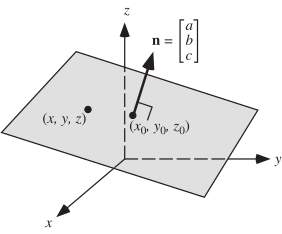
\includegraphics[scale=0.8]{figuras/normal-vector.png}
\end{center}
\end{frame}

\begin{frame}
\begin{exe}
Determine a equação do plano que passa pelo ponto $A=(1,0,1)$ e é perpendicular à reta
$r: X=(-1,1,2)+t(0,2,1),\ t\in \R$.
\end{exe}

\end{frame}

\begin{frame}[label=sistemas,fragile=singleslide]{Interseção de Planos}

\begin{pycode}
import sympy as sp

x,y,z=sp.symbols('x y z',real=True)
X=sp.Matrix([x,y,z])
A=sp.Matrix([[2, -1,1],[1,3,4]])
B=sp.Matrix([2,1])
AX=A*X
eq1=sp.Eq(AX[0],B[0])
eq2=sp.Eq(AX[1],B[1])

sol=sp.solve(sp.Eq(AX,B),(x,y,z))

\end{pycode}


Qual o conjunto dos pontos do espaço que estão na interseção dos dois planos a seguir?

\[\begin{cases}
\pyl{eq1}\\
\pyl{eq2}
\end{cases}\]
Para descobrir isso, vemos multiplicar a 2\fm equação por $-2$ e somar com a primeira.
\[\begin{cases}
\pyl{eq1}\\
\pyl{-2*AX[1]+AX[0]}=\pyl{-2*B[1]+B[0]}
\end{cases}\]
Note que geometricamente os dois sistemas tratam de interseção de planos diferentes, mas algebricamente os sistemas são {\color{blue} equivalentes}, isto é, têm o mesmo conjunto de pontos $(x,y,z)$ como solução. Entretanto o segundo sistema é mais simples!
\end{frame}


\begin{frame}[label=sistemas,fragile=singleslide]

\begin{pycode}
import sympy as sp

x,y,z=sp.symbols('x y z',real=True)
X=sp.Matrix([x,y,z])
A=sp.Matrix([[2, -1,1],[1,3,4]])
B=sp.Matrix([2,1])
AX=A*X
eq1=sp.Eq(AX[0],B[0])
eq2=sp.Eq(AX[1],B[1])

sol=sp.solve(sp.Eq(AX,B),(x,y,z))

\end{pycode}

\[\begin{cases}
\pyl{eq1}\\
\pyl{-2*AX[1]+AX[0]}=\pyl{-2*B[1]+B[0]}
\end{cases}\]
É fácil ver que este sistema tem soluções da forma:
\[y=\pyl{sol[y]} \text{ e } x=\pyl{sol[x]}.\]
Fazendo $z=t$, vemos que os pontos da interseção são da forma
\[X=(1-t,-t,t)=(1,0,0)+t(-1,-1,1)\ t \in \R,\]
isto é, uma reta em $\R^3$. 
\medskip

Isto nos motiva a estudar os chamados {\color{blue}sistemas lineares}.

\end{frame}











\section{Sistema de Equações Lineares}


\begin{frame}[label=sistemas]{Sistemas de Equações Lineares}

Uma {\color{blue} equação linear} em {\color{red}$n$} variáveis {\color{red} $x_1,x_2,\ldots, x_n$} é uma equação da forma
\[{\color{blue}a_1}{\color{red}x_1}+{\color{blue}a_2}{\color{red}x_2}+\cdots+{\color{blue}a_n}{\color{red}x_n}=b,\]
em que {\color{blue} $a_1,a_2,\ldots, a_n$} e $b$ são constantes reais.

Um {\color{blue}sistema  de $m$ equações lineares} a {\color{red}$n$ incógnitas} é um conjunto de {\color{blue}$m$} equações lineares, isto é,
\[
\left\{\begin{matrix}
 {\color{blue}a_{11}}{\color{red}x_1} & + &  {\color{blue}a_{12}}{\color{red}x_2} & + & \cdots & + & {\color{blue}a_{1n}}{\color{red}x_n} & = & b_1  \\
 {\color{blue}a_{21}}{\color{red}x_1} & + & {\color{blue}a_{22}}{\color{red}x_2} & + &   \cdots & + & {\color{blue}a_{2n}}{\color{red}x_n} & = & b_2  \\
\vdots & \vdots  & & & &  & \vdots & \vdots & \vdots  \\
 {\color{blue}a_{m1}}{\color{red}x_1} & + & {\color{blue}a_{m2}}{\color{red}x_2} & + &  \cdots  & + &   {\color{blue}a_{mn}}{\color{red}x_n} & = & b_m. 
\end{matrix}
\right.
\]
em que {\color{blue}$a_{ij}$} e $b_k$ são constantes reais, para $i,k=1,\ldots,m$ e $j=1,\ldots,n$.


\end{frame}


\begin{frame}[label=sistemas]{Sistemas de Equações Lineares}

Usando o produto matricial, o {\color{blue}sistema linear} pode ser escrito da seguinte forma
\[
{\color{blue} \underbrace{\begin{bmatrix}
 a_{11}  & a_{12}  & \cdots &  a_{1n}  \\
 a_{21} & a_{22}  & \cdots  & a_{2n} \\
 \vdots & \vdots & \cdots & \vdots \\
 a_{m1} & a_{m2}  & \cdots  & a_{mn} 
\end{bmatrix}}_{A}}\ \
{\color{red}
\underbrace{\begin{bmatrix}
x_1\\ x_2\\ \vdots \\ x_n
\end{bmatrix}}_{X}
}
=
\underbrace{\begin{bmatrix}
b_1 \\ b_2\\ \vdots \\ b_n
\end{bmatrix}}_{B}.
\]

\end{frame}

\begin{frame}[label=sistemas]{Solução de um Sistema Linear}
Uma {\color{blue} solução} de um sistema linear a $n$ incógnitas é um vetor
$(s_1,s_2,\ldots,s_n)\in \R^n$ que satisfaz a equação matricial $AX=B$ associada ao sistema. O conjunto de todas as soluções do sistema é chamado {\color{blue} conjunto solução} ou {\color{blue} solução geral} do sistema.

\begin{exe}
O seguinte sistema linear 
\[\begin{cases}
x+2y=1\\
2x+y=0
\end{cases}\]
tem como solução geral 
\[X=\left(-\frac{1}{3},
\frac{2}{3}\right)\]
\end{exe}

\end{frame}


\begin{frame}[label=sistemas,fragile=singleslide]{Como resolver Sistemas Lineares?}

Uma forma de resolver um sistema linear é {\color{blue}substituir o sistema inicial por outro que tenha o mesmo conjunto solução do primeiro}, mas que seja mais fácil de resolver. Anteriormente, para resolver o seguinte sistema,

\begin{pycode}
import sympy as sp

x,y,z=sp.symbols('x y z',real=True)
X=sp.Matrix([x,y,z])
A=sp.Matrix([[2, -1,1],[1,3,4]])
B=sp.Matrix([2,1])
AX=A*X
eq1=sp.Eq(AX[0],B[0])
eq2=sp.Eq(AX[1],B[1])

sol=sp.solve(sp.Eq(AX,B),(x,y,z))

\end{pycode}

\[\begin{cases}
\pyl{eq1}\\
\pyl{eq2}
\end{cases}\]
Fizemos uma operação elementares que o  transformou no sistema mais simples de resolver
\[\begin{cases}
\pyl{eq1}\\
\pyl{-2*AX[1]+AX[0]}=\pyl{-2*B[1]+B[0]},
\end{cases}\]
cujo  conjunto solução é: $X=\left\{(1-\alpha,-\alpha,\alpha);\ \alpha \in \R.\right\}.$

Esse procedimento pode ser generalizado.
\end{frame}


\subsection*{Operações Elementares}
\begin{frame}[label=sistemas]{Método de Eliminação}
O método utilizado acima é conhecido como {\color{blue} método de eliminação}, pois ao aplicá-lo, estamos ``eliminando incógnitas''.
\medskip

Dizemos que dois sistemas são {\color{blue}equivalentes} quando possuem  o mesmo conjunto solução. Obtemos sistemas equivalentes ao aplicarmos as chamadas {\color{blue} operações elementares}.

\begin{block}{Operações Elementares}
\begin{itemize}
\item Trocar a posição de duas equações do sistema;
\item Multiplicar uma equação por um escalar diferente de zero;
\item Somar a uma equação outra equação multiplicada por um escalar.
\end{itemize}
\end{block}


\end{frame}

\begin{frame}[label=sistemas]{Matriz Aumentada}
Quando aplicamos {\color{blue} operações elementares} sobre as equações de um sistema linear, somente os coeficientes do sistema são alterados, assim  trabalharemos apenas com a chamada {\color{blue}matriz aumentada} do sistema, ou seja,
\[
\left\{\begin{matrix}
 {\color{blue}a_{11}}{\color{red}x_1} & + &  {\color{blue}a_{12}}{\color{red}x_2} & + & \cdots & + & {\color{blue}a_{1n}}{\color{red}x_n} & = & b_1  \\
 {\color{blue}a_{21}}{\color{red}x_1} & + & {\color{blue}a_{22}}{\color{red}x_2} & + &   \cdots & + & {\color{blue}a_{2n}}{\color{red}x_n} & = & b_2  \\
\vdots & \vdots  & & & &  & \vdots & \vdots & \vdots  \\
 {\color{blue}a_{m1}}{\color{red}x_1} & + & {\color{blue}a_{m2}}{\color{red}x_2} & + &  \cdots  & + &   {\color{blue}a_{mn}}{\color{red}x_n} & = & b_m. 
\end{matrix}
\right.
\]
\[\Updownarrow \]
\[
\left[\begin{array}{@{}cccc|c@{}}
  {\color{blue}a_{11}}  &  {\color{blue}a_{12}}  & \cdots &  {\color{blue}a_{1n}} & b_1  \\
  {\color{blue}a_{21}} & {\color{blue}a_{22}}  & \cdots  &  {\color{blue}a_{2n}} & b_2\\
 \vdots & \vdots & \cdots & \vdots & \vdots\\
 {\color{blue}a_{m1}} &  {\color{blue}a_{m2}}  & \cdots  &  {\color{blue}a_{mn}} & b_n
\end{array}\right]
\]
\end{frame}



\begin{frame}[label=sistemas,fragile=singleslide]
Ilustrando com o exemplo anterior:
\begin{pycode}
import sympy as sp

x,y,z=sp.symbols('x y z',real=True)
X=sp.Matrix([x,y,z])
A=sp.Matrix([[2, -1,1],[1,3,4]])
B=sp.Matrix([2,1])
AX=A*X
eq1=sp.Eq(AX[0],B[0])
eq2=sp.Eq(AX[1],B[1])
sol=sp.solve(sp.Eq(AX,B),(x,y,z))
MA=sp.Matrix.hstack(A,B)
MA2=sp.Matrix([MA.row(0),-2*MA.row(1)+MA.row(0)])
A2=MA2[:,0:3]
B2=MA2[:,3:4]
AX2=A2*X
eq12=sp.Eq(AX2[0],B2[0])
eq22=sp.Eq(AX2[1],B2[1])
\end{pycode}


\[\begin{cases}
\pyl{eq1}\\
\pyl{eq2}
\end{cases}
\]
\[\Updownarrow \]
\[
\pyl{MA}
\stackrel{\Leftrightarrow}{_{-2\times L_2+L_1}}
\pyl{MA2}
\]
\[\Updownarrow \]
\[
\begin{cases}
\pyl{eq12}\\
\pyl{eq22}
\end{cases}
\]
\end{frame}

\begin{frame}[label=sistemas]
Neste caso, as operações elementares sobre o sistema se traduzem para as seguintes {\color{blue} operações elementares sobre matrizes}:

\begin{block}{Operações elementares sobre as linhas de uma matriz}
As três operações elementares sobre as linhas de uma matriz $A$ são:
\begin{itemize}
\item Trocar a posição de duas linhas da matriz $A$;
\item Multiplicar uma linha da matriz por um escalar diferente de zero;
\item Somar a uma linha da matriz um múltiplo escalar de outra linha.
\end{itemize}
\end{block}

\begin{defin}
Uma matriz $A=(a_{ij})_{m\times n}$ é {\color{blue}{linha-equivalente}} a uma matriz $B=(b_{ij})_{m\times n}$, quando $B$ pode ser obtida de $A$ aplicando-se uma sequência de operações elementares sobre suas linhas.
\end{defin}
\end{frame}

\begin{frame}[label=sistemas,fragile=singleslide]
\begin{pycode}
import sympy as sp

x,y,z=sp.symbols('x y z',real=True)
X=sp.Matrix([x,y,z])
A=sp.Matrix([[-6, -1,1],[3,1,5]])
B=sp.Matrix([0,1])
AX=A*X
eq1=sp.Eq(AX[0],B[0])
eq2=sp.Eq(AX[1],B[1])

sol=sp.solve(sp.Eq(AX,B),(x,y,z))

\end{pycode}

\begin{casa}
Usando a técnica aprendida, resolva o seguinte sistema linear.
\[\begin{cases}
\pyl{eq1}\\
\pyl{eq2}
\end{cases}\]
\end{casa}

\end{frame}

\subsection*{Escalonamento}

\begin{frame}[label=sistemas]{Escalonamento}
O {\color{blue} escalonamento} é uma técnica que nos permite resolver sistemas lineares de uma forma geral. Ele consiste em aplicar operações elementares às linhas da matriz aumentada até obtermos uma matriz na forma conhecida como {\color{blue} matriz escalonada}. A saber, uma matriz está na forma {\color{blue}escalonada} quando satisfaz:
\begin{block}{}
\begin{enumerate}
\item Todas as linhas nulas ocorrem abaixo das linhas não nulas;
\item O {\color{blue} pivô} (1\mc elemento não nulo de uma linha) de cada linha ocorre à direita do pivô da linha anterior.
\end{enumerate}
\end{block}



\end{frame}

\begin{frame}[label=sistemas]
As seguintes matrizes estão na forma escalonada:

\[\begin{bmatrix}
2 & 4 & 1\\
0 & -1 & 2 \\
0& 0& 0 
\end{bmatrix},\ 
\begin{bmatrix}
1 & 0 & 1\\
0 & 1 & 5 \\
0& 0& 4 
\end{bmatrix},\ 
\begin{bmatrix}
1 & 1 & 2 & 1\\
0 & 0  & 1 & 3 \\
0& 0& 0 & 0 
\end{bmatrix},\ 
\begin{bmatrix}
0 & 2 & 0 & 1 & -1 & 3\\
0 & 0  & -1 & 1 & 2 & 2 \\
0& 0& 0 & 0 & 4 & 0\\
0 & 0& 0& 0& 0 & 5
\end{bmatrix},\ 
\]

\end{frame}





\begin{frame}[label=sistemas,fragile=singleslide]{ }
\begin{pycode}
import sympy as sp

x,y,z=sp.symbols('x y z',real=True)
X=sp.Matrix([x,y,z])
A=sp.Matrix([[1,1,1],[2,1,4],[2,3,5]])
B=sp.Matrix([10,20,25])
AX=A*X
eq1=sp.Eq(AX[0],B[0])
eq2=sp.Eq(AX[1],B[1])
eq3=sp.Eq(AX[2],B[2])

\end{pycode}

\begin{exe}
Resolva o sistema:
\[\begin{cases}
\pyl{eq1}\\
\pyl{eq2}\\
\pyl{eq3}
\end{cases}\]
\end{exe}

\begin{pycode}
import sympy as sp

x,y,z=sp.symbols('x y z',real=True)
X=sp.Matrix([x,y,z])
A=sp.Matrix([[1,1,2],[-1,-2,3],[3,-7,4]])
B=sp.Matrix([8,1,10])
AX=A*X
eq1=sp.Eq(AX[0],B[0])
eq2=sp.Eq(AX[1],B[1])
eq3=sp.Eq(AX[2],B[2])
\end{pycode}

\begin{exer}
Resolva o sistema:
\[\begin{cases}
\pyl{eq1}\\
\pyl{eq2}\\
\pyl{eq3}
\end{cases}\]
\end{exer}

\end{frame}


\subsection*{Posto de uma matriz}
%\begin{frame}[label=sistemas]{Posto de uma matriz}
%
%\begin{defin}
%Definimos o {\color{blue} posto} de uma matriz $A$, denotado por $\operatorname{posto}(A)$, como sendo o número de linhas não nulas em sua forma escalonada.
%\end{defin}
%
%
%%\begin{block}{Classificação de sistemas lineares}
%%Um sistema linear $AX=B$, onde $A=(a_{ij})_{m\times n}$, admite uma das seguintes alternativas:
%%\begin{enumerate}[a]
%%\item Não possui solução, quando o $\operatorname{posto}([A|B])>\operatorname{posto}(A)$.
%%
%%\item Possui uma única solução quando $\operatorname{posto}([A|B])=n$.
%%
%%\item Possui infinitas soluções quando $\operatorname{posto}([A|B])<n$.
%%\end{enumerate}
%%\end{block}
%\end{frame}

\begin{frame}[label=sistemas,fragile=singleslide]{Posto de uma matriz}

\begin{defin}
Definimos o {\color{blue} posto} de uma matriz $A$, denotado por $\operatorname{posto}(A)$, como sendo o número de linhas não nulas em sua forma escalonada.
\end{defin}

\begin{pycode}
import sympy as sp

x,y,z,w=sp.symbols('x y z w',real=True)
X=sp.Matrix([x,y,z,w])
A=sp.Matrix([[0,0,3,-9],[5,15,-10,40],[1,3,-1,5]])
B=sp.Matrix([6,-45,-7])
AX=A*X
eq1=sp.Eq(AX[0],B[0])
eq2=sp.Eq(AX[1],B[1])
eq3=sp.Eq(AX[2],B[2])
\end{pycode}

\begin{exe}
Resolva o sistema e determine o posto da matriz aumentada.
\[\begin{cases}
\pyl{eq1}\\
\pyl{eq2}\\
\pyl{eq3}
\end{cases}\]
\end{exe}
\end{frame}


\begin{frame}[label=sistemas,fragile=singleslide]{Variáveis Livres}

Uma matriz escalonada para o sistema anterior é:

\begin{pycode}
import sympy as sp

x,y,z,w=sp.symbols('x y z w',real=True)
X=sp.Matrix([x,y,z,w])
A=sp.Matrix([[0,0,3,-9],[5,15,-10,40],[1,3,-1,5]])
B=sp.Matrix([6,-45,-7])
Ma=sp.Matrix.hstack(A,B)
system= A,B
sol=sp.linsolve(system,x,y,z,w)
Me=Ma.echelon_form()
\end{pycode}
\[A\sim \pyl{Me},\]
cuja solução geral é:
\[X=\pyl{sol}\]

\begin{block}{}
A matriz desse sistema possui duas colunas sem pivôs. As variáveis que não estão associadas a pivôs são chamadas de {\color{blue} variáveis livres}, isto é, podem assumir valores arbitrários. Assim, na solução geral, as variáveis associadas aos pivôs terão seus valores dependentes das variáveis livres.
\end{block}

\end{frame}

\begin{frame}[label=sistemas]

\begin{block}{Sistema impossível}
Um sistema linear $AX=B$, onde $A=(a_{ij})_{m\times n}$, {\color{red} não admite solução} quando
\[\operatorname{posto}([A|B])>\operatorname{posto}(A).\]
Neste caso, dizemos que {\color{blue}o sistema é impossível}.
\end{block}

\begin{block}{Nulidade}
Por motivos que ficarão claros nas aulas posteriores, ao número de variáveis livres, daremos o nome de {\color{blue} nulidade}.
\end{block}

\begin{teo}[Teorema do Posto]
Seja $A=(a_{ij})_{m\times n}$ a matriz dos coeficiente de um sistema com $n$ variáveis. {\color{blue}Se o sistema for possível}, então
\[\operatorname{nulidade}(A)+\operatorname{posto}(A)=n.\]
\end{teo}

%\begin{block}{Classificação de sistemas lineares}
%Um sistema linear $AX=B$, onde $A=(a_{ij})_{m\times n}$, admite uma das seguintes alternativas:
%\begin{enumerate}[a]
%\item Não possui solução, quando o $\operatorname{posto}([A|B])>\operatorname{posto}(A)$.
%
%\item Possui uma única solução quando $\operatorname{posto}([A|B])=n$.
%
%\item Possui infinitas soluções quando $\operatorname{posto}([A|B])<n$.
%\end{enumerate}
%\end{block}

\end{frame}

\begin{frame}[label=sistemas]{Classificação}
\begin{block}{Classificação de sistemas lineares}
Um sistema linear $AX=B$, onde $A=(a_{ij})_{m\times n}$, admite uma das seguintes alternativas:
\medskip

Se $\operatorname{posto}([A|B])>\operatorname{posto}(A)$, então {\color{red} não possui solução}, isto é, sistema impossível.

\medskip
Caso contrário, 
\begin{itemize}
\item Se $\operatorname{posto}(A)=n$, então possui {\color{blue}uma única} solução.

\item Se $\operatorname{posto}(A)<n$, então possui {\color{blue}infinitas} soluções.
\end{itemize}
\end{block}
\end{frame}



\begin{frame}[label=sistemas,fragile=singleslide]{ }


\begin{pycode}
import sympy as sp

x,y,z=sp.symbols('x y z',real=True)
X=sp.Matrix([x,y,z])
A=sp.Matrix([[1,-2,1],[2,-5,1],[3,-7,2]])
B=sp.Matrix([1,-2,-1])
C=sp.Matrix([2,-1,2])
AX=A*X
\end{pycode}

\begin{casa}
Resolva os sistema: $AX=B$ e $AX=C$, onde 
\[A=\pyl{A},\ B=\pyl{B} \text{ e } C=\pyl{C}\]
\end{casa}

\end{frame}



\subsection*{Resolvendo sistemas com o sympy}
\begin{frame}[label=sistemas,fragile=singleslide]{Usando o sympy para resolver systemas lineares}

O {\colorbox{lightgray}{\texttt{sympy}}} é uma poderosa ferramenta para resolver equações, especialmente as lineares. Considere o seguinte sistema:
\begin{pycode}
import sympy as sp

x,y,z=sp.symbols('x y z',real=True)
X=sp.Matrix([x,y,z])
A=sp.Matrix([[2,2,2],[-2,5,2],[8,1,4]])
B=sp.Matrix([0,1,-1])
AX=A*X
eq1=sp.Eq(AX[0],B[0])
eq2=sp.Eq(AX[1],B[1])
eq3=sp.Eq(AX[2],B[2])
Ma=sp.Matrix.hstack(A,B)
system= A,B
sol=sp.linsolve(system,x,y,z)
\end{pycode}
\[\begin{cases}
\pyl{eq1}\\
\pyl{eq2}\\
\pyl{eq3},
\end{cases}\]
cuja matriz aumentada é:
\[
\pyl{Ma}
\]
\end{frame}


\begin{frame}[label=sistemas,fragile=singleslide]{}
Usando o {\colorbox{lightgray}{\texttt{linsolve}}} obtemos a solução geral do sistema:
\begin{pycode}
import sympy as sp

x,y,z=sp.symbols('x y z',real=True)
A=sp.Matrix([[2,2,2],[-2,5,2],[8,1,4]])
B=sp.Matrix([0,1,-1])
sol=sp.linsolve((A,B),x,y,z)
\end{pycode}

\begin{footnotesize}
\begin{pyverbatim}
import sympy as sp

x,y,z=sp.symbols('x y z',real=True)
A=sp.Matrix([[2,2,2],[-2,5,2],[8,1,4]])
B=sp.Matrix([0,1,-1])
sol=sp.linsolve((A,B),x,y,z)
display(sol)
\end{pyverbatim}
\end{footnotesize}

\[X=\pyl{sol}\]
\end{frame}


\begin{frame}[label=sistemas,fragile=singleslide]{}
Usando o {\colorbox{lightgray}{\texttt{solve}}} obtemos a solução geral do sistema:
\begin{pycode}
import sympy as sp

x,y,z=sp.symbols('x y z',real=True)
A=sp.Matrix([[2,2,2],[-2,5,2],[8,1,4]])
B=sp.Matrix([0,1,-1])
sistema=sp.Eq(A*X,B)
sol=sp.solve(sistema,(x,y,z))
\end{pycode}

\begin{footnotesize}
\begin{pyverbatim}
import sympy as sp

x,y,z=sp.symbols('x y z',real=True)
A=sp.Matrix([[2,2,2],[-2,5,2],[8,1,4]])
B=sp.Matrix([0,1,-1])
sistema=sp.Eq(A*X,B)
sol=sp.solve(sistema,(x,y,z))
display(sol)
\end{pyverbatim}
\end{footnotesize}

\[X=\pyl{sol}\]
\end{frame}

\begin{frame}[label=sistemas,fragile=singleslide]{}
Podemos também obter a {\color{blue}matriz escalonada} da seguinte forma
\begin{pycode}
import sympy as sp

x,y,z=sp.symbols('x y z',real=True)
A=sp.Matrix([[2,2,2],[-2,5,2],[8,1,4]])
B=sp.Matrix([0,1,-1])
Ma=sp.Matrix.hstack(A,B)
Me=Ma.echelon_form()
\end{pycode}

\begin{footnotesize}
\begin{pyverbatim}
import sympy as sp

x,y,z=sp.symbols('x y z',real=True)
A=sp.Matrix([[2,2,2],[-2,5,2],[8,1,4]])
B=sp.Matrix([0,1,-1])
Ma=sp.Matrix.hstack(A,B)
Me=Ma.echelon_form()
display(Me)
\end{pyverbatim}
\end{footnotesize}

\[A \sim \pyl{Me}\]
\end{frame}


\subsection*{Método de Gauss-Jordan}

\begin{frame}{Método de Gauss-Jordan}
O método usado para resolver os sistemas anteriores, isto é, transformar a matriz aumentada em uma escalonada é conhecido como {\color{blue} Método de Gauss}.
\medskip

Uma variação deste método, conhecido como {\color{blue} Método de Gauss-Jordan}, consiste em transformar a matriz aumentada na chamada {\color{blue} matriz escalonada reduzida}. A saber, uma matriz esta na forma {\color{blue}escalonada reduzida} quando além de escalonada ela satisfaz:
\begin{block}{ }
\begin{enumerate}[a]
\item O pivô de cada linha é $1$;
\item Se uma coluna contém um pivô, então todos os outros elementos são iguais a zero.
\end{enumerate}
\end{block}
\end{frame}

\begin{frame}[label=sistemas]
A seguinte matriz está na forma escalonada reduzida

\[
\begin{bmatrix}
1& 2 & 0 & 0& -5 & 1 & 0 \\
0& 0 & 1 & 0 & 4 & -1 & 0\\
0& 0& 0& 1 & 3& -2& 0\\
0& 0& 0& 0 & 0& 0& 1\\
0& 0& 0& 0 & 0& 0& 0\\
\end{bmatrix}
\]
\end{frame}

\begin{frame}[label=sistemas,fragile=singleslide]{}

\begin{pycode}
import sympy as sp

x,y,z,w=sp.symbols('x y z w',real=True)
X=sp.Matrix([x,y,z,w])
A=sp.Matrix([[0,0,3,-9],[5,15,-10,40],[1,3,-1,5]])
B=sp.Matrix([6,-45,-7])
AX=A*X
eq1=sp.Eq(AX[0],B[0])
eq2=sp.Eq(AX[1],B[1])
eq3=sp.Eq(AX[2],B[2])
Ma=sp.Matrix.hstack(A,B)
Me=Ma.echelon_form()
\end{pycode}

Vimos anteriormente que o sistema
\[\begin{cases}
\pyl{eq1}\\
\pyl{eq2}\\
\pyl{eq3},
\end{cases}\]
tem matrizes aumentada e escalonada respectivamente:
\[\pyl{Ma} \sim \pyl{Me}\]
Se continuarmos o processo de escalonamento chegaremos à matriz escalonada reduzida
\[\pyl{Ma.rref()[0]}\]
\end{frame}


\begin{frame}[label=sistemas,fragile=singleslide]{}

\begin{pycode}
import sympy as sp

x,y,z=sp.symbols('x y z',real=True)
X=sp.Matrix([x,y,z])
L1=sp.Matrix([3,-1,2,1]).T
L2=sp.Matrix([-2,1,1,0]).T
L3=-2*L1+L2
M=sp.Matrix([L1,L2,L3])
A=M[:3,:3]
B=M[:,3:4]
AX=A*X
eq1=sp.Eq(AX[0],B[0])
eq2=sp.Eq(AX[1],B[1])
eq3=sp.Eq(AX[2],B[2])
\end{pycode}
\begin{exe}
Resolva o sistema pelo método de Gauss-Jordan
\[\begin{cases}
\pyl{eq1}\\
\pyl{eq2}\\
\pyl{eq3},
\end{cases}\]
\end{exe}


\begin{pycode}
import sympy as sp

x,y,z,a=sp.symbols('x y z a',real=True)
X=sp.Matrix([x,y,z])
L1=sp.Matrix([1,2,-3,4]).T
L2=sp.Matrix([3,-1,5,2]).T
L3=sp.Matrix([4,1,a**2-14,a+2]).T
M=sp.Matrix([L1,L2,L3])
A=M[:3,:3]
B=M[:,3:4]
AX=A*X
eq1=sp.Eq(AX[0],B[0])
eq2=sp.Eq(AX[1],B[1])
eq3=sp.Eq(AX[2],B[2])
\end{pycode}
\begin{exe}
Determine os valores de $a$ para os quais o sistema não tem solução, tem única solução e tem infinitas soluções.
\[\begin{cases}
\pyl{eq1}\\
\pyl{eq2}\\
\pyl{eq3},
\end{cases}\]
\end{exe}
\end{frame}


\begin{frame}[label=sistemas,fragile=singleslide]{}

\begin{pycode}
import sympy as sp

x1,x2,x3,x4,x5,x6=sp.symbols('x_1 x_2 x_3 x_4 x_5 x_6',real=True)
X=sp.Matrix([x1,x2,x3,x4,x5,x6])
A=sp.Matrix([[1,2,0,-3,1,0],[1,2,1,-3,1,2],[1,2,0,-3,2,1],[3,6,1,-9,4,3]])
B=sp.Matrix([2,3,4,9])
AX=A*X
eq1=sp.Eq(AX[0],B[0])
eq2=sp.Eq(AX[1],B[1])
eq3=sp.Eq(AX[2],B[2])
eq4=sp.Eq(AX[3],B[3])
\end{pycode}

\begin{casa}
Resolva o sistema pelo método de Gauss-Jordan
\[\begin{cases}
\pyl{eq1}\\
\pyl{eq2}\\
\pyl{eq3}\\
\pyl{eq4},
\end{cases}\]
\end{casa}

\begin{pycode}
import sympy as sp

x,y,z,a=sp.symbols('x y z a',real=True)
X=sp.Matrix([x,y,z])
L1=sp.Matrix([1,1,1,2]).T
L2=sp.Matrix([2,3,2,5]).T
L3=sp.Matrix([2,3,a**2-1,a+1]).T
M=sp.Matrix([L1,L2,L3])
A=M[:3,:3]
B=M[:,3:4]
AX=A*X
eq1=sp.Eq(AX[0],B[0])
eq2=sp.Eq(AX[1],B[1])
eq3=sp.Eq(AX[2],B[2])
\end{pycode}
\begin{casa}
Determine os valores de $a$ para os quais o sistema não tem solução, tem única solução e tem infinitas soluções.
\[\begin{cases}
\pyl{eq1}\\
\pyl{eq2}\\
\pyl{eq3},
\end{cases}\]
\end{casa}
\end{frame}

\subsection*{Sistemas Lineares Homogêneos}

\begin{frame}[label=sistemas]{Sistemas Lineares Homogêneos}
Um sistema linear da forma $AX=0$ é dito {\color{blue} homogêneo}, isto é, um sistema da forma
\[ \left\{\begin{matrix}
 {\color{blue}a_{11}}{\color{red}x_1} & + &  {\color{blue}a_{12}}{\color{red}x_2} & + & \cdots & + & {\color{blue}a_{1n}}{\color{red}x_n} & = & 0  \\
 {\color{blue}a_{21}}{\color{red}x_1} & + & {\color{blue}a_{22}}{\color{red}x_2} & + &   \cdots & + & {\color{blue}a_{2n}}{\color{red}x_n} & = & 0  \\
\vdots & \vdots  & & & &  & \vdots & \vdots & \vdots  \\
 {\color{blue}a_{m1}}{\color{red}x_1} & + & {\color{blue}a_{m2}}{\color{red}x_2} & + &  \cdots  & + &   {\color{blue}a_{mn}}{\color{red}x_n} & = & 0. 
\end{matrix}
\right.
\]

\end{frame}


\begin{frame}[label=sistemas]
\begin{block}{Propriedades}
\begin{itemize}
\item Todo sistema homogêneo {\color{red} tem pelo menos uma solução}, a chamada {\color{blue}solução trivial}, isto é, $X=0$.

\item Todo sistema homogêneo com menos equações que incógnitas ($m<n$) {\color{red}tem infintas soluções}.

\item Se $X$ e $Y$ são soluções de um sistema homogêneo, então $X+Y$ também o é.

\item Se $X$ é solução de um sistema homogêneo, etnão $\alpha X$ também o é, para todo $\alpha\in \R$.
\end{itemize}
\end{block}
\end{frame}







\section{Inversão de Matrizes}

\begin{frame}[label=inversao]{Matriz Inversa}

\begin{defin}
Dizemos que uma matriz quadrada $A$, de ordem $n$, é {\color{blue} invertível} ou {\color{blue} não singular}, se existe uma matriz $B$, também de ordem $n$ tal que
\[AB=BA=I_n,\]
em que $I_n$ é a matriz identidade. A matriz $B$ é chamada {\color{blue}inversa de $A$} e é denotada por $A^{-1}$. Se $A$ não tem inversa, dizemos que $A$ {\color{blue} não é invertível} ou é {\color{blue}{singular}}.
\end{defin}

\begin{exe}
A inversa da matriz 
$A=\begin{bmatrix}
-2 & 6\\ 0 & 1
\end{bmatrix}$ é a matriz $A^{-1}=\begin{bmatrix}
 -1/2 & 3\\ 0 & 1
\end{bmatrix}$
\end{exe}
\end{frame}

\subsection*{método de inversão}
\begin{frame}[label=inversao]

\begin{prop}
Para saber se $A$ é invertível, basta verificar uma das identidades:
\[AB=I_n \text{ ou } BA=I_n.\]
\end{prop}

\begin{teo}
Uma matriz é invertível se, e somente se, é linha-equivalente à matriz identidade.
\end{teo}

\begin{exe}
Verifique se a seguinte matriz é invertível
\[
A=\begin{bmatrix}
1 & 1 & 0\\ 0 & 2 & 1 \\ 1& 0 & 1
\end{bmatrix}
\] 
\end{exe}

\end{frame}


\begin{frame}[label=inversao]


\begin{exer}
Verifique se a seguinte matriz é invertível
\[
A=\begin{bmatrix}
1 & 2 & 3\\ 1 & 1 & 2 \\ 0& 1 & 2
\end{bmatrix}
\] 
\end{exer}

\end{frame}


\begin{frame}[label=inversao]


\begin{casa}
Verifique se as seguintes matrizes são invertíveis e em caso positivo, calcule a inversa:
\[
A=\begin{bmatrix}
1 & 2 & 3\\ 1 & 1 & 2 \\ 0 & 1 & 1  
\end{bmatrix},
B=\begin{bmatrix}
1 & 1 & 1 & 1\\ 1 & 2 & -1 & 2 \\ 1 & -1 & 2 &  1\\ 1& 3 & 3& 2 
\end{bmatrix}
\] 
\end{casa}

\end{frame}

\begin{frame}[label=inversao]
\begin{block}{Propriedades}
\begin{enumerate}
\item A inversa, quando existe, é única.

\item Se $A$ é invertível, então sua inversa também o é e vale $(A^{-1})^{-1}=A$.

\item Se $A$ e $B$ são invertíveis, então $AB$ é invertível e
\[(AB)^{-1}=B^{-1}A^{-1}. \]

\item Se $A$ é invertível, então $A^t$ também o é e vale
\[(A^t)^{-1}=(A^{-1})^t.\]

\item Para saber se $A$ é invertível, basta verificar uma das identidades:
\[AB=I_n \text{ ou } BA=I_n.\]

\item Um sistema $AX=B$ tem solução única se, e somente se, $A$ é invertível. Neste caso, a solução é $X=A^{-1}B$.
\end{enumerate}

\end{block}

\end{frame}

\subsection*{Invertendo matrizes com o sympy}

\begin{frame}[label=inversao,fragile=singleslide]{Invertendo matrizes com o sympy}
	\begin{footnotesize}
\begin{pyverbatim}
import sympy as sp

A=sp.Matrix([[1, 2,3],[1,1,3],[0,1,2]])
B=sp.Matrix([[1,1,1,1],[1,2,-1,2],[1,-1,2,1],[1,3,3,2]])
invA=A.inv()
invB=B.inv()
\end{pyverbatim}
	\end{footnotesize}		
\begin{pycode}
import sympy as sp

A=sp.Matrix([[1, 2,3],[1,1,3],[0,1,2]])
B=sp.Matrix([[1,1,1,1],[1,2,-1,2],[1,-1,2,1],[1,3,3,2]])
invA=A.inv()
invB=B.inv()
\end{pycode}
\[A=\pyl{A},\ B=\pyl{B}\]

\[A^{-1}=\pyl{invA},\ B^{-1}=\pyl{invB}\]
\end{frame}
\section{Determinantes}

\begin{frame}[label=determinantes]{Determinantes}

O {\color{blue}determinante} é uma função que a cada matriz quadrada $A$ associa um número real, denotado por {\color{blue} $\det(A)$}. Vamos definir o determinante de forma induzida.
\medskip

\begin{itemize}
\item {\color{blue} \textbf{Matrizes $1\times 1$}:}

\[\det(A)=\det([a_{11}])=a_{11}.\]

\item {\color{blue} \textbf{Matrizes $2\times 2$}:}

\[det(A)=\det \begin{bmatrix}
{\color{blue}a_{11}} &{\color{teal} a_{12}}\\ {\color{teal}a_{21}} & {\color{blue}a_{22}}
\end{bmatrix}={\color{blue}a_{11}a_{22}}{\color{red}-}{\color{teal}a_{12}a_{21}}.  \] 
\end{itemize}

\begin{exe}
\[\det\begin{bmatrix}
2 & 2\\ -1 & 20 
\end{bmatrix}=40{\color{red}-}(-2)=42\]
\end{exe}

\end{frame}

\begin{frame}[label=determinantes]
Se $A$ for uma matriz quadrada de ordem $n$, denotaremos por $A_{ij}$ a submatriz de $A$, de ordem $n-1$, obtida mediante a omissão da $i$-ésima linha e da $j$-ésima coluna de $A$.
\begin{defin}
Dada uma matriz quadrada $A$. Definimos o {\color{blue} menor do elemento $a_{ij}$} como $\det(A_{ij})$. E o {\color{blue} cofator do elemento $a_{ij}$} como 
\[c_{ij}=(-1)^{i+j}\det(A_{ij}).\]
\end{defin}
\begin{exe}
Seja $A=\begin{bmatrix}
1 & 3 & 0 \\ -2 & 1 & -1 \\ 2 & 0 & 1
\end{bmatrix}$. Então $A_{12}=\begin{bmatrix}
 -2  & -1 \\ 2 &  1 
\end{bmatrix}$. E o cofator do elemento $a_{12}$ é $c_{12}=-\det(A_{12})=-(-2-(-2))=0$.
\end{exe}

\end{frame}

\begin{frame}[label=determinantes]{Determinantes ordem $n>2$}
\begin{defin}
Seja $A$ uma matriz quadrada de ordem $n>2$. Definimos o {\color{blue}determinante} de $A$ indutivamente por:
\[\det(A)=\sum_{j=1}^{n}a_{1j}c_{1j}=\sum_{j=1}^{n}a_{1j}(-1)^{1+j}\det(A_{1j}).\]
Essa soma é chamada de {\color{blue}expansão em cofatores} do determinante de $A$.
\end{defin}

\begin{exe}
Calcule o determinate da matriz 
\[A=\begin{bmatrix}
1 & 3 & 0 \\ -2 & 1 & -1 \\ 2 & 0 & 1
\end{bmatrix}.\]
\end{exe}

\end{frame}


\begin{frame}[label=determinantes]
\begin{teo}
Seja $A$ uma matriz quadrada de ordem $n$. O determinante de $A$ pode ser calculado fazendo-se o desenvolvimento em cofatores segundo {\color{blue}} qualquer linha ou qualquer coluna.
\end{teo}

\begin{exe}
Calcule o determinante da matriz 
\[
A=\begin{bmatrix}
 1 & 0 & 3 & 1 \\ -1 & 3 & 2 & 5 \\ 	0 & 0 & 2  & 3\\ 2 & 1 & -2 & 0
\end{bmatrix}.
\]
\end{exe}

\end{frame}


\subsection*{Determinantes com o sympy}

\begin{frame}[label=determinantes,fragile=singleslide]{Determinantes com o sympy}
	\begin{footnotesize}
\begin{pyverbatim}
import sympy as sp

A=sp.Matrix([[1,0,3,1],[-1,3,2,5],[0,0,2,3],[2,1,-2,0]])
A.det()
\end{pyverbatim}
	\end{footnotesize}		
\begin{pycode}
import sympy as sp

A=sp.Matrix([[1,0,3,1],[-1,3,2,5],[0,0,2,3],[2,1,-2,0]])
detA=A.det()
\end{pycode}
\[\det(A)=\det \pyl{A}=\pyl{detA}\]
\end{frame}

\begin{frame}[label=determinantes]
\begin{block}{Um restaurante no fim do universo}
Para se calcular o determinante de uma matriz $n\times n$ pela expansão em cofatores, precisamos fazer $n$ produtos e calcular $n$ determinantes de matrizes $(n-1)\times (n-1)$, que por sua vez vai precisar calcular $n-1$ produtos e assim por diante. Portanto, ao todo são necessários da ordem de $n!$ produtos.
\medskip


Mesmo um supercomputador não pode calcular determinantes de matrizes moderadamente grandes usando cofatores!
\medskip


Para se calcular o determinante de uma matriz $50\times 50$, é necessário se realizar $50!\approx 3\times  10^{64}$ produtos. Um supercomputador pode realizar da ordem de $10^{17}$ (100 quadrilhões) operações por segundo. Portanto, precisaria de $3\times 10^{47}$ segundos para calcular esse determinante, isto é, aproximadamente $10^{39}$ anos!. A estimativa da idade do universo é de 10 bilhões de anos, isto é $10^{10}$.
\end{block}
\end{frame}

\subsection*{Propriedades dos Determinantes}


\begin{frame}[label=determinantes]{Propriedades dos determinantes}

O determinante é um {\color{blue}função $n$-linear} das linhas ou das colunas. Vamos precisar o que isto quer dizer.
\medskip

Podemos representar uma matriz $A=(a_{ij})_{n\times n}$  em termos de suas linhas, isto é, 
\[A=\begin{bmatrix}
A_1 \\ A_2 \\ \vdots\\ A_n
\end{bmatrix}, \]
em que $A_i$ é a $i$-ésima linha, ou seja, 
$A_i=\begin{bmatrix} a_{i1} & a_{i2} & \cdots & a_{in} \end{bmatrix}$. 


Suponha que uma linha $A_k$ é decomposta como uma combinação linear de dois vetores linhas, isto é, $A_k=\alpha X+\beta Y$, onde $\alpha,\beta \in \R$, 
$X=\begin{bmatrix} x_{1} & x_{2} & \cdots & x_{n} \end{bmatrix}$ e $Y=\begin{bmatrix} y_{1} & y_{2} & \cdots & y_{n} \end{bmatrix}$.



\end{frame}

\begin{frame}[label=determinantes]
Então, 
\[\det\begin{bmatrix}
A_1 \\ A_2 \\ \vdots\\ A_k \\ \vdots \\ A_n
\end{bmatrix}
=\det\begin{bmatrix}
A_1 \\ A_2 \\ \vdots\\ \alpha X+\beta Y\\ \vdots \\ A_n
\end{bmatrix}=\alpha\, \det\begin{bmatrix}
A_1 \\ A_2 \\ \vdots\\ X \\ \vdots \\ A_n
\end{bmatrix}+\beta\, \det\begin{bmatrix}
A_1 \\ A_2 \\ \vdots\\ Y\\ \vdots \\ A_n
\end{bmatrix}\]

 Esta propriedade também vale para as colunas.

\end{frame}

\begin{frame}[label=determinantes]


\begin{exe} Calcule o determinante
\[\det\begin{bmatrix}
\cos(t) & \sin(t)\\
2\cos(t)-3\sen(t) & 2\sin(t)+3\cos(t)
\end{bmatrix}
\]

\end{exe}
\end{frame}

\begin{frame}[label=determinantes]{Cálculo de Determinantes por Redução por linhas}

\begin{itemize}

\item Se uma matriz $A$ possui duas linhas ou duas colunas iguais, então 
\[\det(A)=0.\]

\item Se $B$ é obtida de $A$ multiplicando-se uma linha por um escalar $\alpha$, então 
\[\det(B)=\alpha \det(A).\]

\item O determinante é uma {\color{blue}função alternada}, isto é, Se $B$ resulta de $A$ pela troca da posição de duas linhas ou colunas, então 
\[\det(B)=-\det(A).\]

\item Se $B$ é obtida de $A$  substituindo-se uma linha pela soma dela com um múltiplo escalar de outra linha, então 
\[\det(B)=\det(A).\]

\end{itemize}

\end{frame}

\begin{frame}[label=determinantes,fragile=singleslide]
\begin{pycode}
import sympy as sp

A=sp.Matrix([[0,2,-4,5],[3,0,-3,6],[2,4,5,3],[5,-1,-3,1]])
\end{pycode}
\begin{itemize}
\item  O determinante de uma matriz triangular superior ou inferior é o produto dos elementos da diagonal principal, isto é,
\[
\det \begin{bmatrix}
a_{11} & 0 & \cdots & 0\\
a_{21} & a_{22} & \cdots & 0\\
\vdots & \vdots & \ddots & 0\\ 
a_{n1} & a_{n2} & \cdots & a_{nn}
\end{bmatrix}= a_{11}a_{22}\cdots a_{nn}.
\]
\end{itemize}

\begin{exe}
Calcule  o determinante da seguinte matriz transformando-a em uma matriz triangular superior:
\[A=\pyl{A}\]

Resposta: $\det(A)=\pyl{A.det()}$.
\end{exe}



\end{frame}





\begin{frame}[label=determinantes]{Propriedades dos Determinantes}

\begin{itemize}
\item $\det(AB)=\det(A)\det(B)$.

\item $\det(A^t)=\det(A)$.

\item $A$ é invertível se, e somente se $\det(A)\neq 0$. Neste caso, \[\det(A^{-1})=\frac{1}{\det(A)}.\]

\item O sistema homogêneo $AX=0$ tem solução não trivial se, e somente se, $\det(A)=0$.
\end{itemize}

\end{frame}

\begin{frame}[label=determinantes]

\begin{exe}Seja 
\[T=\begin{bmatrix}
2 & 2 & 2\\ 0 & 2 & 0 \\ 0 & 1 & 3
\end{bmatrix}.\]
Determine os valores de $\lambda \in \R$ para os quais o sistema $TX=\lambda X$ tem solução não trivial.
\end{exe}

\end{frame}


\begin{frame}[label=determinantes]


\begin{block}{Fórmula da Inversa para matrizes $2\times 2$}
Um matriz 
\[A=\begin{bmatrix}
a & b \\ c & d 
\end{bmatrix}\]
 é invertível se, e somente se, $\det(A)=ad-bc\neq 0$ e neste caso
\[A^{-1}=\frac{1}{\det(A)}\begin{bmatrix}
d & -b \\ -c & a 
\end{bmatrix}.\]

\end{block}

\end{frame}




\section{Produtos Vetoriais em $\R^3$}

\begin{frame}[label=produtovetorial]{Produto Vetorial}

\begin{defin}
Sejam ${u}$ e ${v}$ vetores no espaço. O {\color{blue} produto vetorial} de ${u}$ por ${v}$, designado por ${u}\times {v}$, é o único vetor do espaço que satisfaz as seguinte condições:
\begin{enumerate}
	\item O {\color{blue} comprimento} é $\|\pv{u}{v}\|=\|{u}\|\ \|{v}\| \sin (\theta)$, onde $\theta$ é o ângulo entre $u$ e $v$;
	\item A {\color{blue} direção} é ortogonal a  ${u}$ e ${v}$ simultaneamente;
	\item O {\color{blue}sentido} dado pela regra da mão direita.
\end{enumerate}

Geometricamente, $\|u\times v\|$ representa a área do paralelogramo formado pelos representantes dos vetores $u$ e $v$ com mesma origem.
\end{defin}


\end{frame}



\begin{frame}[label=produtovetorial]{}
	
\begin{prop}
	Em um sistema de coordenadas, se $u=(u_1,u_2,u_3)$ e $v=(v_1,v_2,v_3)$, então 
	\[u\times v= 
	\left(
	\det \begin{bmatrix}
		u_2 & u_3\\
		v_2 & v_3
	\end{bmatrix},
	-\det \begin{bmatrix}
		u_1 & u_3\\
		v_1 & v_3
	\end{bmatrix},
	\det \begin{bmatrix}
		u_1 & u_2\\
		v_1 & v_2
	\end{bmatrix}
	\right)\]
\end{prop}
	
\begin{exe}
 Sejam $u=(1,2,3)$ e $v=(2,-1,1)$. Encontre $u\times v$.

\end{exe}

\end{frame}



\begin{frame}[label=produtovetorial]{}
	\begin{exe}
		Sejam $A=(1,-2,3)$, $B=(1,3,1)$ e $C=(1,-1,0)$. Calcule a área do paralelogramo que tem os segmentos $AB$ e $AC$ como arestas adjacente.
	\end{exe}
	
\begin{center}
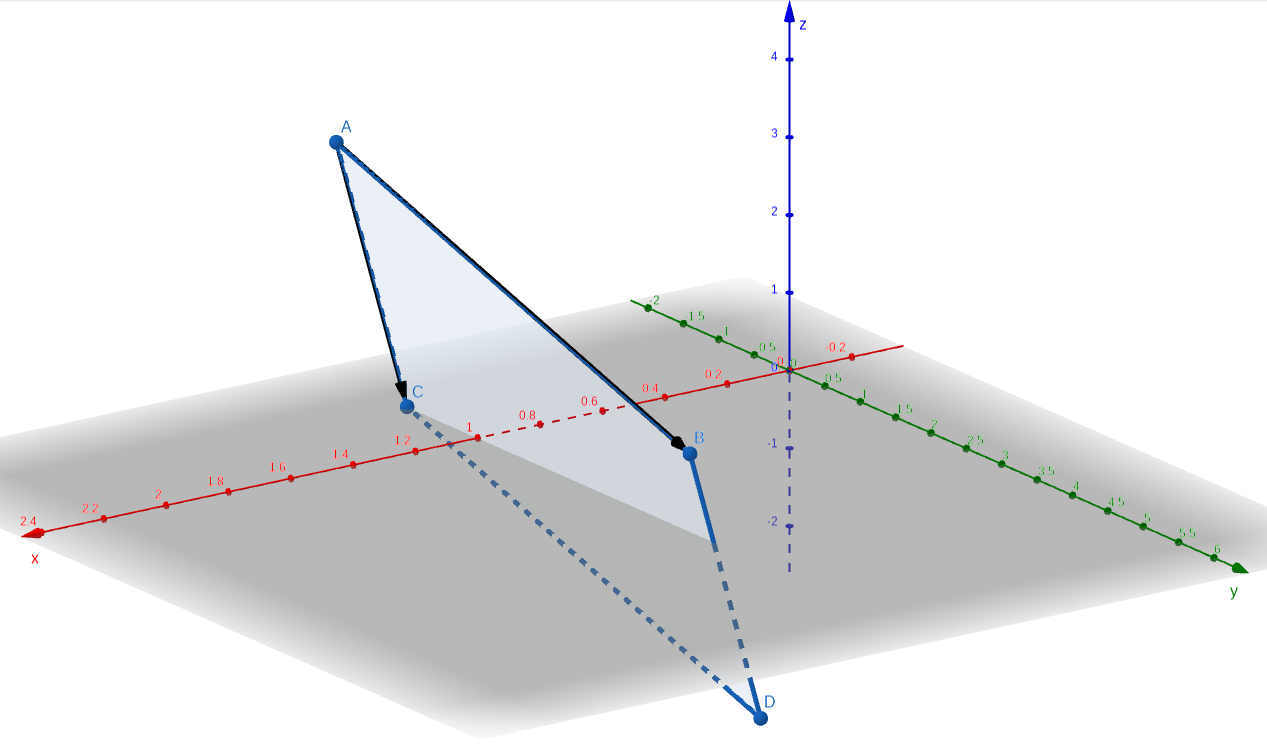
\includegraphics[scale=0.3]{figuras/paralelogramo.png}
\end{center}
	
\end{frame}


\begin{frame}[label=produtovetorial]{}
\begin{casa}
Determine a área do triângulo cujos vértices são os pontos $A=(3,2,0)$, $B=(1,0,2)$ e $C=(0,4,3)$.
\end{casa}
	
\end{frame}





\begin{frame}[label=produtovetorial]{}
\begin{block}{Propriedades do Produto Vetorial}
\begin{enumerate}
	\item $\|\pv{u}{v}\|=0\Leftrightarrow$ $u=0$ ou $v=0$ ou ${u}, {v}$ são múltiplos.
	\item $\pv{u}{v}=-\pv{v}{u}$  (anticomutatividade).
	\item $(\lambda {u})\times {v}={u}\times (\lambda{v})=\lambda(\pv{u}{v})$.
	\item ${u}\times({v}+{w})=\pv{u}{v}+\pv{u}{w}$.
\end{enumerate}
\end{block}
\begin{exe}
Mostre que se $u+v+w=0$, então $u\times v=v\times w$.
\end{exe}
\end{frame}

\subsection*{Distância entre ponto e reta}

\begin{frame}[label=produtovetorial]{Aplicação: Distância de Ponto à reta}
Dados um ponto $A$ e uma reta $\ell$ no espaço. Então, a {\color{blue}distância entre $A$ e $\ell$ } é dada por 
\[{\color{red}d(A,\ell)=\frac{\|AP\times v\|}{\|v\|}},\]
onde $P$ é um ponto e $v$ um vetor diretor  de $\ell$.

\begin{exe}
	Achar a distância entre $A=(3,0,-2)$ e 
	$\ell:\begin{cases}
		x=1-t\\ y=2+2t\\ z=t,\ t\in \R.
	\end{cases}$
\end{exe}
	
\end{frame}


\begin{frame}[label=produtovetorial]{}
\begin{casa}
\begin{enumerate}
	\item Obtenha a reta $r$ dada pela inteseção dos planos $\pi_1: x+y+z=2$ e $\pi_2:x-y-z=0$.
	
	\item Determine os pontos da reta $r$ que estão à distância $\sqrt{6}$ da reta 
$s:\begin{cases}
	x=1+t\\ y=-t\\ z=-1+t,\ t\in \R.
\end{cases}$
\end{enumerate}
\end{casa}
	
\end{frame}

\begin{frame}[label=produtovetorial]{Produto Misto}
\begin{defin}
	O {\color{blue} produto misto} entre os vetores $u,v$ e $w$ em $\R^3$ é o número real
	\[[u,v,w]:=(u\times v)\cdot w.\]
	
Geometricamente $\left| [u,v,w]  \right|$ representa o volume do paralelepípedo cujas arestas são representantes dos vetores $u,v$ e $ w $ com mesma origem.
\end{defin}
	
\end{frame}





\begin{frame}[label=produtovetorial]{}
	
\begin{prop}
	Se $u=(u_1,u_2,u_3)$, $v=(v_1,v_2,v_3)$ e $w=(w_1,w_2,w_3)$, então
\[[u,v,w]=\det
\begin{bmatrix}
	u\\
	v\\
	w
\end{bmatrix}
\]
\end{prop}
\begin{exe}
Determinar o volume do paralelepípedo que tem por arestas adjacentes os segmentos $AB$, $AC$ e $AD$, onde $A=(1,0,1)$, $B=(0,1,1)$, $C=(1,1,1)$ e $D=(1,-1,-1)$.
\end{exe}
\end{frame}

\begin{frame}[label=produtovetorial]{}
\begin{casa}
	Determinar $x$ para que o volume do paralelepípedo que tem um dos vértices no ponto $A=(2,1,6)$ e os três vértices adjacentes nos pontos $B=(4,1,3)$, $C=(1,3,2)$ e $D=(1,x,1)$ seja igual a $15$.
\end{casa}
	
\end{frame}

\begin{frame}[label=produtovetorial]{Distância entre retas}



	
\end{frame}





\section{Subespaços, Base e Dimensão}

\subsection*{Dependência e Independência Linear}

\begin{frame}[label=lild]{Dependência e Independência Linear}
\begin{defin}

Dizemos que um conjunto $S=\{\vec{v}_1,\vec{v}_2,\ldots,\vec{v}_k\}$ de vetores do $\R^n$ é {\color{blue} linearmente independente (LI)} se a equação vetorial
\[x_1\vec{v}_1+x_2\vec{v}_2+\cdots +x_k\vec{v}_k=\vec{0}\]
só possui a solução trivial. Em outras palavras, a única forma de escrever o vetor nulo como combinação linear dos vetores $\vec{v}_1,\vec{v}_2,\ldots, \vec{v}_k$ é aquela em que todos os escalares são iguais a zero. Caso contrário, dizemos que o conjunto $S$ é {\color{blue}linearmente dependente (LD)}.

\end{defin}
	
\end{frame}

\begin{frame}[label=lild]{}
\begin{exe}
Decida se os seguintes conjuntos de vetores são LI ou LD:
\begin{enumerate}
\item $\vec{v}_1=(1,0,1)$, $\vec{v}_2=(0,1,1)$, $\vec{v}_3=(1,1,1)$.

\item  $\vec{v}_1=(1,0,1,2)$, $\vec{v}_2=(2,-1,3,5)$, $\vec{v}_3=(-1,2,-3,-4)$.
\end{enumerate}
\end{exe}

\begin{block}{}
Mostrar que um conjunto $S=\{\vec{v}_1,\vec{v}_2,\ldots,\vec{v}_k\}$ de vetores do $\R^n$ é {\color{red}LI} é equivalente a mostrar que o sistema {\color{red}$AX=0$ tem solução única}, onde $A$ é a matriz cujas {\color{red}colunas são dadas pelos vetores de $S$}.
\end{block}

\begin{exer}
Decida se são LI ou LD os seguintes vetores:
\[
\vec{v}_1=(1,2,-1,-2), \vec{v}_2=(0,1,2,5), \vec{v}_3=(1,0,-4,-1),  \vec{v}_4=(1,-1,2,7).\]
\end{exer}
	
\end{frame}



\begin{frame}[label=lild,fragile=singleslide]{}
\begin{pycode}
import sympy as sp

def pt(Y):
 return((Y[0],Y[1],Y[2]))

v1=sp.Matrix([1,1,2])
v2=sp.Matrix([1,0,1])
v3=sp.Matrix([4,6,12])

A=sp.Matrix.hstack(v1,v2,v3)


u1=sp.Matrix([0,3,1,-1])
u2=sp.Matrix([6,0,5,1])
u3=sp.Matrix([4,-7,1,3])

B=sp.Matrix.hstack(u1,u2,u3)
\end{pycode}
\begin{casa}
Para cada caso, diga se o conjunto de vetores é LI ou LD.

\begin{enumerate}
\item $\{\pyl{pt(v1)},\pyl{pt(v2)}, \pyl{pt(v3)}\}$
\item $\{\pyl{pt(u1)},\pyl{pt(u2)}, \pyl{pt(u3)}\}$
\end{enumerate}
\end{casa}

\end{frame}




\begin{frame}[label=lild]{Propriedades}

\begin{enumerate}
\item Um conjunto formado por um único vetor não nulo é LI.

\item Um conjunto com 2 vetores não nulos é LD se, e somente se, são múltiplos.

\item Um conjunto finito de vetores de $\R^n$ que contém o vetor nulo é LD.

\item Se $\{\vec{v}_1,\vec{v}_2,\ldots,\vec{v}_k\}$ é LD, qualquer conjunto que o contenha também é LD.

\item As colunas de uma matriz $A$ de ordem $n$ são LI se, e somente se, $\det(A)\neq 0$.

\item Em $\R^n$, um conjunto com mais de $n$ vetores é LD.

\item Um conjunto de vetores é LD se, e somente se, {\color{red} pelo menos um dos vetores} pode ser escrito como combinação linear dos demais.
\end{enumerate}


\end{frame}

%---------------------------------------------------------------

\subsection*{Posição Relativa entre retas}

\begin{frame}[label=pos-retas]{Posição relativas entre retas}
	
\only<1,3>{	
\only<1>{No espaço, existem \textcolor{red}{quatro} posições que duas retas $r$ e $s$ podem assumir:
	\bigskip}

\begin{minipage}{0.45\textwidth}
	\begin{center}
		%\textbf{Concorrentes}
		\tdplotsetmaincoords{70}{80}
		\begin{tikzpicture}[tdplot_main_coords]
		
		\node at (0,0,3.5)	{\textbf{Paralelas}};
		
		
		\coordinate (O) at (0, 0, 0);
		
		\filldraw[gray, opacity = 0.5] (-1.5,-2,2) -- (1.5,-2,2) -- (1.5, 2, 2) --(-1.5, 2, 2) -- cycle;
		
		\draw[red,thick]  ($(-1,2,2)-0.2*(2,1,0)$) node[anchor=south] {$s$} -- ($(1,-2,2)-0.2*(2,1,0)$);
	
		\draw[blue,thick] ($(-1,2,2)+0.2*(2,1,0)$) node[anchor=north] {$r$} -- ($(1,-2,2)+0.2*(2,1,0)$);

\only<3>{
\draw plot [mark=*, mark size=1]  coordinates{($(-1,2,2)-0.2*(2,1,0)+0.3*(2,-4,0)$)} node[anchor=south] {{\color{red}$B$}}; 

\draw plot [mark=*, mark size=1] coordinates{($(-1,2,2)+0.2*(2,1,0)+0.7*(2,-4,0)$)} node[anchor=north] {{\color{blue}$A$}}; 

\draw[-{Latex},thick]  ($(-1,2,2)+0.2*(2,1,0)+0.7*(2,-4,0)$) -- ($(-1,2,2)-0.2*(2,1,0)+0.3*(2,-4,0)$);
}
\end{tikzpicture}
\end{center}
\end{minipage}
\begin{minipage}{0.45\textwidth}
	\begin{center}
		\tdplotsetmaincoords{70}{80}
	\begin{tikzpicture}[tdplot_main_coords]
	
	\node at (0,0,3.5)	{\textbf{Coincidentes}};
	
	
	\coordinate (O) at (0, 0, 0);
	
	\filldraw[gray, opacity = 0.5] (-1.5,-2,2) -- (1.5,-2,2) -- (1.5, 2, 2) --(-1.5, 2, 2) -- cycle;
	
	\draw[red,thick] (-1,2,2) node[anchor=south] {$s$} -- (1,-2,2) ;
	
	\draw[blue,thick] ($(-1,2,2)+0.02*(2,1,0)$) node[anchor=north] {$r$} -- ($(1,-2,2)+0.02*(2,1,0)$);
	
	
	\end{tikzpicture}		
	\end{center}
\end{minipage}

\begin{center}
	\tdplotsetmaincoords{70}{80}
\begin{tikzpicture}[tdplot_main_coords]

\draw[red,thick,-latex] ($(0,0,0)$)  -- ($(-1,2,0)$) node[anchor=south] {$\vec{s}$};
\draw[blue,thick,-latex] ($(0,0,0)$) -- ($0.7*(-1,2,0)$) node[anchor=north east] {$\vec{r}$};

\only<3>{\draw[thick,-latex] ($(0,0,0)$) -- ($-0.4*(2,1,0)-0.4*(2,-4,0)$) node[anchor=south east] {$\overrightarrow{{\color{blue}A}{\color{red}B}}$};
}
\end{tikzpicture}	

{\small {\color{blue}$\vec{r}$},{\color{red}$\vec{s}$} são \textcolor{blue}{LD} } 

\end{center}
\only<3>{Se ${\color{blue}\vec{r}}$ e $\overrightarrow{{\color{blue}A}{\color{red}B}}$ são {\color{blue} LI}, então elas são {\color{blue} paralelas}. Caso contrário, são {\color{red} coincidentes}.}
}


\only<2,4>{	
	\begin{minipage}{0.45\textwidth}
		\begin{center}
				\tdplotsetmaincoords{70}{80}
			\begin{tikzpicture}[tdplot_main_coords]
			
			\node at (0,0,3.5)	{\textbf{Concorrentes}};
			
			
			\coordinate (O) at (0, 0, 0);
			

			
			\draw[red,thick] (-1,2,2) node[anchor=south] {$s$} -- (1,-2,2);
			\filldraw[gray, opacity = 0.5] (-1.5,-2,2) -- (1.5,-2,2) -- (1.5, 2, 2) --(-1.5, 2, 2) -- cycle;
			\draw[blue,thick] (-1.5,-1.5,2)  -- (1.5,1.5,2) node[anchor=south] {$r$};

			
		\end{tikzpicture}
		\end{center}
	\end{minipage}
	\begin{minipage}{0.45\textwidth}
	\begin{center}
				\tdplotsetmaincoords{70}{80}
				\begin{tikzpicture}[tdplot_main_coords]
				
				\node at (0,0,3.5)	{\textbf{Reversas}};
				
				
				\coordinate (O) at (0, 0, 0);
				

				\filldraw[gray, opacity = 0.5] (-1.5,-2,0) -- (1.5,-2,0) -- (1.5, 2, 0) --
				(-1.5, 2, 0) -- cycle;				
				\draw[blue,thick] (-1.5,-1.5,0) -- (1.5,1.5,0)node[anchor=south] {$r$};
				
					\draw[red,thick] (-1,2,2) node[anchor=south] {$s$} -- (1,-2,2);
				\filldraw[gray, opacity = 0.5] (-1.5,-2,2) -- (1.5,-2,2) -- (1.5, 2, 2) --(-1.5, 2, 2) -- cycle;
				
				\draw[dashed] (-1.5,-2,0) -- (-1.5,-2,2) ;
		
\only<4>{
\draw plot [mark=*, mark size=1]  coordinates{($(1,-2,2)-0.7*(1,-2,2)+0.7*(-1,2,2)$)} node[anchor=south] {{\color{red}$B$}}; 

\draw plot [mark=*, mark size=1] coordinates{($(-1.5,-1.5,0)+0.3*(1.5,1.5,0)-0.3*(-1.5,-1.5,0)$)} node[anchor=north] {{\color{blue}$A$}}; 

\draw[-{Latex},thick]  ($(-1.5,-1.5,0)+0.3*(1.5,1.5,0)-0.3*(-1.5,-1.5,0)$) -- ($(1,-2,2)-0.7*(1,-2,2)+0.7*(-1,2,2)$);
}		
\end{tikzpicture}
\end{center}
\end{minipage}


\begin{center}
\only<2>{	\tdplotsetmaincoords{70}{80}
	\begin{tikzpicture}[tdplot_main_coords]
	
	\draw[red,thick,-latex] ($(0,0,0)$)  -- ($0.7*(-1,2,0)$) node[anchor=south] {$\vec{s}$};
	\draw[blue,thick,-latex] ($(0,0,0)$) -- ($(1,1,0)$) node[anchor=north east] {$\vec{r}$};
\only<4>{\draw[-{Latex},thick]  (0,0,0) -- ($-1*(-1.5,-1.5,0)-0.3*(1.5,1.5,0)+0.3*(-1.5,-1.5,0)   +(1,-2,2)-0.7*(1,-2,2)+0.7*(-1,2,2)$);}

	\end{tikzpicture}	

{\small {\color{blue}$\vec{r}$},{\color{red}$\vec{s}$} são \textcolor{blue}{LI} } }
\end{center}

\only<4>{
\begin{minipage}{0.6\textwidth}
Se ${\color{blue}\vec{r}}$, ${\color{red}\vec{s}}$ e $\overrightarrow{{\color{blue}A}{\color{red}B}}$ são {\color{blue} LI}, então elas são {\color{blue} reversas}. Caso contrário, são {\color{red} concorrentes}.
\end{minipage}
\begin{minipage}{0.3\textwidth}
	\tdplotsetmaincoords{70}{80}
	\begin{tikzpicture}[tdplot_main_coords]
	
	\draw[red,thick,-latex] ($(0,0,0)$)  -- ($0.7*(-1,2,0)$) node[anchor=south] {$\vec{s}$};
	\draw[blue,thick,-latex] ($(0,0,0)$) -- ($(1,1,0)$) node[anchor=north east] {$\vec{r}$};
\only<4>{\draw[-{Latex},thick]  (0,0,0) -- ($-1*(-1.5,-1.5,0)-0.3*(1.5,1.5,0)+0.3*(-1.5,-1.5,0)   +(1,-2,2)-0.7*(1,-2,2)+0.7*(-1,2,2)$);}

	\end{tikzpicture}	

{\small {\color{blue}$\vec{r}$},{\color{red}$\vec{s}$} são \textcolor{blue}{LI}}
\end{minipage}
}}
\end{frame}


\begin{frame}[label=pos-retas]{Posição relativas entre retas}

\begin{exe}
Estude a posição relativa das retas:
\begin{enumerate}
\item $r: X=(1,2,3)+t(0,1,3)$ e $s: X=(0,1,0)+t(1,1,1)$, $t\in \R.$

\item $r: X=(1,2,3)+t(0,1,3)$ e $s: X=(1,3,6)+t(0,2,6)$, $t\in \R.$

\item $r: X=(1,2,3)+t(0,1,3)$, $t\in \R$ e 
$s: \begin{cases}
x+y+z=6\\
x-y-z=-4
\end{cases}$
\end{enumerate}
\end{exe}

\end{frame}


\subsection*{Subespaço}
\begin{frame}[label=lild]{Subespaço Vetorial}
\begin{defin}
Um subconjunto {\color{red}não-vazio} $V\subset\R^n$ é chamado de {\color{blue} subespaço} de $\R^n$ quando satisfaz:
\begin{enumerate}
\item Se $\vec{u},\vec{v}\in V$, então $\vec{u}+\vec{v}\in V$,
\item Se $\vec{v}\in V$, então $\alpha\vec{v}\in V$, para todo $\alpha\in \R$.
\end{enumerate}
\end{defin}

\begin{exe}
Mostre que o conjunto $V=\{(x,y,z)\in \R^3;z=0\}$ é um subespaço de $\R^3$.
\end{exe}

\end{frame}

\begin{frame}[label=lild]{}
\begin{exe}
\begin{enumerate}
\item Os subespaços vetoriais triviais de $\R^n$ são $V=\{\vec{0}\}$ e o próprio $V=\R^n$.

\item Se $A$ é uma matriz $m\times n$, então o conjunto solução do sistema homogêneo $AX=\vec{0}$ é um subespaço de $\R^n$, chamado de {\color{blue}espaço solução} ou {\color{blue}espaço nulo} ou {\color{blue}núcleo de A} e será denotado por {\color{blue} $\ker(A)$}.

\item Retas e planos em $\R^3$, passando pela origem, são subespaços de $\R^3$.

\item Determine o subespaço de $\R^5$ que é solução do sistema 
\[\left\{
\begin{array}{rrrrrr}
x_1 &+ x_2 & & &+x_5&=0\\
-2x_1 & -2x_2 &+ x_3& -x_4 & -x_5& =0 \\
x_1&+ x_2& -x_3 &+ x_4& &=0
\end{array}\right.
\]
\end{enumerate}
\end{exe}


\end{frame}

\subsection*{Geradores}
\begin{frame}[label=lild]{}
\begin{defin}
Seja $V$ um subespaço de $\R^n$. Dizemos que os vetores $\vec{v}_1,\vec{v}_2,\ldots,\vec{v}_k$, petencentes a $V$, {\color{blue}geram} $V$, se qualquer vetor de $V$ pode ser escrito como combinação linear dos vetores $\vec{v}_1,\vec{v}_2,\ldots,\vec{v}_k$. Neste caso, também dizemos que $V$ é o {\color{blue}subespaço gerado por} $\vec{v}_1,\vec{v}_2,\ldots,\vec{v}_k$ e o denotaremos por $\operatorname{span}\{\vec{v}_1,\vec{v}_2,\ldots,\vec{v}_k\}$.
\end{defin}

\begin{exe}
\begin{enumerate}
\item Determine um conjunto de geradores do núcleo da matriz $A$ do exemplo anterior.

\item Mostre que $\vec{w}=(4,-1,8)$ não está em $\operatorname{span}\{(1,2,-1),(6,4,2)\}$.
\end{enumerate}
\end{exe}
%
%\begin{block}{}
%O espaço solução de um sistema homogêneo $AX=\vec{0}$ é gerado pelas linhas da matriz $A$, também chamado de {\color{blue}espaço linha}.
%\end{block}

\end{frame}

\subsection*{Base}
\begin{frame}[label=lild]{Base}
\begin{defin}
Seja $V$ um subespaço de $\R^n$. Dizemos que um subconjunto $\mathcal{B}=\{\vec{v}_1,\vec{v}_2,\ldots,\vec{v}_k\}$ de $V$ é uma {\color{blue}base} de $V$, se
\begin{enumerate}
\item $\mathcal{B}$ é um conjuntos de geradores de $V$.
\item $\mathcal{B}$ é LI.
\end{enumerate}
\end{defin}
\begin{exe}
\begin{enumerate}
\item O conjunto $\vec{e}_1=(1,0,\ldots,0), \vec{e}_2=(0,1,\ldots,0),\ldots, \vec{e}_n=(0,0,\ldots,1)$ é uma base do $\R^n$, chamada de {\color{blue}base canônica}.
\item Determine uma base para o plano $x+2y-z=0$.
\end{enumerate}

\end{exe}



\end{frame}

\begin{frame}[label=lild]{Dimensão}

\begin{teo}
Se $\mathcal{B}=\{\vec{v}_1,\vec{v}_2,\ldots,\vec{v}_k\}$ é uma base de $V\subset\R^n$, então qualquer outra base tem $k$ elementos. 
\end{teo}


\begin{defin}
A {\color{blue}dimensão} de um subespaço vetorial $V\subset\R^n$ é definido como o número de elementos de uma base de $V$.
\end{defin}

\begin{exe}
 Determine uma base e a dimensão do subespaço $V=\{(a+c,b+c,a+b+2c);\, a,b,c\in \R\}$.

\end{exe}

\end{frame}





\subsection*{Núcleo}
\begin{frame}[label=lild]{Núcleo de uma matriz}
Definimos anteriormente que o {\color{blue}núcleo} de uma matriz $A$ é o espaço solução do sistema $AX=\vec{0}$, denotado por {\color{blue}$\ker(A)$}. {\color{blue}As operações elementares com linhas não alteram o núcleo de uma matriz}. Pode-se mostrar que 
\[{\color{red}\dim(\ker(A))=\operatorname{nulidade}(A)}\]
isto é, o número de variáveis livres do sistema. 
%\[{\color{red} \dim(\ker(A))+\operatorname{posto}(A)=n},\]
%onde $n$ é número de colunas da matriz $A$. 
Vejamos, através do próximo exemplo, um procedimento para obter-se uma base para o núcleo de uma matriz.

\begin{exe}
Determine uma base para o núcleo da matriz
\[
A=\begin{bmatrix}
1 & 3 & -2 & 0 & 2 & 0\\
2 & 6 & -5 & -2& 4& -3& \\
0 & 0& 5& 10& 0 & 15\\
2 & 6& 0&  8& 4& 18
\end{bmatrix}
\]
\end{exe}


\end{frame}

\subsection*{Espaço linha e Espaço coluna}
\begin{frame}[label=lild]{Espaço linha e Espaço coluna}

Dada uma matriz $A$  $m\times n$, além do núcleo de $A$, ainda existem mais dois subespaços associados à ela.
\begin{enumerate}
\item {\color{blue}O espaço linha de $A$}: subespaço de $\R^n$ gerado pela linhas de $A$.
\item {\color{blue}O espaço coluna de $A$}: subespaço de $\R^m$ gerados pelas colunas de $A$.
\end{enumerate}

\begin{teo}
Se uma matriz {\color{red}$R$ está em forma escalonada por linhas}, então os vetores linha não nulos formam uma base do espaço linha de $R$, e os vetores coluna que contém os pivôs formam uma base do espaço coluna. 
\end{teo}

\begin{exampleblock}{}
Em particular, os espaços linha e coluna de $R$ têm a mesma dimensão, apesar de não serem  subespaços de espaços vetoriais diferentes!
\end{exampleblock}

\end{frame}


\begin{frame}[label=lild]{}
Note que a matriz a seguinte matriz está na forma escalonada
\[
R=\begin{bmatrix}
{\color{red}1} & -2 & 5 & 0 & 3\\
0& {\color{red}1}& 3 & 0 & 0 \\
0& 0& 0 & {\color{red}2} & 0\\
0& 0& 0 & 0 & 0
\end{bmatrix}.
\]
Então, 
\begin{itemize}
\item Uma base para o espaço linha de $R$ são os vetores: $\vec{r}_1=(1, -2, 5, 0, 3), \vec{r}_2=(0,1,3,0, 0), \vec{r}_3=(0,0,0,2,0)$ 

\item Uma base para o espaço coluna de $R$ são os vetores:
\[
\vec{c}_1=\begin{bmatrix}
1 \\ 0 \\ 0\\ 0
\end{bmatrix},\
\vec{c}_2=\begin{bmatrix}
-2 \\ 1 \\ 0\\ 0
\end{bmatrix},\
\vec{c}_3=\begin{bmatrix}
0 \\ 0 \\ 2\\ 0
\end{bmatrix}.
\]

\end{itemize}

\end{frame}



\begin{frame}[label=lild]{Obtendo base para os espaço linha}


{\color{blue}As operações elementares com linhas não alteram o espaço linha de uma matriz}, pois as novas linhas são combinações lineares das anteriores e as operações são reversíveis. Portanto, para obter uma base do espaço linha, basta escalonar a matriz.  

\begin{exe}
Determine uma base para o espaço linha da matriz
\[
A=\begin{bmatrix}
1 & -3 & 4 & -2 & 5 & 4\\
2 & -6 & 9 & -1 & 8 & 2\\
2 & -6 & 9 & -1 & 9 & 7\\
-1 & 3& -4 & 2 & -5 & -4
\end{bmatrix}.
\]
\end{exe}
\end{frame}


\begin{frame}[label=lild]{Obtendo base para os espaço coluna}
Diferentemente do espaço linha, as operações elementares com linhas podem alterar o espaço coluna. 

\begin{exe}
As seguintes matrizes são linha-equivalente, mas têm espaços coluna diferentes
\[
A=\begin{bmatrix}
1 & 3\\ 2& 6
\end{bmatrix},\ 
B=\begin{bmatrix}
1 & 3\\ 0 & 0
\end{bmatrix}.
\]
\end{exe}

\end{frame}


\begin{frame}[label=lild]{ }
Dadas duas matrizes ${\color{blue}A}$ e ${\color{red}B}$ linha-equivalentes, sabemos que:
\begin{enumerate}
\item  Os sistemas ${\color{blue}A}X=\vec{0}$ e ${\color{red}B}X=\vec{0}$ {\color{red}têm exatamente as mesmas soluções!}
\item Uma solução $X=\begin{bmatrix}
c_1\\ c_2 \\ \vdots \\ c_n
\end{bmatrix}$ desses sistemas nos dá uma combinação linear das colunas, isto é, se {\color{blue}$A_1, A_2, \ldots, A_n$} e {\color{red}$B_1, B_2,\ldots B_n$} são as respectivas colunas de {\color{blue}$A$} e {\color{red}$B$}, então
\[c_1{\color{blue}A_1}+c_2{\color{blue}A_2}+\cdots c_n{\color{blue}A_n}=\vec{0}\]
\[c_1{\color{red}B_1}+c_2{\color{red}B_2}+\cdots c_n{\color{red}B_n}=\vec{0}\]
\end{enumerate}


Portanto, {\color{blue} as colunas de $A$ são LI se e só se, as colunas de $B$ são LI}. Em outras palavras, {\color{red} ao escalonarmos uma matriz, as colunas mudam mas a dependência linear permanece!}

\end{frame}




\begin{frame}[label=lild]{}

\begin{teo}
Sejam {\color{blue}$A$} e {\color{red}$B$} matrizes linha-equivalentes. 
Um conjunto qualquer de vetores coluna de {\color{blue}$A$} forma uma base do espaço coluna de {\color{blue}$A$} se, e só se, o conjunto de vetores correspondentes de {\color{red}$B$} forma uma base do espaço coluna de {\color{red}$B$}.
\end{teo}

\begin{exe}
Determine uma base para o espaço coluna da matriz
\[
A=\begin{bmatrix}
1 & -3 & 4 & -2 & 5 & 4\\
2 & -6 & 9 & -1 & 8 & 2\\
2 & -6 & 9 & -1 & 9 & 7\\
-1 & 3& -4 & 2 & -5 & -4
\end{bmatrix}.
\]
\end{exe}

\end{frame}

\begin{frame}[label=lild]{Aplicações: obtendo bases de subespaços gerados}
\begin{exe} Considere o subespaço $V$ de $\R^5$ gerado pelos vetores
\[\vec{v}_1=(1,-2,0,0,3), \vec{v}_2=(2,-5,-3,-2,6),
\]
\[\vec{v}_3=(0,5,15,10,0), \vec{v}_4=(2,6,18,8,6).
\]
\begin{enumerate}
\item Determine uma base qualquer de $V$.

\item Determine um subconjunto de $G=\{\vec{v}_1,\vec{v}_2,\vec{v}_3,\vec{v}_4\}$ que forma uma base de $V$.
\item Escreva os vetores de $G$ que não estão na base como combinação linear dos vetores da base.
\end{enumerate}

\end{exe}

\end{frame}


\begin{frame}[label=lild]
\begin{casa} Encontre um subconjunto dos vetores 
\[\vec{v}_1=(1,-2,0,3), \vec{v}_2=(2,-5,-3,6),
\]
\[\vec{v}_3=(0,1,3,0), \vec{v}_4=(2,-1,4,-7), \vec{v}_5=(5,-8,1,2)
\]
que forma uma base para o espaço gerado por eles. Escreva aqueles que não estão na base como uma combinação linear da base. 

\end{casa}
\end{frame}









\subsection*{Coordenadas em relação a uma base de $\R^n$}
\begin{frame}[label=lild]{Coordenadas em relação a uma base}
Se ${\color{red}\mathcal{B}=\{\vec{v}_1,\vec{v}_2,\ldots,\vec{v}_n\}}$ é uma base de $\R^n$, então cada vetor $\vec{v}\in \R^n$ pode ser escrito de forma única como
\[\vec{v}={\color{blue}c_1}{\color{red}\vec{v}_1}+{\color{blue}c_2}{\color{red}\vec{v}_2}+\cdots+{\color{blue}c_n}{\color{red}\vec{v}_n}.\]
Neste caso, dizemos que esta é a {\color{blue}expressão de $\vec{v}$ em termos da base $\mathcal{B}$}. Os escalares {\color{blue}$c_1,c_2,\ldots,c_n$} são chamados de {\color{blue}coordenadas} de $\vec{v}$ em relação à base $\mathcal{B}$ e escrevemos 
\[
[\vec{v}]_{{\color{red}\mathcal{B}}}=
{\color{blue}(c_1,c_2,\ldots,c_n)}_{{\color{red}\mathcal{B}}} \text{ ou }
[\vec{v}]_{{\color{red}\mathcal{B}}}=
{\color{blue}
\begin{bmatrix}
c_1 \\ c_2 \\ \vdots \\ c_n
\end{bmatrix}_{{\color{red}\mathcal{B}}}},
\]
chamado {\color{blue}vetor de coordenadas em relação à base $\mathcal{B}$}.

\end{frame}

\begin{frame}[label=lild]{}
\begin{exe}
\begin{enumerate}
%\item Determine as coordenadas do vetor $\vec{v}=(-1,2,1)$ em relação à base $\mathcal{B}=\{(1,0,1),(0,1,1)\}$ do espaço gerado por $\mathcal{B}$.

\item Determine as coordenadas do vetor $\vec{v}=(2,-1,3)$ em relação à base canônica do $\R^3$, $\mathcal{C}=\{\vec{e}_1,\vec{e}_2,\vec{e}_3\}$.

\item Mostre que $\mathcal{B}=\{(1,2,1),(2,9,0),(3,3,4)\}$ é uma base de $\R^3$. Em seguida, encontre o vetor de coordenadas de $\vec{v}=(5,-1,9)$ em relação a essa base.
\end{enumerate}
\end{exe}
\end{frame}
\section{Autovetores e Autovalores}

\subsection*{Autovetores}

\begin{frame}[label=autovalores]{Autovetores e Autovalores}

\begin{defin}
Seja $A$ uma matriz quadrada de ordem $n$. Dizemos que um vetor {\color{red}não nulo} $\vec{v}\in \R^n$ é um  {\color{blue}autovetor} de $A$ se $A\vec{v}$ for um múltiplo escalar de $\vec{v}$, isto é, se existe  $\lambda \in \R$ tal que 
\[A\vec{v}=\lambda \vec{v}.\]
Neste caso, dizemos que $\lambda$ é um {\color{blue}autovalor} de $A$.

\end{defin}

\begin{exe}
O vetor $\vec{v}=\begin{bmatrix} 1\\2 \end{bmatrix}$ é um autovetor da matriz
$A=\begin{bmatrix}
3 & 0 \\ 8 & -1
\end{bmatrix}
$
\end{exe}

\end{frame}

\begin{frame}[label=autovalores]{}
\begin{teo}
$\lambda\in \R$ é um autovalor de uma matriz $A$ se, e só se, 
\[\det(A-\lambda I)=0.\]
Está equação e dita {\color{blue}equação característica de A}. E o polinômio $p(\lambda)=\det(A-\lambda I)$ é denominado {\color{blue}polinômio característico}.
\end{teo}

\begin{exe}
Determine os autovetores e autovalores da matriz
\[A=
\begin{bmatrix}
1 & -1 \\ -4 & 1
\end{bmatrix}
\]
\end{exe}
\end{frame}


\subsection*{Autoespaço}
\begin{frame}[label=autovalores]{Autoespaço}
Os autovetores associados a um mesmo autovalor $\lambda$ são os vetores não nulos  que satisfazem
\[(A-\lambda I)\vec{x}=\vec{0},\]
isto é, {\color{red}são todos os vetores não nulos} pertencentes ao {\color{red}núcleo de $A-\lambda I$}, chamado de {\color{blue}autoespaço de $A$ associado a $\lambda$} e denotado por $E_{\lambda}$. 


\begin{exe}
Determine uma base dos autoespaços da  matriz 
\[A=\begin{bmatrix}
0 & 0 & -2\\ 1 & 2 & 1 \\ 1 &0& 3
\end{bmatrix}. \]
\end{exe}
\end{frame}

\begin{frame}[label=autovalores,fragile=singleslide]{}
\begin{casa}
\begin{pycode}
import sympy as sp
A=sp.Matrix([[0,0,2,0],[1,0,1,0],[0,1,-2,0],[0,0,0,1]])
\end{pycode}
Considere a matriz
\[A=
\pyl{A}
\]
\begin{enumerate}
\item Determine os autovalores de $A$.
\item  Determine os autoespaços de $A$.
\item  Determine uma base para cada autoespaço e a dimensão.
\end{enumerate}
\end{casa}
\end{frame}


\subsection*{Matrizes Semelhantes}
\begin{frame}[label=autovalores]{Matrizes Semelhantes}
\begin{defin}
Dizemos que uma {\color{red}matriz quadrada} $B$ é {\color{blue}semelhante} a um matriz $A$ quando existir alguma matriz invertível $P$ tal que 
\[B=P^{-1}AP.\]
Neste caso, escrevemos $B\sim A$.
\end{defin}

Matrizes semelhantes têm muitas propriedades em comum, por exemplo, 

\begin{enumerate}
\item Matrizes semelhantes têm o mesmo determinante.
\item Se $A$ e $B$ são semelhantes, então $B^k=P^{-1}A^kP$.
\end{enumerate}


%\begin{center}
%{\color{red}Matrizes semelhantes têm o mesmo determinante.}
%\end{center}



\end{frame}

\begin{frame}[label=autovalores]{}
\begin{exe}
Defina $P$ como a matriz cujas colunas são os autovetores da matriz $A=\begin{bmatrix}
0 & 0 & -2\\ 1 & 2 & 1 \\ 1 &0& 3
\end{bmatrix}$ do exemplo anterior e calcule a matriz  $D=P^{-1}AP$, semelhante a $A$.
\end{exe}

\begin{teo}
Sejam $\lambda_1$ e $\lambda_2$ {\color{red}autovalores distintos} de uma matriz $A$. Se $\mathcal{B}_1$ e $\mathcal{B}_2$ são as bases dos autoespaços $E_{\lambda_1}$ e $E_{\lambda_2}$, respectivamente, então $\mathcal{B}=\mathcal{B}_1\cup \mathcal{B}_2$ é LI.
\end{teo}

\end{frame}


\begin{frame}[label=autovalores]{Diagonalização de Matrizes}
\begin{defin}
Dizemos que uma matriz quadrada $A$ é {\color{blue}diagonalizável} se for semelhante a alguma matriz diagonal, isto é, se existe alguma matriz invertível $P$ tal que $D=P^{-1}AP$ é uma matriz diagonal. Neste caso, dizemos que $P$ {\color{blue}diagonaliza } $A$.
\end{defin}

\begin{teo}
Uma matriz $A$ de ordem $n$ é diagonalizável se, e só se, possui $n$ autovetores linearmente independentes. Neste caso, se $D=P^{-1}AP$ a matriz diagonal $D$ é formada pelos autovalores e a matriz $P$ tem as colunas formadas pelos autovetores.
\end{teo}

\end{frame}

\begin{frame}[label=autovalores,fragile=singleslide]{}
\begin{exe}
\begin{enumerate}
\item Mostre que a seguinte matriz não é diagonalizável
\[
A=\begin{bmatrix}
1& 0 & 0& \\ 1 & 2 & 0\\ -3 & 5 &  2
\end{bmatrix}
\]

\item Calcule $A^n$ onde $A=\begin{bmatrix}
0 & 1 \\ 2 & 1
\end{bmatrix}$

\begin{pycode}
import sympy as sp

A=sp.Matrix([[4,0,1],[2,3,2],[1,0,4]])
\end{pycode}

\item Mostre que a matriz $A$ é diagonalizável e encontre as matrizes diagonal $D$ e a matriz $P$ que diagonaliza $A$.
\[
A=\pyl{A}
\]
\end{enumerate}

\end{exe}

\end{frame}

\begin{frame}[label=autovalores,fragile=singleslide]{}

\begin{casa}
\begin{pycode}
import sympy as sp

A=sp.Matrix([[4,2,2],[2,4,2],[2,2,4]])
B=sp.Matrix([[-1,7,-1],[0,1,0],[0,15,-2]])
\end{pycode}
\begin{enumerate}
\item Mostre que 
\[A=\pyl{A}\]
é diagonalizável e obtenha as matrizes diagonal $D$ e a matriz $P$ que diagonaliza $A$.

\item Calcule $B^{11}$, onde 
\[B=\pyl{B}\]
\end{enumerate}

\end{casa}
\end{frame}

\begin{frame}[label=autovalores,,fragile=singleslide]{Diagonizando com sympy}
	\begin{footnotesize}
\begin{pyverbatim}
import sympy as sp

A=sp.Matrix([[-1, 2, -2, 10],
[0, -7, 6, -30],
[0, 2, 0, 7],
[0, 2, -2, 9]])
[P,D]=A.diagonalize()
display(P)
display(D)
\end{pyverbatim}
	\end{footnotesize}		

\begin{pycode}
import sympy as sp

A=sp.Matrix([[-1, 2, -2, 10], [0, -7, 6, -30], [0, 2, 0, 7], [0, 2, -2, 9]])
[P,D]=A.diagonalize()
\end{pycode}
\[A=\pyl{A},\, P=\pyl{P},\]
\[D=\pyl{D}\]

\end{frame}

\begin{frame}[label=autovalores]{}


\end{frame}

\section{Ortogonalidade}

\subsection*{Vetores Ortogonais}

\begin{frame}[label=orto]{Vetores Ortogonais}
\begin{exer}
Considere os vetores $\vec{v}_1=(2,1,-1)$, $\vec{v}_2=(1,0,2)$ e $\vec{v}_3=(2,-5,-1)$. 

\begin{enumerate}
\item Mostre que os três vetores são ortogonais dois a dois.

\item Use esse fato para mostrar que os vetores são LI, isto é, a equação vetorial 
\[x\vec{v}_1+y\vec{v}_2+z\vec{v}_3=\vec{0},\]
{\color{red}só possui} a solução trivial $x=y=z=0$.

\item Escreva  $\vec{v}=(3,-1,1)$ como combinação linear da base $\mathcal{B}=\{\vec{v}_1,\vec{v}_2,\vec{v}_3\}$.
\end{enumerate}
\end{exer}

\end{frame}

\begin{frame}[label=orto]{}
\begin{defin}
Um conjunto de vetores $\{\vec{v}_1,\vec{v}_2,\ldots, \vec{v_k}\}\subset \R^n$ é dito {\color{blue}ortogonal} se todos os vetores são ortogonais dois a dois, isto é,
\[\vec{v}_i\cdot \vec{v}_j=0,\ \forall i,j=1,2,\ldots k, \ i\neq j.\]
E dizemos que {\color{blue}ortonormal} se além de ortogonal cada vetor for unitário, isto é, 
\[\|\vec{v}_i\|=1,\ \forall i=1,2,\ldots,k.\]
Neste caso, escrevemos também
\[
\vec{v}_i\cdot \vec{v}_j=\delta_{ij}=
\begin{cases}
1, & i=j\\ 0, & i\neq j
\end{cases}, \ \forall i,j=1,2,\ldots,k
\]
onde $\delta_{ij}$ é o chamado {\color{blue}Delta de Kronecker}.
\end{defin}

\end{frame}

\begin{frame}[label=orto]{}
\begin{teo}
Se $\{\vec{v}_1,\vec{v}_2,\ldots, \vec{v}_k\}$  de $\R^n$  é ortogonal, então esses vetores são LI. Além disso, se
\[\vec{v}=c_1\vec{v}_1+c_2\vec{v}_2+\cdot +c_k\vec{v}_k,\]
então
\[c_i=\frac{\vec{v}\cdot \vec{v}_i}{\|\vec{v}_i\|^2}\] 
\end{teo}

\begin{defin}
Definimos a {\color{blue}projeção ortogonal} de um $\vec{v}$ sobre um vetor  {\color{red} não nulo} $\vec{w}$ como sendo o seguinte vetor
\[\proj_{\vec{w}}\vec{v}=\left(\frac{\vec{v}\cdot \vec{w}}{\|\vec{w}\|^2}\right)\vec{w}.\]
\end{defin}


\end{frame}

%\begin{frame}[label=orto]{Processo de Ortogonalização de Gram-Schimidt}
%\begin{prop}
%Seja $\{\vec{v}_1,\vec{v}_2,\ldots, \vec{v}_k\}$ um conjunto ortogonal  de $\R^n$. Então, para qualquer $\vec{v}\in \R^n$, temos que
%\[\vec{v}-\proj_{{\vec{v}_1}}\vec{v}-\proj_{{\vec{v}_2}}\vec{v}-\cdots-\proj_{{\vec{v}_k}}\vec{v}\]
%é ortogonal a cada $\vec{v}_i$, onde $i=1,2,\ldots,k$.
%\end{prop}
%
%\begin{exe}
%Determine uma base ortogonal para o subespaço de $\R^5$ gerado por
%\[\vec{v}_1=(-1,0,-1,0,1),\ \vec{v}_2=(0,0,1,1,0),\ \vec{v}_3=(-1,1,0,0,0).\]
%\end{exe}
%\end{frame}


\subsection*{Processo de ortonalização de Gram-Schmidt}
%\begin{frame}[label=orto]{Processo de ortonalização de Gram-Schmidt}
%\begin{prop}
%Seja $\{\vec{w}_1,\vec{w}_2,\ldots, \vec{w}_k\}$ um {\color{blue}conjunto 
%ortogonal}  de $\R^n$. Então, para qualquer ${\color{red}\vec{v}}\in \R^n$,
% temos que
%\[\vec{w}={\color{red}\vec{v}}-\proj_{{\vec{w}_1}}{\color{red}\vec{v}}
%-\proj_{{\vec{w}_2}}{\color{red}\vec{v}}-\cdots-\
%\proj_{{\vec{w}_k}}{\color{red}\vec{v}}\]
%é ortogonal a cada $\vec{w}_i$, onde $i=1,2,\ldots,k$. Além disso, $\vec{w}$ 
%está no mesmo espaço gerado por $\{\vec{w}_1,\vec{w}_2,\ldots, \vec{w}_k,{\color{red}\vec{v}}\}$.
%\end{prop}
%
%
%\begin{exe}
%Sejam $W$ o subespaço gerado por $\vec{v}_1=(1,-1,-1,1)$ e $\vec{v}_2=(2,1,0,1)$. Obtenha uma base ortogonal para $W$.
%\end{exe}
%\end{frame}


\begin{frame}[label=orto]{Processo de ortonalização de Gram-Schmidt}
Seja $\{v_1,v_2,\ldots, v_k \}$ uma base para um subespaço $W$ de $\R^n$. 
Podemos obter uma base ortogonal para $W$ através do seguinte processo, conhecido como {\color{blue}Processo de Ortogonalização de Gram-Schmidt}.
\begin{align*}
& \vec{w}_1=\vec{v}_1,\\
& \vec{w}_2=\vec{v}_2-\proj_{{\vec{w}_1}}\vec{v}_2,\\
& \vec{w}_3=\vec{v}_3-\proj_{{\vec{w}_1}}\vec{v}_3
-\proj_{{\vec{w}_2}}\vec{v}_3,\\
& \vdots\\
& \vec{w}_k=\vec{v}_k-\proj_{{\vec{w}_1}}\vec{v}_k
-\proj_{{\vec{w}_2}}\vec{v}_k-\cdots-\proj_{{\vec{w}_{k-1}}}\vec{v}_k
\end{align*}


\begin{exe}
Determine uma base ortogonal para o subespaço de $\R^5$ gerado por
\[\vec{v}_1=(-1,0,-1,0,1),\ \vec{v}_2=(0,0,1,1,0),\ \vec{v}_3=(-1,1,0,0,0).\]
\end{exe}

\end{frame}




\begin{frame}[label=orto]{}

\begin{casa}
Determine uma base ortogonal para o subespaço de $\R^4$ gerado por
\[\vec{v}_1=(1,-1,-1,1),\ \vec{v}_2=(2,1,0,1),\ \vec{v}_3=(2,2,1,2).\]
\end{casa}
\end{frame}



\section{Diagonalilzação de Matrizes Simétricas}


\subsection*{Matrizes Ortogonais}
\begin{frame}[label=orto]{Matrizes Ortogonais}

\begin{defin}
Uma matriz quadrada $Q$ cujas colunas formam um conjunto ortonormal é chamada 
de \dt{matriz ortogonal}.
\end{defin}

\begin{teo}
Seja $Q$ uma matriz $m\times n$. Suas colunas formam um conjunto ortogonal se, 
e somente se, $Q^TQ=I_n$. Em particular, $Q$ é ortogonal se, e somente se, $Q^{-1}=Q^T$.
\end{teo}

\begin{exe}
Mostre que  a seguinte matriz de rotação é ortogonal.
\[R_\theta= 
\begin{bmatrix}
\cos(\theta) & -\sen(\theta)\\
\sen(\theta) & \cos(\theta)
\end{bmatrix}
\]
\end{exe}

\end{frame}


\begin{frame}[label=orto]{}

\begin{exe}
Mostre que  a seguinte matriz é diagonalizável
\[A=
\begin{bmatrix}
1& 2\\ 2 & -2
\end{bmatrix}.
\]
Em seguida, obtenha $Q$ ortogonal que diagonalize $A$.
\end{exe}

\begin{defin}
Uma matriz quadrada $A$ é \dt{ortogonalmente diagonalizável} se é 
diagonalizável e a matriz $Q$ que a diagonaliza é ortogonal.
\end{defin}

\begin{prop}
Se $A$ é uma matriz simétrica, então os autovetores associados a autovalores distintos são ortogonais.
\end{prop}

\end{frame}

\subsection*{Teorema Espectral}

\begin{frame}[label=orto]{}

\begin{block}{Teorema Espectral}
Uma matriz  $A$ quadrada com entradas reais  é ortogonalmente diagonalizável se, e somente se, $A$ é simétrica.
\end{block}

\begin{exe}
Encontre  uma diagonalização ortogonal para a matriz
\[A=
\begin{bmatrix}
1 & 2 & 1\\ 1& 2 & 1 \\ 1 & 1 & 2
\end{bmatrix}
\]
\end{exe}

\end{frame}



\subsection*{Coordenadas em relação a uma base de $\R^n$}
\begin{frame}[label=lild]{Coordenadas em relação a uma base}
Se ${\color{red}\mathcal{B}=\{\vec{v}_1,\vec{v}_2,\ldots,\vec{v}_n\}}$ é uma base de $\R^n$, então cada vetor $\vec{v}\in \R^n$ pode ser escrito de forma única como
\[\vec{v}={\color{blue}c_1}{\color{red}\vec{v}_1}+{\color{blue}c_2}{\color{red}\vec{v}_2}+\cdots+{\color{blue}c_n}{\color{red}\vec{v}_n}.\]
Neste caso, dizemos que esta é a {\color{blue}expressão de $\vec{v}$ em termos da base $\mathcal{B}$}. Os escalares {\color{blue}$c_1,c_2,\ldots,c_n$} são chamados de {\color{blue}coordenadas} de $\vec{v}$ em relação à base $\mathcal{B}$ e escrevemos 
\[
[\vec{v}]_{{\color{red}\mathcal{B}}}=
{\color{blue}(c_1,c_2,\ldots,c_n)}_{{\color{red}\mathcal{B}}} \text{ ou }
[\vec{v}]_{{\color{red}\mathcal{B}}}=
{\color{blue}
\begin{bmatrix}
c_1 \\ c_2 \\ \vdots \\ c_n
\end{bmatrix}_{{\color{red}\mathcal{B}}}},
\]
chamado {\color{blue}vetor de coordenadas em relação à base $\mathcal{B}$}.

\end{frame}

\begin{frame}[label=lild]{}
\begin{exe}
\begin{enumerate}
%\item Determine as coordenadas do vetor $\vec{v}=(-1,2,1)$ em relação à base $\mathcal{B}=\{(1,0,1),(0,1,1)\}$ do espaço gerado por $\mathcal{B}$.

\item Determine as coordenadas do vetor $\vec{v}=(2,-1,3)$ em relação à base canônica do $\R^3$, $\mathcal{C}=\{\vec{e}_1,\vec{e}_2,\vec{e}_3\}$.

\item Mostre que $\mathcal{B}=\{(1,2,1),(2,9,0),(3,3,4)\}$ é uma base de $\R^3$. Em seguida, encontre o vetor de coordenadas de $\vec{v}=(5,-1,9)$ em relação a essa base.
\end{enumerate}
\end{exe}
\end{frame}
%\section{Cônicas}


\subsection*{Completamento de Quadrados}


\begin{frame}[label=comp]
	\frametitle{Completamento de Quadrados}
	%\begin{scriptsize}
	
\begin{block}{Produto Notáveis}
	\[(x+k)^2=x^2+2k\cdot x+k^2\]
	\[(x-k)^2=x^2-2k\cdot x+k^2\]
\end{block}	

\begin{exe}
	Resolva as seguintes equações sem usar a fórmula de Bhaskara
	\begin{multicols}{2}
		\begin{enumerate}
			\item $x^2-x=0$
			\item $4x^2-1=0$
			\item $x^2-2x=8$
			\item $x^2-8x=9$
		\end{enumerate}
	\end{multicols}
	\medskip
\end{exe}

\end{frame}


\begin{frame}[label=comp]
	\begin{exe}
Complete os quadrados:
\begin{enumerate}
	\item $x^2+7x$
	\item $-2x^2+8x$
\end{enumerate}
	\end{exe}

\begin{block}{Fórmula de Bhaskara}
	Sejam  $a,b$ e $c\in\R$ com $a\neq 0$. Então as soluções da equação $ax^2+bx+c=0$ são dadas por
	\[ x=\frac{-b\pm \sqrt{b^2-4ac}}{2a}\]
\end{block}
\end{frame}

\begin{frame}[label=comp]
	
\begin{casa}
	Complete os quadrados:
\begin{enumerate}
	\item $x^2-4x$
	\item $-x^2+2x$
	\item $3x^2-9x$
\end{enumerate}
\end{casa}

\end{frame}

\subsection*{Elipse}

\begin{frame}[label=conicas]
	\frametitle{Elipse}
	%\begin{scriptsize}
	\uncover<1->{\begin{defin}[Elipse]
			Dados dois pontos no plano $F_1$ e $F_2$ uma \dest{elipse} é o lugar geométrico dos pontos do plano cuja soma das distâncias aos pontos $F_1$ e $F_2$ é constante. Os pontos $F_1$ e $F_2$ são chamados \dest{focos} da elipse.
		\end{defin}
	}

\begin{center}
	\begin{tikzpicture}
   \draw[thick,red] (0,0) ellipse (2cm and 1cm);
   \draw[fill,blue] (1.7,0) circle (1.5pt);
   \draw[fill,blue] (-1.7,0) circle (1.5pt);   
   \node[below left,blue] at (1.7,0) {$F_2$};
   \node[below right,blue] at (-1.7,0) {$F_1$};
   \node[above,red] at (1.2,0.8) {$P$};
 
   \draw (-1.7,0) -- (1.2,0.8) --(1.7,0);
     \draw[fill,red] (1.2,0.8) circle (1.5pt);
\end{tikzpicture}
\end{center}
\end{frame}


\begin{frame}[label=conicas]{Notação}
\begin{minipage}{0.4\textwidth}
	\begin{itemize}
	\item<1-> $F_1, F_2$: focos
		\item<2-> $F_1F_2$: segmento focal
		\item<3-> $O$: centro da elipse
		\item<5-> $A_1,A_2,B_1,B_2:$ Vértices
		
		\item<6-> $A_1A_2$: Eixo maior
		
		\item<7-> $B_1B_2$: Eixo menor
		
		\item<8-> $d(F_1,F_2)$: amplitude focal
	\end{itemize}
\end{minipage}
\begin{minipage}{0.4\textwidth}
	\begin{center}
		\begin{tikzpicture}
\uncover<2->{		\draw (-2.5,0) -- (2.5,0);
				\draw[thick,blue] (-1.3,0)--(1.3,0);  }
\uncover<4->{	\draw (0,-1.5) -- (0,1.5);}
%		\node[below right] at (2.5,0) {$x$};
%		\node[above left] at (0,1.5) {$y$};		
\uncover<1->{	\draw[thick,red] (0,0) ellipse (2cm and 1cm);}
\uncover<1->{		\draw[fill,blue] (1.3,0) circle (1.5pt);
		\draw[fill,blue] (-1.3,0) circle (1.5pt);   
	\node[below] at (1.3,0) {$F_2$};
		%	\node[below right,blue] at (-1.7,0) {$F_1$};
		\node[below] at (-1.3,0) {$F_1$};}
\uncover<5->{\draw[fill,red] (2,0) circle (1.5pt);   	
		\draw[fill,red] (-2,0) circle (1.5pt);
		\draw[fill,red] (0,1) circle (1.5pt);   	
		\draw[fill,red] (0,-1) circle (1.5pt);
		\node[above right] at (2,0) {$A_2$};
		\node[above left] at (-2,0) {$A_1$};
		\node[left] at (0,1.2) {$B_2$};
		\node[left] at (0,-1.2) {$B_1$};}
\uncover<3->{		\node[below left] at (0,0) {$O$};
		\draw[fill] (0,0) circle (1.5pt);}
		%	\draw (0,1) -- (1.3,0);
\uncover<6->{\draw[decoration={brace,mirror,raise=5pt},decorate] (-2,-1.6)--(2,-1.6);
			\draw[dashed] (-2,0) -- (-2,-1.6);
		\draw[dashed] (2,0) -- (2,-1.6); 
	\node[below] at (0,-1.8) {eixo maior};}	
\uncover<7->{\draw[decoration={brace,mirror,raise=5pt},decorate] (2.5,-1)--(2.5,1);
	\draw[dashed] (0,-1) -- (2.5,-1);
	\draw[dashed] (0,1) -- (2.5,1);
	\node[text width=1.cm] at (3.5,0) {eixo  menor};}

\uncover<8->{\draw[decoration={brace,raise=5pt},decorate] (-1.3,1.6)--(1.3,1.6);
\draw[dashed] (-1.3,0) -- (-1.3,1.6);
\draw[dashed] (1.3,0) -- (1.3,1.6); 
\node[below] at (0,2.4) {amplitude focal};}		

	
		
		%	\node at (-5,2) {$A_1,A_2,B_1,B_2:$ Vétices};
		
		%\node[above,red] at (1.2,0.8) {$P$};
		
		%\draw (-1.7,0) -- (1.2,0.8) --(1.7,0);
		%\draw[fill,red] (1.2,0.8) circle (1.5pt);
		\end{tikzpicture}
	\end{center}
\end{minipage}

	%\end{scriptsize}
\end{frame}


\begin{frame}[label=conicas]
	\uncover<1->{\begin{block}{}
			Dado uma elipse, considere um sistema de eixos cartesianos com eixo $OX$ determinado segmento focal, com origem no centro da elipse. Neste caso, sendo $2c$ a amplitude focal,  $2a$  a soma das distâncias de um ponto qualquer da elipse aos focos e $b^2=a^2-c^2$, então a equação da elipse é dada por
			
			\begin{center}
				\textcolor{red}{\fbox{$\displaystyle\frac{x^2}{a^2}+\frac{y^2}{b^2}=1$}}
			\end{center}
		A razão $e=\frac{c}{a}$ é chamada \dest{excentricidade da elipse} e, no caso, mede o achatamento da elipse. 
	\end{block}}


	\begin{center}
	\begin{tikzpicture}
	\draw[->] (-2.5,0) -- (2.5,0);
	\draw[->] (0,-1.5) -- (0,1.5);
	\node[below right] at (2.5,0) {$x$};
	\node[above left] at (0,1.5) {$y$};		
	\draw[thick,red] (0,0) ellipse (2cm and 1cm);
	\draw[fill,blue] (1.3,0) circle (1.5pt);
	\draw[fill,blue] (-1.3,0) circle (1.5pt);   
	\node[below] at (1.3,0) {$c$};
	%	\node[below right,blue] at (-1.7,0) {$F_1$};
	\node[below] at (-1.5,0) {$-c$};
	\draw[fill,red] (2,0) circle (1.5pt);   	
	\draw[fill,red] (-2,0) circle (1.5pt);
	\draw[fill,red] (0,1) circle (1.5pt);   	
	\draw[fill,red] (0,-1) circle (1.5pt);
	\node[below right] at (2,0) {$a$};
	\node[below left] at (-2,0) {$-a$};
	\node[left] at (0,1.2) {$b$};
	\node[left] at (0,-1.2) {$-b$};
	\draw (0,1) -- (1.3,0);
	\node at (0.8,0.7) {$a$};
	\node at (3,1) {$a^2=b^2+c^2$};
	\end{tikzpicture}
\end{center}

	
	%\end{scriptsize}
\end{frame}




\begin{frame}[label=conicas]
	\begin{obs}
		Note que como posicionamos os focos no eixo $OX$, temos que $b<a$. No caso em que os focos estiverem sobre o eixo $OY$, a equação terá a mesma forma, entretanto com $b>a$ e satisfazendo $a^2=b^2-c^2$.
	\end{obs}
	
	
\begin{center}
	\begin{tikzpicture}
	\draw[->] (0,-2.5) -- (0,2.5);
	\draw[->] (-1.5,0) -- (1.5,0);
	\node[below right] at (1.5,0) {$x$};
	\node[above left] at (0,2.5) {$y$};		
	\draw[thick,red] (0,0) ellipse (1cm and 2cm);
	\draw[fill,blue] (0,1.3) circle (1.5pt);
	\draw[fill,blue] (0,-1.3) circle (1.5pt);   
	\node[left] at (0,1.3) {$c$};
	%	\node[below right,blue] at (-1.7,0) {$F_1$};
	\node[left] at (0,-1.3) {$-c$};
	\draw[fill,red] (0,2) circle (1.5pt);   	
	\draw[fill,red] (0,-2) circle (1.5pt);
	\draw[fill,red] (1,0) circle (1.5pt);   	
	\draw[fill,red] (-1,0) circle (1.5pt);
	\node[left] at (0,2.2) {$b$};
	\node[left] at (0,-2.2) {$-b$};
	\node[below] at (1.2,0) {$a$};
	\node[below] at (-1.3,0) {$-a$};
	\draw (1,0) -- (0,1.3);
	\node at (0.7,0.8) {$b$};
	\node at (3,1) {$b^2=a^2+c^2$};
	\node[red] at (-3,1) {$\displaystyle\frac{x^2}{a^2}+\frac{y^2}{b^2}=1$};
	
	%\node[above,red] at (1.2,0.8) {$P$};
	
	%\draw (-1.7,0) -- (1.2,0.8) --(1.7,0);
	%\draw[fill,red] (1.2,0.8) circle (1.5pt);
	\end{tikzpicture}
\end{center}

	
\end{frame}

\begin{frame}[label=conicas]
		\begin{exe}
		Encontre as coordenadas dos focos e faça um esboço das seguintes elipses.
		\begin{enumerate}
			\item  $4x^2+9y^2=36$ 
			\item  $5x^2+2y^2=15$ 
		\end{enumerate}
		
	\end{exe}

\begin{exe}
	Escreva uma equação da elipse cujos focos são $(0,6)$ e $(0,-6)$ e o eixo maior mede 20.
\end{exe}
\end{frame}

\begin{frame}[label=conicas]
	\begin{casa}
		\begin{enumerate}
			\item Encontre os focos e faça um esboço da  elipse $x^2+2y^2=4$.
			
			\item Determine a equação da elipse cujos focos estão sobre o eixo $OY$, o eixo maior mede 10 e a amplitude focal é 6.
			
			
			\item Prove que o ponto $P=(2\sen t,\cos t)$ pertence a uma elipse, qualquer que seja o valor de $t\in \R$.
			
				\item Assistir ao filme \textit{Alexandria}\footnotemark\ (título original: Ágora). Direção: Alejandro Amenábar.
			\footnotetext{\href{https://www.imdb.com/title/tt1186830/}{Alexandria (2009) - IMDb - https://www.imdb.com/title/tt1186830/}}
		\end{enumerate}
	\end{casa}
	
	
\end{frame}


%%%%%%%%%%%%%%%%%%%%%%%%%%%%%%%%%%%%%%%%%%%%%%%%%%%%%%%%%%%

\subsection*{Hipérbole}

\begin{frame}[label=conicas]{Hipérbole}
	%\begin{scriptsize}
	\uncover<1->{\begin{defin}[Hipérbole]
			Dados dois pontos no plano $F_1$ e $F_2$ uma \dest{hipérbole} é o lugar geométrico dos pontos do plano cujo valor absoluto da diferença das distâncias aos pontos $F_1$ e $F_2$ é uma constante positiva menor que a distância entre os pontos $F_1$ e $F_2$. Os pontos $F_1$ e $F_2$ são chamados \dest{focos} da hipérbole.
		\end{defin}
	}
	
	\begin{center}
%		%	\pgfmathsetmacro{\a}{1}
%		\pgfmathsetmacro{\b}{2}	
		\begin{tikzpicture}	
		\def\a{1.5}	
		\def\b{1}			
		 \draw[scale=0.5,domain=-1.5:1.5,smooth,variable=\t,red,thick]
		  plot ({\a*cosh(\t )},{\b*sinh(\t)});
		   \draw[scale=0.5,domain=-1.5:1.5,smooth,variable=\t,red,thick]
		  plot ({-\a*cosh(\t )},{\b*sinh(\t)});
		\draw[fill,blue] (1.8,0) circle (1.5pt);
		\draw[fill,blue] (-1.8,0) circle (1.5pt);   
		\node[below,blue] at (1.8,0) {$F_2$};
		\node[below,blue] at (-1.8,0) {$F_1$};
		\node[above,red] at (1.2,0.8) {$P$};
%		
		\draw (-1.8,0) -- (1.4,0.8) --(1.8,0);
		\draw[fill,red] (1.4,0.8) circle (1.5pt);
		\end{tikzpicture}
	\end{center}
	
\end{frame}


\begin{frame}[label=conicas]{Notação}
	\begin{minipage}{0.4\textwidth}
		\begin{itemize}
			\item<1-> $F_1, F_2$: focos
			\item<2-> $F_1F_2$: segmento focal
			\item<3-> eixo focal
			\item<4-> $O$: centro da Hipérbole
			\item<5-> $A_1,A_2:$ Vértices
			\item<6-> $d(F_1,F_2)$: amplitude ou distância focal
		\end{itemize}
	\end{minipage}
	\begin{minipage}{0.5\textwidth}
		\begin{center}
			\begin{tikzpicture}
				\def\a{1.5}	
			\def\b{1}			
		
		
			%		
%			\draw (-1.8,0) -- (1.4,0.8) --(1.8,0);
%			\draw[fill,red] (1.4,0.8) circle (1.5pt);
	\uncover<1->{	\draw[scale=1,domain=-1.5:1.5,smooth,variable=\t,red,thick]
	plot ({\a*cosh(\t )},{\b*sinh(\t)});
	\draw[scale=1,domain=-1.5:1.5,smooth,variable=\t,red,thick]
	plot ({-\a*cosh(\t )},{\b*sinh(\t)});
	\draw[fill,blue] (1.8,0) circle (1.5pt);
	\draw[fill,blue] (-1.8,0) circle (1.5pt);   
	\node[below,blue] at (1.8,0) {$F_2$};
	\node[below,blue] at (-1.8,0) {$F_1$};
}
					\uncover<3->{	\draw (-3.5,0) -- (3.5,0);
					}	
			\uncover<2->{	
				\draw[thick,blue] (-1.8,0)--(1.8,0);  }
						
			\uncover<4->{	\node[below left] at (0,0) {$O$};
				\draw[fill] (0,0) circle (1.5pt);}
		%	\uncover<5->{	\draw (0,-1.5) -- (0,1.5);}
			%		\node[below right] at (2.5,0) {$x$};
			%		\node[above left] at (0,1.5) {$y$};		
		
			\uncover<5->{\draw[fill,red] (\a,0) circle (1.5pt);   	
				\draw[fill,red] (-\a,0) circle (1.5pt);
%				\draw[fill,red] (0,1) circle (1.5pt);   	
%				\draw[fill,red] (0,-1) circle (1.5pt);
				\node[above left,red] at (\a,0) {$A_2$};
				\node[above right,red] at (-\a,0) {$A_1$};
%				\node[left] at (0,1.2) {$B_2$};
%				\node[left] at (0,-1.2) {$B_1$};
}
		
			%	\draw (0,1) -- (1.3,0);
			\uncover<6->{\draw[decoration={brace,mirror,raise=5pt},decorate] (-1.8,-1.6)--(1.8,-1.6);
				\draw[dashed] (-1.8,0) -- (-1.8,-1.6);
				\draw[dashed] (1.8,0) -- (1.8,-1.6); 
				\node[below] at (0,-1.8) {amplitude focal};}	
%			\uncover<7->{\draw[decoration={brace,mirror,raise=5pt},decorate] (2.5,-1)--(2.5,1);
%				\draw[dashed] (0,-1) -- (2.5,-1);
%				\draw[dashed] (0,1) -- (2.5,1);
%				\node at (4,0) {eixo menor};}	
			
			
			
			%	\node at (-5,2) {$A_1,A_2,B_1,B_2:$ Vétices};
			
			%\node[above,red] at (1.2,0.8) {$P$};
			
			%\draw (-1.7,0) -- (1.2,0.8) --(1.7,0);
			%\draw[fill,red] (1.2,0.8) circle (1.5pt);
			\end{tikzpicture}
		\end{center}
	\end{minipage}
	
	%\end{scriptsize}
\end{frame}



\begin{frame}[label=conicas]
		\uncover<1->{\begin{block}{}
			Dado uma hipérbole, considere um sistema de eixos cartesianos tomando-se  $OX$ como o eixo focal e a origem como o centro da hipérbole. Neste caso, sendo $2c$ a distância focal,  $2a$ o valor absoluto da diferença das distâncias de um ponto qualquer da hipérbole aos focos, onde $0<a<c$ e $c^2=b^2+a^2$, então a equação da hipérbole é dada por
			
			\begin{center}
				\textcolor{red}{\fbox{$\displaystyle\frac{x^2}{a^2}-\frac{y^2}{b^2}=1$}}
			\end{center}
	\end{block}}

	\begin{center}
	%		%	\pgfmathsetmacro{\a}{1}
	%		\pgfmathsetmacro{\b}{2}	
	\begin{tikzpicture}	
	\def\a{1.5}	
	\def\b{1}			
	
	
	\coordinate (AB) at (\a,\b);
	\coordinate (ABm) at (-\a,-\b);
	\coordinate (mAB) at (-\a,\b);
		\coordinate (AmB) at (\a,-\b);
	
	
	\draw[domain=-1.5:1.5,smooth,variable=\t,red,thick]
	plot ({\a*cosh(\t )},{\b*sinh(\t)});
	\draw[domain=-1.5:1.5,smooth,variable=\t,red,thick]
	plot ({-\a*cosh(\t )},{\b*sinh(\t)});
	\draw[fill,blue] (1.8,0) circle (1.5pt);
	\draw[fill,blue] (-1.8,0) circle (1.5pt);   
	\node[below,blue] at (1.8,0) {$c$};
	\node[below left,blue] at (-1.8,0) {$-c$};
		
	
	
	\uncover<1->{	\draw[->] (-3.5,0) -- (3.5,0);
}	
\draw[blue,thick] (0,\b) -- (\a,0);
\node[blue] at (0.7,0.7) {$c$};
	\uncover<1->{	\draw[->] (0,-2.) -- (0,2);}
		\node[below right] at (3.5,0) {$x$};
		\node[above left] at (0,2) {$y$};
		
		
		
		\draw [shorten >= -2.5cm, shorten <=-2.5cm,dashed] (AB)--(ABm);
		\draw [shorten >= -2.5cm, shorten <=-2.5cm,dashed] (mAB)--(AmB);
		\draw[dashed] (AB) -- (AmB) -- (ABm) -- (mAB) -- (AB);
		
		
			\draw[fill,red] (\a,0) node[below left] {$a$} circle (1.5pt);
		\draw[fill,red] (-\a,0) node[below right] {$-a$} circle (1.5pt);
		
			\draw[fill] (0,\b) node[above left] {$b$} circle (1.5pt);
		\draw[fill] (0,-\b) node[below left] {$-b$} circle (1.5pt);
			
\node[blue] at (5,1) {$c^2=a^2+b^2$};



	\end{tikzpicture}
\end{center}
\end{frame}



\begin{frame}[label=conicas]
	\begin{minipage}{0.5\textwidth}
		\begin{obs}
 No caso em que os focos estiverem sobre o eixo $y$, a equação terá uma forma semelhante, com o sinal de menos acompanhando o termo com $x$ e consequentemente interceptará o eixo $y$ em $y=b$ e $y=-b$
	\end{obs}
	\end{minipage}
	\begin{minipage}{0.4\textwidth}
			\begin{center}
		\begin{tikzpicture}	
	\def\a{1.5}	
	\def\b{1}		
	
		
	\coordinate (AB) at (\b,\a);
	\coordinate (ABm) at (-\b,-\a);
	\coordinate (mAB) at (-\b,\a);
	\coordinate (AmB) at (\b,-\a);		
	
	\draw[domain=-1.5:1.5,smooth,variable=\t,red,thick]
	plot ({\b*sinh(\t)},{\a*cosh(\t )});
	\draw[domain=-1.5:1.5,smooth,variable=\t,red,thick]
	plot ({\b*sinh(\t)},{-\a*cosh(\t )});
	\draw[fill,blue] (0,1.8) circle (1.5pt);
	\draw[fill,blue] (0,-1.8) circle (1.5pt);   
	\node[above left,blue] at (0,1.8) {$c$};
	\node[left,blue] at (0,-1.8) {$-c$};
	
	
	
	\uncover<1->{	\draw[->] (0,-3.5) -- (0,3.5);
	}	
	\draw[blue,thick] (0,\a) -- (\b,0);
	\node[blue] at (0.7,0.7) {$c$};
	\uncover<1->{	\draw[->] (-2,0) -- (2,0);}
	\node[below right] at (2,0) {$x$};
	\node[above left] at (0,3.5) {$y$};
	
	
		
	\draw [shorten >= -2.5cm, shorten <=-2.5cm,dashed] (AB)--(ABm);
	\draw [shorten >= -2.5cm, shorten <=-2.5cm,dashed] (mAB)--(AmB);
	\draw[dashed] (AB) -- (AmB) -- (ABm) -- (mAB) -- (AB);
	
	
	
	\draw[fill,red] (0,\a) node[below left] {$b$} circle (1.5pt);
	\draw[fill,red] (0,-\a) node[above left] {$-b$} circle (1.5pt);
	
	\draw[fill] (\b,0) node[below] {$a$} circle (1.5pt);
	\draw[fill] (-\b,0) node[below] {$-a$} circle (1.5pt);
	
	\node[red] at (3,1) {$\frac{y^2}{b^2}-\frac{x^2}{a^2}=1$};
	
	\node[blue] at (3,-1) {$c^2=a^2+b^2$};
	\end{tikzpicture}
\end{center}
	\end{minipage}

\end{frame}



\begin{frame}[label=conicas]
	\begin{exe}
		Determine os vértices e focos das hipérboles abaixo e faça um esboço.
		\begin{enumerate}
			\item $5x^2-9y^2=45$
			\item $\frac{9x^2}{25}-y^2+9=0$.
			
			\item A distância focal é $\sqrt{20}$, os focos pertencem ao eixo $OX$ e uma das assíntotas tem equação $y+3x=0$.
		\end{enumerate}
	\end{exe}
	
	
\end{frame}

\begin{frame}[label=conicas]
	
	\begin{casa}
	\begin{enumerate}
		\item 	Determine os vértices e focos da hipérboles $9x^2-4y^2=36$ abaixo e faça um esboço.
		
			\item Obtenha a equação da hipérbole cujos vértices são $(0,2)$ e $(0,-2)$ e os focos são $(0,3)$ e $(0,-3)$.
	\end{enumerate}
	\end{casa}
	
\end{frame}


%%%%%%%%%%%%%%%%%%%%%%%%%%%%%%%%%%%%%%%%%%%%%%%%%%%%%%%%%%%%%%%%%

\subsection*{Parábola}



\begin{frame}[label=conicas]{Parábola}
	%\begin{scriptsize}
	\begin{defin}[Parábola]
		Dados uma reta $\ell$  e um ponto $F$ não pertencente a $\ell$ no plano. Uma \dest{parábola} é o lugar geométrico dos pontos do plano equidistantes da reta $\ell$ e do ponto $F$. 
	\end{defin}
	\begin{center}
%		%	\pgfmathsetmacro{\a}{1}
%		\pgfmathsetmacro{\b}{2}	
		\begin{tikzpicture}	
		\def\a{1.5}	
		\def\b{1}			
		 \draw[scale=1,domain=-1.5:1.5,smooth,variable=\t,red,thick]
		  plot ({\t},{\t*\t});
		  \draw[fill,blue] (0,0.25) circle (1.5pt);
			\node[above,blue] at (0,0.25) {$F$};
	
%		
		\draw (-3,-0.25) -- (3,-.25) node[below right] {$\ell$};
		\draw[fill,red] (1,1) circle (1.5pt);
			\node[right,red] at (1,1) {$P$};
		\end{tikzpicture}
	\end{center}
	
\end{frame}


\begin{frame}[label=conicas]{Notação}
	\begin{minipage}{0.4\textwidth}
		\begin{itemize}
			\item<2-> $F$: focos
			\item<3-> $\ell$: diretriz
			\item<4-> eixo da parábola
			\item<5-> $V$: vértice
			
		\end{itemize}
	\end{minipage}
	\begin{minipage}{0.5\textwidth}
	\begin{center}
		%		%	\pgfmathsetmacro{\a}{1}
		%		\pgfmathsetmacro{\b}{2}	
		\begin{tikzpicture}	
		
		\onslide<1->{\draw[scale=1,domain=-1.5:1.5,smooth,variable=\t,red,thick]
		plot ({\t},{\t*\t});}
		\onslide<2->{\draw[fill,blue] (0,0.25) circle (1.5pt);
		\node[above right,blue] at (0,0.25) {$F$};}
		\onslide<3->{\draw[thick] (-3,-0.25) -- (3,-.25) node[below right] {$\ell$};}
		\onslide<4->{\draw[thick] (0,-1) -- (0,3); }
		\onslide<5->{\draw[fill,red] (0,0) circle (1.5pt);
		\node[below right,red] at (0,0) {$V$};}
		\end{tikzpicture}
	\end{center}
	\end{minipage}
	
	%\end{scriptsize}
\end{frame}


\begin{frame}[label=conicas]
	
	\uncover<1->{\begin{block}{}
		Dado uma parábola, considere um sistema de eixos cartesianos com a origem $O$ no vértice da parábola e eixo $OY$ determinado pelo eixo da parábola de tal modo que o foco pertença ao semi-eixo positivo. Neste caso, sendo $2p$ a distância de $F$ a $\ell$, então a equação da parábola é dada por
		
		\begin{center}
			\textcolor{red}{\fbox{$\displaystyle x^2=4py$}}
		\end{center}
\end{block}}

\begin{center}
	%		%	\pgfmathsetmacro{\a}{1}
	%		\pgfmathsetmacro{\b}{2}	
	\begin{tikzpicture}	
		\def\p{1}	
	\onslide<1->{\draw[scale=1,domain=-3:3,smooth,variable=\t,red,thick]
		plot ({\t},{\t*\t/(4*\p)});}
	\onslide<1->{\draw[fill,blue] (0,\p) circle (1.5pt);}
%		\node[above right,blue] at (0,\p) {$F$};
	\draw[thick,->] (-3,0) -- (3,0) node[below] {$x$};
	\onslide<1->{\draw[dashed] (-3,-\p) -- (3,-\p) node[below right] {$\ell$};}
	\onslide<1->{\draw[thick,->] (0,-1.5) -- (0,3) node[left] {$y$}; }
	\onslide<1->{\draw[fill,red] (0,0) circle (1.5pt);
		\node[below right,red] at (0,0) {$O$};}
	\node[below left] at (0,-\p) {$-p$};
		\node[ left] at (0,\p) {$p$};
	\end{tikzpicture}
\end{center}

%\end{scriptsize}
\end{frame}

\begin{frame}[label=conicas]
	
	\uncover<1->{\begin{obs}
		Se o sistema de eixos for escolhido com de tal modo que o foco pertença ao semi-eixo \dest{negativo} de $OY$, então a equação da parábola é dada por
			
			\begin{center}
				\textcolor{red}{\fbox{$\displaystyle x^2=-4py$}}
			\end{center}
	\end{obs}}
	
	\begin{center}
		%		%	\pgfmathsetmacro{\a}{1}
		%		\pgfmathsetmacro{\b}{2}	
		\begin{tikzpicture}	
		\def\p{1}	
		\onslide<1->{\draw[scale=1,domain=-3:3,smooth,variable=\t,red,thick]
			plot ({\t},{-\t*\t/(4*\p)});}
		\onslide<1->{\draw[fill,blue] (0,-\p) circle (1.5pt);}
		%		\node[above right,blue] at (0,\p) {$F$};
		\draw[thick,->] (-3,0) -- (3,0) node[below] {$x$};
		\onslide<1->{\draw[dashed] (-3,\p) -- (3,\p) node[below right] {$\ell$};}
		\onslide<1->{\draw[thick,->] (0,-3) -- (0,1.5) node[left] {$y$}; }
		\onslide<1->{\draw[fill,red] (0,0) circle (1.5pt);
			\node[below right,red] at (0,0) {$O$};}
		\node[below left] at (0,\p) {$p$};
		\node[ left] at (0,-\p) {$-p$};
		\end{tikzpicture}
	\end{center}
	
	%\end{scriptsize}
\end{frame}

\begin{frame}[label=conicas]
	
	\uncover<1->{\begin{obs}
				
			Se o sistema de eixos for escolhido com o eixo $OX$ sendo o eixo da parábola teremos as seguintes situações.
				\end{obs}}
	
		
	\begin{minipage}{0.4\textwidth}
		\begin{center}
		%		%	\pgfmathsetmacro{\a}{1}
		%		\pgfmathsetmacro{\b}{2}	
		\begin{tikzpicture}	
		\def\p{1}	
		\onslide<1->{\draw[scale=1,domain=-2.5:2.5,smooth,variable=\t,red,thick]
			plot ({-\t*\t/(4*\p)},{\t});}
		\onslide<1->{\draw[fill,blue] (-\p,0) circle (1.5pt);}
		%		\node[above right,blue] at (0,\p) {$F$};
		\draw[thick,->] (-2.5,0) -- (2,0) node[below] {$x$};
		\onslide<1->{\draw[dashed] (\p,-2.5) -- (\p,2.5) node[below right] {$\ell$};}
		\onslide<1->{\draw[thick,->] (0,-2.5) -- (0,2.5) node[left] {$y$}; }
		\onslide<1->{\draw[fill,red] (0,0) circle (1.5pt);
			\node[below right,red] at (0,0) {$O$};}
		\node[below right] at (\p,0) {$p$};
		\node[ below] at (-\p,0) {$-p$};
		\node[red] at (0,-3) {$y^2=-4px$};
		\end{tikzpicture}
	\end{center}
	\end{minipage}
\begin{minipage}{0.4\textwidth}
	\begin{center}
		%		%	\pgfmathsetmacro{\a}{1}
		%		\pgfmathsetmacro{\b}{2}	
		\begin{tikzpicture}	
		\def\p{1}	
		\onslide<1->{\draw[scale=1,domain=-2.5:2.5,smooth,variable=\t,red,thick]
			plot ({\t*\t/(4*\p)},{\t});}
		\onslide<1->{\draw[fill,blue] (\p,0) circle (1.5pt);}
		%		\node[above right,blue] at (0,\p) {$F$};
		\draw[thick,->] (-2.5,0) -- (2,0) node[below] {$x$};
		\onslide<1->{\draw[dashed] (-\p,-2.5) -- (-\p,2.5) node[below right] {$\ell$};}
		\onslide<1->{\draw[thick,->] (0,-2.5) -- (0,2.5) node[left] {$y$}; }
		\onslide<1->{\draw[fill,red] (0,0) circle (1.5pt);
			\node[below right,red] at (0,0) {$O$};}
		\node[below right] at (\p,0) {$p$};
		\node[ below] at (-\p,0) {$-p$};
		\node[red] at (0,-3) {$y^2=4px$};
		\end{tikzpicture}
	\end{center}
\end{minipage}
	
	%\end{scriptsize}
\end{frame}

\begin{frame}[label=conicas]{Curvas que não são parábolas}
	\begin{enumerate}
		\item $y=x^4$
		\item $y=\cosh x=\frac{e^x+e^{-x}}{2}$  ( catenária ) 
	\end{enumerate}
	
	
	Quando um cabo flexível pesado é suspenso entre dois pontos  na mesma altura, vemos a formação de uma curva conhecida como \dest{catenária}, do latim \textit{catena} que significa corrente. 
	\begin{figure}
		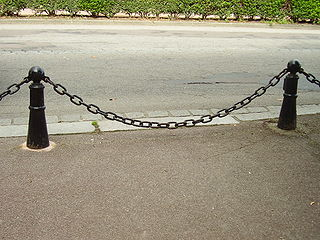
\includegraphics[scale=0.5]{figuras/catenaria.png}
		\caption{Kette Kettenkurve Catenary, Kamel15}
	\end{figure}
	
\end{frame}


\begin{frame}[label=conicas]{Por que o gráfico de uma função do $2^\circ$ é uma parábola?}
\begin{block}{Função do $2^\circ$ grau}
	\[f(x)=ax^2+bx+c, \ a\neq 0.\]
	\[y=ax^2+bx+c\]
\end{block}

\begin{exe}
\begin{enumerate}
\item Esboce a parábola $y=2x^2$, determine seu foco e a equação da reta 
diretriz
\item Use o item anterior para esboçar o gráfico de  $y=2x^2-12x+17$.
\end{enumerate}
\end{exe}

%Em particular, se $b=c=0$ e $a=1/4p$ temos que 
%\[y=\frac{1}{4p}x^2\Rightarrow x^2=4py.\]
\end{frame}





\begin{frame}[label=conicas]{Parábola com foco no eixo $OY$}
	\begin{minipage}{0.5\textwidth}
\begin{center}
	%		%	\pgfmathsetmacro{\a}{1}
	%		\pgfmathsetmacro{\b}{2}	
	\begin{tikzpicture}	
	\def\p{1}	
	\onslide<1->{\draw[scale=1,domain=-3:3,smooth,variable=\t,red,thick]
		plot ({\t},{\t*\t/(4*\p)});}
	\onslide<1->{\draw[fill,blue] (0,\p) circle (1.5pt);}
	%		\node[above right,blue] at (0,\p) {$F$};
	\draw[thick,->] (-3,0) -- (3,0) node[below] {$x$};
	\onslide<1->{\draw[dashed] (-3,-\p) -- (3,-\p) node[below right] {$\ell$};}
	\onslide<1->{\draw[thick,->] (0,-1.5) -- (0,3) node[left] {$y$}; }
	\onslide<1->{\draw[fill,red] (0,0) circle (1.5pt);
		\node[below right,red] at (0,0) {$O$};}
	\node[below left] at (0,-\p) {$-p$};
	\node[ left] at (0,\p) {$p$};
		\node[red] at (0,-3) {$x^2=4py$};
	\end{tikzpicture}
\end{center}
	\end{minipage}
	\begin{minipage}{0.3\textwidth}
	\begin{center}
		%		%	\pgfmathsetmacro{\a}{1}
		%		\pgfmathsetmacro{\b}{2}	
		\begin{tikzpicture}	
		\def\p{1}	
		\onslide<1->{\draw[scale=1,domain=-3:3,smooth,variable=\t,red,thick]
			plot ({\t},{-\t*\t/(4*\p)});}
		\onslide<1->{\draw[fill,blue] (0,-\p) circle (1.5pt);}
		%		\node[above right,blue] at (0,\p) {$F$};
		\draw[thick,->] (-3,0) -- (3,0) node[below] {$x$};
		\onslide<1->{\draw[dashed] (-3,\p) -- (3,\p) node[below right] {$\ell$};}
		\onslide<1->{\draw[thick,->] (0,-3) -- (0,1.5) node[left] {$y$}; }
		\onslide<1->{\draw[fill,red] (0,0) circle (1.5pt);
			\node[below right,red] at (0,0) {$O$};}
		\node[below left] at (0,\p) {$p$};
		\node[ left] at (0,-\p) {$-p$};
			\node[red] at (0,-4) {$x^2=-4py$};
		\end{tikzpicture}
	\end{center}
\end{minipage}
\end{frame}


\begin{frame}[label=conicas]{Parábola com foco no eixo $OX$}

\begin{minipage}{0.4\textwidth}
	\begin{center}
		%		%	\pgfmathsetmacro{\a}{1}
		%		\pgfmathsetmacro{\b}{2}	
		\begin{tikzpicture}	
		\def\p{1}	
		\onslide<1->{\draw[scale=1,domain=-2.5:2.5,smooth,variable=\t,red,thick]
			plot ({-\t*\t/(4*\p)},{\t});}
		\onslide<1->{\draw[fill,blue] (-\p,0) circle (1.5pt);}
		%		\node[above right,blue] at (0,\p) {$F$};
		\draw[thick,->] (-2.5,0) -- (2,0) node[below] {$x$};
		\onslide<1->{\draw[dashed] (\p,-2.5) -- (\p,2.5) node[below right] {$\ell$};}
		\onslide<1->{\draw[thick,->] (0,-2.5) -- (0,2.5) node[left] {$y$}; }
		\onslide<1->{\draw[fill,red] (0,0) circle (1.5pt);
			\node[below right,red] at (0,0) {$O$};}
		\node[below right] at (\p,0) {$p$};
		\node[ below] at (-\p,0) {$-p$};
		\node[red] at (0,-3) {$y^2=-4px$};
		\end{tikzpicture}
	\end{center}
\end{minipage}
\begin{minipage}{0.3\textwidth}
	\begin{center}
		%		%	\pgfmathsetmacro{\a}{1}
		%		\pgfmathsetmacro{\b}{2}	
		\begin{tikzpicture}	
		\def\p{1}	
		\onslide<1->{\draw[scale=1,domain=-2.5:2.5,smooth,variable=\t,red,thick]
			plot ({\t*\t/(4*\p)},{\t});}
		\onslide<1->{\draw[fill,blue] (\p,0) circle (1.5pt);}
		%		\node[above right,blue] at (0,\p) {$F$};
		\draw[thick,->] (-2.5,0) -- (2,0) node[below] {$x$};
		\onslide<1->{\draw[dashed] (-\p,-2.5) -- (-\p,2.5) node[below right] {$\ell$};}
		\onslide<1->{\draw[thick,->] (0,-2.5) -- (0,2.5) node[left] {$y$}; }
		\onslide<1->{\draw[fill,red] (0,0) circle (1.5pt);
			\node[below right,red] at (0,0) {$O$};}
		\node[below right] at (\p,0) {$p$};
		\node[ below] at (-\p,0) {$-p$};
		\node[red] at (0,-3) {$y^2=4px$};
		\end{tikzpicture}
	\end{center}
\end{minipage}
\end{frame}


\begin{frame}[label=conicas]
\begin{exe}
	\begin{enumerate}
		\item Determine o foco  e a equação da reta diretriz das parábolas abaixo e faça um esboço:
		\begin{enumerate}[a]
			\item $y=10x^2$
			\item $y^2=5x$
		\end{enumerate}
		
		\item Obtenha a equação da parábola de vértice em $(0,0)$ e foco em $(-8,0)$.
	\end{enumerate}
\end{exe}


\end{frame}


\begin{frame}[label=conicas]
	\begin{casa}
		
		\begin{enumerate}
			\item Determine o foco, uma equação da diretriz e faça um esboço da parábola
			\[y^2=4x\]
			
			\item Obtenha a equação da parábola de vértice em $(0,0)$ cuja diretriz tem equação $y=2$ e faça um esboço.
		\end{enumerate}
			
	\end{casa}
\end{frame}







\section{Cônicas}

\subsection*{Completamento de Quadrados}


\begin{frame}[label=comp]
	\frametitle{Completamento de Quadrados}
	%\begin{scriptsize}
	
\begin{block}{Produto Notáveis}
	\[(x+k)^2=x^2+2k\cdot x+k^2\]
	\[(x-k)^2=x^2-2k\cdot x+k^2\]
\end{block}	

\begin{exe}
	Resolva as seguintes equações sem usar a fórmula de Bhaskara
	\begin{multicols}{2}
		\begin{enumerate}
			\item $x^2-x=0$
			\item $4x^2-1=0$
			\item $x^2-2x=8$
			\item $x^2-8x=9$
		\end{enumerate}
	\end{multicols}
	\medskip
\end{exe}

\end{frame}


\begin{frame}[label=comp]
	\begin{exe}
Complete os quadrados:
\begin{enumerate}
	\item $x^2+7x$
	\item $-2x^2+8x$
\end{enumerate}
	\end{exe}

\begin{block}{Fórmula de Bhaskara}
	Sejam  $a,b$ e $c\in\R$ com $a\neq 0$. Então as soluções da equação $ax^2+bx+c=0$ são dadas por
	\[ x=\frac{-b\pm \sqrt{b^2-4ac}}{2a}\]
\end{block}
\end{frame}

\begin{frame}[label=comp]
	
\begin{casa}
	Complete os quadrados:
\begin{enumerate}
	\item $x^2-4x$
	\item $-x^2+2x$
	\item $3x^2-9x$
\end{enumerate}
\end{casa}

\end{frame}


\subsection*{Cônicas}
\begin{frame}[label=conicas]{Cônicas}

 Uma \dt{cônica}, é uma curva obtida cortando-se um
cone circular reto por um plano. As cônicas mais importantes são
as \dt{elipses, as hipérboles e as parábolas}, que ocorrem quando o plano 
cortante não passa pelo vértice do cone.

\begin{center}
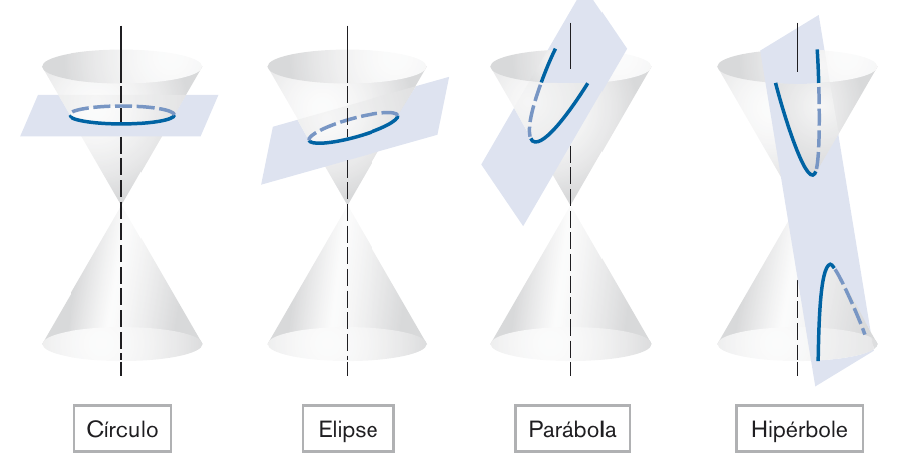
\includegraphics[scale=.4]{figuras/conicas.png}
\end{center}
%
%Os círculos são casos especiais de elipses, que resultam quando o
%plano cortante é perpendicular ao eixo de simetria do cone. Se o plano 
%cortante passa pelo vértice, então a interseção resultante é denominada uma 
%cônica degenerada, cujas possibilidades são um ponto, um par de retas que 
%se cortam ou uma única reta.
\end{frame}


\begin{frame}[label=conicas]

Em um plano cartesiano, uma equação da forma
\begin{equation*}
{\color{blue}a}{x^2}+{\color{blue}b}{y^2}
+{\color{blue}c}{xy}+{\color{blue}d}{x}
+{\color{blue}e}{y}+{\color{blue}f}=0
\end{equation*}
com \dt{$a,b$} e \dt{$c$} não todos nulos, representam uma cônica, onde também 
estão incluídos os casos das chamadas \dt{cônicas degeneradas}, cujas 
possibilidade são: \dt{um ponto}, \dt{um par de retas}, \dt{uma única 
reta} ou \dt{o conjunto vazio}.

\begin{exe}
São exemplos de cônicas que já conhecemos:
\begin{enumerate}
\item $x^2+2x-y=0$ é uma parábola.
\item $x^2+y^2=1$ é um círculo.
\item $x^2+y^2+1=0$ é o conjunto vazio.
\end{enumerate}
Qual cônica é essa
\[x^2+y^2+4x+3=0?\]
\end{exe}

\end{frame}

\subsection*{Cônicas na forma Reduzida}
\begin{frame}[label=conicas]{Cônicas na forma reduzida}
Para cada cônica, podemos escolher um sistema de eixos cartesianos de modo que a equação que a represente assuma a forma mais simples possível, chamada de \dt{equação reduzida (ou canônica)}.

\begin{itemize}
\item Elipse: $\dps\frac{x^2}{a^2}+\frac{y^2}{b^2}=1$;

\item Hipérbole: $\dps\frac{x^2}{a^2}-\frac{y^2}{b^2}=1$ ou $\dps\frac{y^2}{b^2}-\frac{x^2}{a^2}=1$;

\item Parábola: $y=ax^2$ ou $x=ay^2$.
\end{itemize}
\end{frame}


\subsection*{Elipse}
\begin{frame}[label=conicas]{Elipse}
\begin{center}
\textcolor{red}{\fbox{$\displaystyle\frac{x^2}{a^2}+\frac{y^2}{b^2}=1$}}
\end{center}
\begin{minipage}{0.4\textwidth}
	\begin{tikzpicture}[scale=0.8, every node/.style={scale=0.7}]
\node at (0,2.5) { };
	\draw[->] (-2.5,0) -- (2.5,0);
	\draw[->] (0,-1.5) -- (0,1.5);
	\node[below right] at (2.5,0) {$x$};
	\node[above left] at (0,1.5) {$y$};		
	\draw[thick,red] (0,0) ellipse (2cm and 1cm);
	\draw[fill,red] (2,0) circle (1.5pt);   	
	\draw[fill,red] (-2,0) circle (1.5pt);
	\draw[fill,red] (0,1) circle (1.5pt);   	
	\draw[fill,red] (0,-1) circle (1.5pt);
	\node[below right] at (2,0) {$a$};
	\node[below left] at (-2,0) {$-a$};
	\node[left] at (0,1.2) {$b$};
	\node[left] at (0,-1.2) {$-b$};
	\node[blue] at (0,-3) {$\displaystyle a>b$};
	\end{tikzpicture}
\end{minipage}
\begin{minipage}{0.25\textwidth}
	\begin{tikzpicture}[scale=0.7, every node/.style={scale=0.7}]
	\draw[->] (0,-2.5) -- (0,2.5);
	\draw[->] (-1.5,0) -- (1.5,0);
	\node[below right] at (1.5,0) {$x$};
	\node[above left] at (0,2.5) {$y$};		
	\draw[thick,red] (0,0) ellipse (1cm and 2cm);
%	\draw[fill,blue] (0,1.3) circle (1.5pt);
%	\draw[fill,blue] (0,-1.3) circle (1.5pt);   
%	\node[left] at (0,1.3) {$c$};
%	\node[left] at (0,-1.3) {$-c$};
	\draw[fill,red] (0,2) circle (1.5pt);   	
	\draw[fill,red] (0,-2) circle (1.5pt);
	\draw[fill,red] (1,0) circle (1.5pt);   	
	\draw[fill,red] (-1,0) circle (1.5pt);
	\node[left] at (0,2.2) {$b$};
	\node[left] at (0,-2.2) {$-b$};
	\node[below] at (1.2,0) {$a$};
	\node[below] at (-1.3,0) {$-a$};
	\node[blue] at (0,-3.5) {$\displaystyle b>a$};
	\end{tikzpicture}
\end{minipage}
\begin{minipage}{0.2\textwidth}
	\begin{tikzpicture}[scale=0.7, every node/.style={scale=0.7}]
	\draw[->] (-2.5,0) -- (2.5,0);
	\draw[->] (0,-2.5) -- (0,2.5);
	\node[below right] at (2.5,0) {$x$};
	\node[above left] at (0,2.5) {$y$};		
	\draw[thick,red] (0,0) ellipse (2cm and 2cm);
	\draw[fill,red] (2,0) circle (1.5pt);   	
	\draw[fill,red] (-2,0) circle (1.5pt);
	\draw[fill,red] (0,2) circle (1.5pt);   	
	\draw[fill,red] (0,-2) circle (1.5pt);
	\node[below right] at (2,0) {$a$};
	\node[below left] at (-2,0) {$-a$};
	\node[left] at (0,2.2) {$a$};
	\node[left] at (0,-2.2) {$-a$};
	\node[blue] at (0,-3.5) {$\displaystyle a=b$};
	\end{tikzpicture}
\end{minipage}

\end{frame}

\subsection*{Hipérbole}
\begin{frame}[label=conicas]{Hipérbole}
%\begin{center}
%\textcolor{red}{\fbox{$\displaystyle\frac{x^2}{a^2}-\frac{y^2}{b^2}=1$}}
%\end{center}
 \ \ \ \ \ \begin{minipage}{0.6\textwidth}
\qquad\quad
{\color{red}\fbox{$\displaystyle\frac{x^2}{a^2}-\frac{y^2}{b^2}=1$}}
\bigskip

\begin{tikzpicture}[scale=0.7, every node/.style={scale=0.7}]
\def\a{1.5}	
\def\b{1}			

\coordinate (AB) at (\a,\b);
\coordinate (ABm) at (-\a,-\b);
\coordinate (mAB) at (-\a,\b);
\coordinate (AmB) at (\a,-\b);

%\node[red] at (0,4) {$\displaystyle\frac{x^2}{a^2}-\frac{y^2}{b^2}=1$};
\draw[domain=-1.5:1.5,smooth,variable=\t,red,thick]
plot ({\a*cosh(\t )},{\b*sinh(\t)});
\draw[domain=-1.5:1.5,smooth,variable=\t,red,thick]
plot ({-\a*cosh(\t )},{\b*sinh(\t)});

\draw[->] (-3.5,0) -- (3.5,0);
\draw[->] (0,-2.) -- (0,2);
\node[below right] at (3.5,0) {$x$};
\node[above left] at (0,2) {$y$};

\draw [shorten >= -2.cm, shorten <=-2.cm,dashed] (AB)--(ABm);
\draw [shorten >= -2.cm, shorten <=-2.cm,dashed] (mAB)--(AmB);
\draw[dashed] (AB) -- (AmB) -- (ABm) -- (mAB) -- (AB);

\draw[fill,red] (\a,0) node[below left] {$a$} circle (1.5pt);
\draw[fill,red] (-\a,0) node[below right] {$-a$} circle (1.5pt);

	\draw[fill] (0,\b) node[above left] {$b$} circle (1.5pt);
\draw[fill] (0,-\b) node[below left] {$-b$} circle (1.5pt);
\end{tikzpicture}
\end{minipage}
\begin{minipage}{0.3\textwidth}

{\color{red}\fbox{$\displaystyle\frac{y^2}{b^2}-\frac{x^2}{a^2}=1$}}
\bigskip

\begin{tikzpicture}[scale=0.7, every node/.style={scale=0.7}]	
\def\a{1.5}	
\def\b{1}		

\coordinate (AB) at (\b,\a);
\coordinate (ABm) at (-\b,-\a);
\coordinate (mAB) at (-\b,\a);
\coordinate (AmB) at (\b,-\a);		

\draw[domain=-1.5:1.5,smooth,variable=\t,red,thick]
plot ({\b*sinh(\t)},{\a*cosh(\t )});
\draw[domain=-1.5:1.5,smooth,variable=\t,red,thick]
plot ({\b*sinh(\t)},{-\a*cosh(\t )});

\draw[->] (0,-3.5) -- (0,3.5);
\draw[->] (-2,0) -- (2,0);
\node[below right] at (2,0) {$x$};
\node[above left] at (0,3.5) {$y$};

\draw [shorten >= -2.cm, shorten <=-2.cm,dashed] (AB)--(ABm);
\draw [shorten >= -2.cm, shorten <=-2.cm,dashed] (mAB)--(AmB);
\draw[dashed] (AB) -- (AmB) -- (ABm) -- (mAB) -- (AB);

\draw[fill,red] (0,\a) node[below left] {$b$} circle (1.5pt);
\draw[fill,red] (0,-\a) node[above left] {$-b$} circle (1.5pt);

\draw[fill] (\b,0) node[below] {$a$} circle (1.5pt);
\draw[fill] (-\b,0) node[below] {$-a$} circle (1.5pt);

\end{tikzpicture}
\end{minipage}
\end{frame}


\subsection*{Parábola}
\begin{frame}[label=conicas]{Parábola}

\qquad\begin{minipage}{0.5\textwidth}
\quad
{\footnotesize {\color{red}\fbox{$\displaystyle y=ax^2, \ a>0$}}}


\begin{tikzpicture}[scale=0.5, every node/.style={scale=0.6}]	
	\def\p{1}	
\onslide<1->{\draw[scale=1,domain=-3:3,smooth,variable=\t,red,thick]
	plot ({\t},{\t*\t/(4*\p)});}
\draw[thick,->] (-3,0) -- (3,0) node[below] {$x$};
\draw[thick,->] (0,-1.5) -- (0,3) node[left] {$y$}; 
\draw[fill,red] (0,0) circle (1.5pt);
\node[below right,red] at (0,0) {$O$};

\end{tikzpicture}
\end{minipage}
\begin{minipage}{0.3\textwidth}
\quad
{\footnotesize {\color{red}\fbox{$\displaystyle y=-ax^2, \ a>0$}}}
\bigskip

\begin{tikzpicture}[scale=0.5, every node/.style={scale=0.6}]
\def\p{1}	
\draw[scale=1,domain=-3:3,smooth,variable=\t,red,thick]
	plot ({\t},{-\t*\t/(4*\p)});

\draw[thick,->] (-3,0) -- (3,0) node[below] {$x$};
\draw[thick,->] (0,-2.5) -- (0,1.5) node[left] {$y$}; 
\draw[fill,red] (0,0) circle (1.5pt);
\node[below right,red] at (0,0) {$O$};

\end{tikzpicture}
\end{minipage}
\bigskip
\bigskip

\qquad\begin{minipage}{0.5\textwidth}
\quad
{\footnotesize {\color{red}\fbox{$\displaystyle x=ay^2, \ a>0$}}}


\begin{tikzpicture}[scale=0.5, every node/.style={scale=0.7}]
\def\p{1}	
\draw[scale=1,domain=-2.5:2.5,smooth,variable=\t,red,thick]
	plot ({-\t*\t/(4*\p)},{\t});
\draw[thick,->] (-2.5,0) -- (2,0) node[below] {$x$};
\draw[thick,->] (0,-2.5) -- (0,2.5) node[left] {$y$}; 
\draw[fill,red] (0,0) circle (1.5pt);
\node[below right,red] at (0,0) {$O$};

\end{tikzpicture}
\end{minipage}
\begin{minipage}{0.3\textwidth}
\qquad\quad
{\footnotesize {\color{red}\fbox{$\displaystyle x=-ay^2, \ a>0$}}}


\begin{tikzpicture}[scale=0.5, every node/.style={scale=0.7}]	
\def\p{1}	
\draw[scale=1,domain=-2.5:2.5,smooth,variable=\t,red,thick]
	plot ({\t*\t/(4*\p)},{\t});
\draw[thick,->] (-2.5,0) -- (2,0) node[below] {$x$};
\draw[thick,->] (0,-2.5) -- (0,2.5) node[left] {$y$}; 
\draw[fill,red] (0,0) circle (1.5pt);
\node[below right,red] at (0,0) {$O$};

\end{tikzpicture}
\end{minipage}

\end{frame}

\begin{frame}[label=conicas]
\begin{exe}
Identifique as cônicas abaixo e faça um esboço.
\begin{enumerate}
\item $4x^2+9y^2=36$
\item $5x^2-2y^2=15$
\item $4x^2-9y=0$
\item $y^2=5x$
\end{enumerate}
\end{exe}

\end{frame}

\subsection*{Curvas que não são parábolas}
\begin{frame}[label=conicas]{Curvas que não são parábolas}
	\begin{enumerate}
		\item $y=x^4$
		\item $y=\cosh x=\frac{e^x+e^{-x}}{2}$  ( catenária ) 
	\end{enumerate}
	
	
	Quando um cabo flexível pesado é suspenso entre dois pontos  na mesma altura, vemos a formação de uma curva conhecida como \dest{catenária}, do latim \textit{catena} que significa corrente. 
	\begin{figure}
		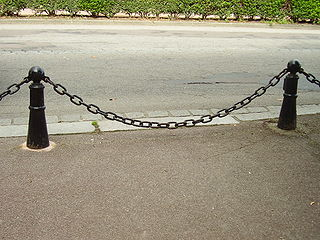
\includegraphics[scale=0.5]{figuras/catenaria.png}
		\caption{Kette Kettenkurve Catenary, Kamel15}
	\end{figure}
	
\end{frame}


\begin{frame}[label=conicas]{Por que o gráfico de uma função do $2^\circ$ é uma parábola?}
\begin{block}{Função do $2^\circ$ grau}
	\[f(x)=ax^2+bx+c, \ a\neq 0.\]
	\[y=ax^2+bx+c\]
\end{block}

\begin{exe}
Façao o completamento de quadrado e esboçe o gráfico de  
\[y=2x^2-12x+17.\]
\end{exe}

%Em particular, se $b=c=0$ e $a=1/4p$ temos que 
%\[y=\frac{1}{4p}x^2\Rightarrow x^2=4py.\]
\end{frame}


\subsection*{Cônicas Transladadas}
\begin{frame}[label=conicas]{Cônicas Transladadas}

\begin{center}
{\color{blue} Mudança de coordenadas }
\end{center}
\begin{equation*}
	\begin{cases}
		\textcolor{blue}{x'}=x-x_0\\
		\textcolor{blue}{y'}=y-y_0.
	\end{cases}
\end{equation*}

\begin{tikzpicture}[scale=0.7]

\usetikzlibrary{decorations.pathreplacing} 
\tikzset{>=latex}
%\draw[help lines, color=gray!30, dashed] (0,0) grid (6,6);

%sistema de eixos e ponto P
\draw[->,thick] (-.5,0)--(6,0) node[right]{$x$};
\draw[->,thick] (0,-.5)--(0,6) node[above]{$y$};
\node at (0,0) {\textbullet};
\node[below left] at (0,0) {$O$};
\node at (4,4) {\textbullet};
\node[above right] at (4,4) {$P$};
\draw[dashed] (4,0) -- (4,4) -- (0,4);
\node[below ] at (4,0) {$x$};
\node[left] at (0,4) {$y$};

%ponto de translação
\uncover<2->{
\node[blue] at (1.5,2) {\textbullet};
\node[below left,blue] at (1.5,2) {$O'$};
\node[below left] at (1.5,0) {$x_0$};
\node[below left] at (0,2) {$y_0$};
\draw[dashed] (1.5,0)--(1.5,2)--(0,2);
}


\uncover<3->{
\draw[->,thick,blue] (-.5,2)--(6,2) node[right]{$x'$};
\draw[->,thick,blue] (1.5,-.5)--(1.5,6) node[above]{$y'$};
}

\uncover<4->{
\node[below left,blue] at (4,2) {$x'$};
\node[below left,blue] at (1.5,4) {$y'$};

\draw[thick,decoration={brace,mirror,raise=0.5cm},decorate,blue] (1.5,0) --   (4,0)
node[pos=0.5,anchor=north,yshift=-0.55cm,blue] {$x-x_0$};
\draw[thick,decoration={brace,raise=0.5cm},decorate,blue] (0,2) --   (0,4)
node[pos=0.5,anchor=east,xshift=-0.55cm,blue] {$y-y_0$};}

\end{tikzpicture}


\end{frame}


\begin{frame}[label=conicas]

As equações de cônicas que não apresentam termos mistos da forma $xy$ 
podem  ser colocadas na forma reduzida através de uma translação de 
eixos.

\begin{exe}
Identifique e faça o esboço das cônicas a seguir:

\begin{enumerate}
\item $x^2+2y^2-6x+8y+9=0$.
\item $4x^2-16y^2-24x-24y+33=0$.
\end{enumerate}
\end{exe}

\end{frame}

\subsection*{Cônicas Rotacionadas}

\begin{frame}[label=conicas]{Cônicas Rotacionadas}
Os termos mistos da forma $xy$ de uma equação de cônica podem ser 
eliminados através de um processo de diagonalização, que equivale a uma 
rotação dos eixos.
\medskip

Uma expressão da forma
\[{\color{blue}a}x^2+{\color{blue}b}y^2+{\color{blue}c}xy\]
é chamada de \dt{forma quadrática} em $x$ e $y$ e pode ser representada 
usando matrizes da seguinte forma:
\[{\color{blue}a}x^2+{\color{blue}b}y^2+{\color{blue}c}xy=
\begin{bmatrix}
x & y
\end{bmatrix}
{\color{blue}\begin{bmatrix}
a & c/2\\ c/2 & b
\end{bmatrix}}
\begin{bmatrix}
x \\ y
\end{bmatrix}= X^t {\color{blue}A} X.
\]

\end{frame}


\begin{frame}[label=conicas]{Teorema dos Eixos Principais}
Como ${\color{blue}A}$ é uma matriz simétrica, pelo Teorema Espectral, 
existe uma matriz ortogonal que diagonaliza ${\color{blue}A}$, isto é, 
\[Q^t {\color{blue}A} Q={\color{red}D},\]
onde ${\color{red}D}$ é uma matriz diagonal formada por autovalores de 
${\color{blue}A}$.
Fazendo a \dt{mudança de variáveis} 
\[X=Q\bar{X}\ \text{ ou, equivalentemente, }\  \bar{X}=Q^tX,\]
temos
\begin{equation*}
X^t {\color{blue}A} X
=(Q\bar{X})^t {\color{blue}A}(Q\bar{X})
=\bar{X}^t(Q^t {\color{blue}A}Q) \bar{X}
=\bar{X}^t{\color{red}D}\bar{X}
\end{equation*}



\end{frame}

\begin{frame}[label=conicas]{Teorema dos Eixos Principais}
Assim, se ${\color{red}\lambda_1,\lambda_2}$ são os autovalores de ${\color{blue}A}$ e 
\[\bar{X}=
\begin{bmatrix}
\bar{x} \\ \bar{y},
\end{bmatrix}\]
então
\begin{align*}
{\color{blue}a}x^2+{\color{blue}b}y^2+{\color{blue}c}xy& =X^t {\color{blue}A} X\\
& =\bar{X}^t{\color{red}D}\bar{X}\\
& = {\color{red}\lambda_1}\bar{x}^2+{\color{red}\lambda_2}\bar{y}^2,
\end{align*}
uma forma quadrática sem termos mistos.

\end{frame}


\begin{frame}[label=conicas]
\begin{exe}
Identifique e faça um esboça das seguintes cônicas:
\begin{enumerate}
\item $5x^2+4xy+2y^2=6$.
\item $2x^2-4xy-y^2+8=0.$
\item $x^2+4\sqrt{2}xy-y^2+2\sqrt{6}x+2\sqrt{3}y=0$
\end{enumerate}
\end{exe}
\end{frame}


\begin{frame}[label=conicas]
\begin{casa}
Identifique e faça um esboço das seguintes cônicas

\begin{enumerate}
\item  $5x^2-4xy+8y^2-36=0$
\item $11 x^{2} + 24 x y + 4 x + 4 y^{2} + 3 y + \frac{15}{4} = 0$
\end{enumerate}
\end{casa}
\end{frame}

\begin{frame}[label=conicas]



\end{frame}






\end{document}
